\documentclass[12pt,a4paper]{article}

% Inclusão de configurações, pacotes e comandos visuais
% ==============================================================================
% PACOTES BÁSICOS E TIPOGRAFIA
% ==============================================================================
\usepackage[utf8]{inputenc}
\usepackage[T1]{fontenc}
% Tradução e termos em Português
\renewcommand{\contentsname}{Sumário}
\renewcommand{\figurename}{Figura}
\renewcommand{\tablename}{Tabela}
\renewcommand{\refname}{Referências Bibliográficas}
\usepackage{lmodern}

% ==============================================================================
% MATEMÁTICA E SÍMBOLOS
% ==============================================================================
\usepackage{amsmath}
\usepackage{amssymb}
\usepackage{amsfonts}

% ==============================================================================
% LAYOUT, TABELAS E FORMATAÇÃO
% ==============================================================================
\usepackage{geometry}
\geometry{left=3cm,right=2cm,top=3cm,bottom=2cm}
\usepackage{setspace}
\usepackage{booktabs}
\usepackage{tabularx}
\usepackage{xltabular}
\usepackage{multirow}
\usepackage{enumitem}
\usepackage{microtype}
\usepackage{float}

% ==============================================================================
% CORES E ELEMENTOS GRÁFICOS
% ==============================================================================
\usepackage{xcolor}
\definecolor{vitalisblue}{RGB}{24, 76, 120}
\definecolor{vitalisdark}{RGB}{18, 52, 86}
\definecolor{vitalislight}{RGB}{230, 240, 250}
\definecolor{vitalisred}{RGB}{180, 40, 40}
\definecolor{vitalisgreen}{RGB}{34, 139, 34}
\definecolor{vitalisgray}{RGB}{100, 110, 120}
\definecolor{codebg}{RGB}{245, 247, 250}

\usepackage{graphicx}

% ==============================================================================
% TIKZ E DIAGRAMAS (BPMN, UML, CLASSES, CASOS DE USO)
% ==============================================================================
\usepackage{tikz}
\usetikzlibrary{
    shapes.geometric,
    shapes.misc,
    shapes.multipart,
    arrows.meta,
    positioning,
    calc,
    fit,
    backgrounds,
    decorations.pathreplacing,
    matrix,
    shadows
}

% ==============================================================================
% CRONOGRAMA E MARCOS (PGFGANTT)
% ==============================================================================
\usepackage{pgfgantt}

% ==============================================================================
% CÓDIGO-FONTE E LISTINGS
% ==============================================================================
\usepackage{listings}
\lstset{
    backgroundcolor=\color{codebg},
    basicstyle=\ttfamily\footnotesize,
    breaklines=true,
    captionpos=b,
    frame=single,
    rulecolor=\color{vitalisgray!40},
    numbers=left,
    numberstyle=\tiny\color{vitalisgray},
    keywordstyle=\color{vitalisblue}\bfseries,
    commentstyle=\color{vitalisgreen}\itshape,
    stringstyle=\color{vitalisred}
}

% ==============================================================================
% HIPERLINKS E CITAÇÕES
% ==============================================================================
\usepackage{hyperref}
\hypersetup{
    colorlinks=true,
    linkcolor=vitalisblue,
    citecolor=vitalisdark,
    urlcolor=vitalisblue,
    pdfstartview={FitH}
}

% ==============================================================================
% DEFINIÇÕES DE ESTILOS TIKZ PARA BPMN E UML NATIVOS NO OVERLEAF
% ==============================================================================

% --- BPMN Styles ---
\tikzstyle{bpmnStart} = [circle, draw=vitalisgreen!80!black, fill=vitalisgreen!15, line width=1.5pt, minimum size=8mm]
\tikzstyle{bpmnEnd} = [circle, draw=vitalisred!80!black, fill=vitalisred!15, line width=2.5pt, minimum size=8mm]
\tikzstyle{bpmnTask} = [rectangle, rounded corners=3pt, draw=vitalisblue!90, fill=vitalisblue!8, line width=1pt, minimum width=2.5cm, minimum height=1.1cm, text centered, text width=2.3cm, font=\scriptsize\sffamily]
\tikzstyle{bpmnAiTask} = [rectangle, rounded corners=3pt, draw=purple!80!black, fill=purple!8, line width=1.2pt, minimum width=2.5cm, minimum height=1.1cm, text centered, text width=2.3cm, font=\scriptsize\sffamily]
\tikzstyle{bpmnGateway} = [diamond, draw=orange!90!black, fill=orange!15, line width=1.2pt, minimum size=9mm, text centered, font=\scriptsize\sffamily]
\tikzstyle{bpmnArrow} = [-{Latex[length=2.5mm]}, draw=vitalisdark, line width=0.9pt]
\tikzstyle{bpmnDashArrow} = [-{Latex[length=2.5mm]}, dashed, draw=vitalisgray, line width=0.8pt]

% --- UML Class Diagram Styles ---
\tikzstyle{umlClass} = [rectangle, draw=vitalisdark, fill=vitalislight!40, line width=1pt, text width=3.8cm, font=\scriptsize\sffamily]
\tikzstyle{umlAiClass} = [rectangle, draw=purple!80!black, fill=purple!5, line width=1.2pt, text width=4.0cm, font=\scriptsize\sffamily]

% --- UML Use Case Styles ---
\tikzstyle{umlActor} = [circle, draw=vitalisdark, fill=vitalisdark!20, minimum size=5mm, line width=1pt]
\tikzstyle{umlUseCase} = [ellipse, draw=vitalisblue, fill=vitalisblue!8, line width=1pt, text centered, minimum width=3.2cm, minimum height=1.1cm, text width=3.0cm, font=\scriptsize\sffamily]
\tikzstyle{umlInclude} = [-{Latex[length=2mm]}, dashed, draw=vitalisgray, font=\tiny\itshape]
\tikzstyle{umlExtend} = [-{Latex[length=2mm]}, dashed, draw=vitalisred!80, font=\tiny\itshape]

% --- Box de Destaque / Callout ---
\newcommand{\destaqueVitalis}[2]{%
    \begin{center}
    \fcolorbox{vitalisblue!60}{vitalislight!50}{%
        \parbox{0.95\textwidth}{%
            \vspace{0.3em}
            \textbf{\color{vitalisdark}#1}\par
            \vspace{0.2em}
            \small #2
            \vspace{0.3em}
        }%
    }
    \end{center}
}


\begin{document}

% ==============================================================================
% CAPA INSTITUCIONAL UCSAL
% ==============================================================================
\begin{titlepage}
    \centering
    \vspace*{1.0cm}
    {\large \textbf{UNIVERSIDADE CATÓLICA DO SALVADOR -- UCSAL}}\\[0.3cm]
    {\large \textbf{ESCOLA DE TECNOLOGIAS}}\\[0.3cm]
    {\large \textbf{CURSO DE ENGENHARIA DE SOFTWARE}}\\[0.3cm]
    {\large \textbf{DISCIPLINA: TÓPICOS AVANÇADOS DE PROGRAMAÇÃO}}\\[0.3cm]
    {\large \textbf{PROFESSOR: ELTON FIGUEIREDO DA SILVA}}\\[3.5cm]

    {\LARGE \textbf{\color{vitalisdark}SISTEMA DE GESTÃO HOSPITALAR INTELIGENTE}}\\[0.4cm]
    {\huge \textbf{\color{vitalisblue}VITALIS (VERSÃO 2.0)}}\\[0.8cm]
    {\large \textbf{DOCUMENTAÇÃO DE ENGENHARIA DE SOFTWARE, ARQUITETURA E MODELAGEM DE PROCESSOS COM INTELIGÊNCIA ARTIFICIAL CLÍNICA}}\\[3.5cm]

    \begin{flushright}
        \begin{minipage}{0.55\textwidth}
            \small
            \textbf{Acadêmico:} Davi dos Santos Ribeiro\\
            \textbf{Matrícula / E-mail:} davi.ribeiro@ucsal.edu.br\\
            \textbf{Projeto:} Documentação Técnica Integral (Requisitos, BPMN, Classes, Casos de Uso, Cronograma e Módulo de IA)
        \end{minipage}
    \end{flushright}

    \vfill
    {\large Salvador -- BA\\ Outubro de 2026}
\end{titlepage}

% ==============================================================================
% ELEMENTOS PRÉ-TEXTUAIS (SUMÁRIO, LISTAS)
% ==============================================================================
\pagenumbering{roman}
\tableofcontents
\newpage

\listoffigures
\vspace{1.5cm}
\listoftables
\newpage

\pagenumbering{arabic}
\setcounter{page}{1}

% ==============================================================================
% SEÇÕES DO PROJETO VITALIS v2.0
% ==============================================================================
% ==============================================================================
% SEÇÃO 1: DESCRITIVO DETALHADO DO SISTEMA VITALIS v2.0
% ==============================================================================

\section{Descritivo Detalhado do Sistema Vitalis v2.0}
\label{sec:descritivo}

O Sistema de Gestão Hospitalar Inteligente Vitalis (Versão 2.0) é uma plataforma integrada de prontuário eletrônico do paciente (PEP), regulação de leitos e suporte à decisão clínica, projetada para atender às demandas de hospitais gerais e de alta complexidade. A solução combina a gestão dos processos administrativos e assistenciais com modelos de inteligência artificial preditiva e generativa, atuando como camada consultiva para médicos, enfermeiros, farmacêuticos e gestores. Esta seção apresenta o contexto operacional da instituição hospitalar, a arquitetura de microsserviços, o ciclo assistencial completo do paciente, os módulos especializados de inteligência artificial e as salvaguardas éticas e legais do projeto.

\subsection{Contexto Operacional e Visão de Negócio}
\label{subsec:contexto_negocio}

Ambientes hospitalares terciários operam sob contínua sobrecarga cognitiva, com fluxos assistenciais simultâneos em unidades de pronto atendimento, enfermarias de internação, centros cirúrgicos e unidades de terapia intensiva (UTI). Nesses cenários, a fragmentação dos dados entre sistemas legados desconectados gera gargalos crônicos:

\begin{itemize}
    \item Retardo na identificação de pacientes em risco de deterioração clínica rápida ou sepse nas primeiras horas de triagem;
    \item Erros decorrentes da transcrição manual repetitiva de sinais vitais, queixas clínicas e planos terapêuticos;
    \item Ociosidade invisível de leitos em decorrência da falta de sincronismo entre a alta médica, o serviço de higienização predial e a regulação central;
    \item Glosas financeiras frequentes provocadas por inconsistências documentais entre as prescrições médicas executadas e os itens faturados nas guias da saúde suplementar.
\end{itemize}

O Vitalis v2.0 unifica esses domínios em uma plataforma digital integrada. O propósito operacional é reduzir o tempo de espera no acolhimento, maximizar a rotatividade segura dos leitos por meio da antecipação da demanda assistencial e zerar glosas administrativas decorrentes de falhas de preenchimento. A plataforma prioriza a segurança do paciente e o rigor assistencial, de modo que todo modelo preditivo ou generativo atua estritamente como suporte técnico subordinado à homologação do profissional responsável \cite{topol:2019}.

\subsection{Arquitetura em Microsserviços e Engenharia de Software}
\label{subsec:arquitetura_software}

Para garantir disponibilidade contínua, tolerância a falhas e isolamento de domínios funcionais, o Vitalis v2.0 adota uma arquitetura orientada a microsserviços fundamentada nas seguintes escolhas de engenharia:

\begin{itemize}
    \item \textbf{Camada de Serviços e APIs}: Cada microsserviço é construído sobre o framework NestJS utilizando o motor de rede Fastify, o que assegura baixa latência sob alta concorrência de conexões. O código adota TypeScript com separação em camadas inspirada na Arquitetura Limpa, isolando entidades de domínio, casos de uso e adaptadores de infraestrutura.
    \item \textbf{Orquestração de Filas e Tarefas Assíncronas}: O sistema emprega o BullMQ suportado por instâncias em memória do Redis. Essa estrutura gerencia o processamento assíncrono de tarefas com alto custo computacional, tais como chamadas a modelos de linguagem, indexação vetorial de literatura médica, geração de laudos em PDF e compilação de lotes de guias TISS. Filas prioritárias garantem que alertas de deterioração clínica sejam despachados em milissegundos, enquanto rotinas financeiras operam em baixa prioridade.
    \item \textbf{Persistência Relacional em Terceira Forma Normal (3NF)}: A persistência operacional utiliza o PostgreSQL. O esquema de dados é normalizado rigorosamente em 3NF \cite{pressman:2016}, eliminando redundâncias indesejadas e inconsistências funcionais. O modelo estrutura tabelas nucleares como \texttt{PACIENTE}, \texttt{ATENDIMENTO}, \texttt{PRONTUARIO\_LOGICO}, \texttt{EVOLUCAO}, \texttt{PRESCRICAO}, \texttt{LEITO} e \texttt{GUIA\_TISS}, utilizando índices compostos otimizados para consultas de séries temporais de sinais vitais e histórico do prontuário.
    \item \textbf{Controle de Acesso Granular (RBAC e ABAC)}: A autorização combina papéis hierárquicos com atributos de contexto, tais como registro ativo em conselhos profissionais (CRM, COREN, CRF), especialidade clínica cadastrada e vinculação formal ao episódio de cuidado ativo do paciente. Usuários administrativos não possuem permissão de acesso a notas confidenciais de saúde mental.
    \item \textbf{Comunicação em Tempo Real}: A sincronização do mapa de leitos e o disparo de alertas emergenciais utilizam WebSockets bidirecionais, atualizando imediatamente os terminais dos postos de enfermagem sem exigir recarregamento manual de página.
    \item \textbf{Gateway de IA Seguro e Anonimizador}: Todas as solicitações direcionadas a serviços de IA transitam obrigatoriamente por um gateway intermediário. Esse serviço executa inspeção de payload, remove identificadores pessoais e formata os dados clínicos antes da inferência, protegendo a privacidade dos dados.
    \item \textbf{Resiliência via Circuit Breaker}: Se um serviço externo de inferência atingir latência superior a 2,0 segundos ou apresentar falha de resposta, o sistema chaveia automaticamente para mecanismos determinísticos locais baseados em árvores de decisão e tabelas clínicas tradicionais, preservando a continuidade operacional sem interrupções.
\end{itemize}

\subsection{Ciclo Assistencial Completo do Paciente}
\label{subsec:ciclo_assistencial}

O Vitalis v2.0 gerencia todo o percurso assistencial e administrativo do paciente no hospital e assegura a rastreabilidade integral em cada etapa do fluxo.

\subsubsection{Recepção e Admissão Cadastral}
O ciclo se inicia com a identificação do paciente na recepção hospitalar. O sistema valida os dígitos verificadores do CPF junto às regras cadastrais da Receita Federal e consulta o número do Cartão Nacional de Saúde (CNS). Em casos de emergência com pacientes inconscientes ou não identificados, o sistema permite a abertura imediata de prontuário sob o protocolo provisório de "Paciente Desconhecido", exigindo regularização cadastral posterior. Para pacientes de saúde suplementar, o módulo executa a verificação eletrônica de elegibilidade da operadora de saúde e gera o token de atendimento, posicionando o paciente na fila de acolhimento.

\subsubsection{Acolhimento e Triagem Aumentada por IA}
Na sala de classificação de risco, o enfermeiro triador realiza a avaliação do paciente fundamentada no Protocolo de Manchester \cite{manchester:2014}. O sistema disponibiliza entrada via formulário estruturado e módulo de reconhecimento de voz (Speech-to-Text via Whisper), transcrevendo as queixas do paciente e convertendo a linguagem natural em descritores clínicos objetivos.

Enquanto o profissional afere os parâmetros vitais (frequência cardíaca, pressão arterial sistólica e diastólica, saturação periférica de oxigênio, frequência respiratória e escala de coma de Glasgow), o Vitalis v2.0 executa em paralelo o cálculo automatizado de dois escores clínicos de gravidade:
\begin{itemize}
    \item \textbf{qSOFA} (\textit{Quick Sequential Organ Failure Assessment}): Pontua alterações em frequência respiratória ($\ge 22\,\text{rpm}$), pressão arterial sistólica ($\le 100\,\text{mmHg}$) e estado neurológico, alertando para risco elevado de sepse em pacientes fora da UTI \cite{singer_sepsis:2016};
    \item \textbf{NEWS2} (\textit{National Early Warning Score 2}): Agrega os parâmetros fisiológicos para mensurar o grau de estresse hemodinâmico e prever risco iminente de colapso respiratório ou necessidade de leito intensivo.
\end{itemize}
Se a classificação resultar na prioridade Vermelha (Emergência), o sistema ativa avisos visuais e sonoros nos monitores da sala de emergência e transfere o paciente para o topo absoluto da fila médica.

\subsubsection{Regulação e Alocação Preditiva de Leitos}
Após a avaliação médica indicar a necessidade de internação, entra em ação o módulo de gestão de leitos. A plataforma apresenta um mapa visual com o estado de cada vaga: Livre, Reservado, Ocupado, Em Higienização, Manutenção ou Isolamento.

O motor analítico de previsão de tempo de permanência (\textit{Length of Stay}, LOS) utiliza algoritmos treinados sobre variáveis demográficas, diagnóstico principal CID-10, histórico de comorbidades e complexidade de procedimentos solicitados. O sistema estima o período médio de internação e indica a melhor acomodação disponível por ala e especialidade. O fluxo proíbe a transferência para leitos marcados como "Em Higienização" antes da validação digital pela equipe de hotelaria hospitalar.

\subsubsection{Prontuário Eletrônico (PEP) e Copiloto Farmacoterapêutico}
Durante a estada hospitalar, todas as anotações clínicas, ordens de serviço, solicitações de exames diagnósticos e prescrições médicas são concentradas no PEP. O módulo de prescrição eletrônica conta com um copiloto farmacoterapêutico baseado em arquitetura RAG (\textit{Retrieval-Augmented Generation}) \cite{lewis_rag:2020}.

Esse copiloto recupera informações em uma base vetorial que reúne bulários, guias de diluição, monografias de interações e diretrizes clínicas institucionais. Ao selecionar um medicamento, o motor faz a checagem cruzada das seguintes variáveis:
\begin{itemize}
    \item Alergias ativas e reações adversas prévias registradas no perfil do paciente;
    \item Interações farmacológicas entre os itens da prescrição atual e prescrições vigentes;
    \item Ajuste de dosagem por faixa de peso corporal e função renal calculada com base na creatinina sérica recente;
    \item Duplicidade de classes terapêuticas e incompatibilidades físico-químicas de administração pela mesma via venosa.
\end{itemize}
Caso seja detectada uma incompatibilidade moderada ou grave, o sistema exibe alertas contextualizados e exige a concordância justificada do médico para autorizar o despacho à farmácia satélite.

\subsubsection{Evoluções Clínicas e Sumário de Alta Automatizado}
Os médicos e a equipe multiprofissional registram evoluções diárias estruturadas por sistemas orgânicos (Cardiovascular, Respiratório, Neurológico, Gastrointestinal e Renal). Quando o paciente atinge estabilidade clínica e preenche os critérios para desospitalização, o médico aciona a geração automatizada do sumário de alta.

O modelo de linguagem agrega os marcos temporais da internação: motivo da admissão, diagnósticos confirmados, procedimentos cirúrgicos executados, exames laboratoriais e radiológicos com resultados anormais, fármacos administrados e resposta terapêutica. O sistema compõe uma minuta formal contendo o resumo do internamento, a receita médica de continuidade domiciliar e o plano de retorno ambulatorial. O médico analisa o texto, realiza as modificações pertinentes e assina o documento.

\subsubsection{Faturamento Hospitalar e Auditoria TISS/TUSS}
Após a assinatura da alta, o atendimento é disponibilizado ao setor de faturamento. O sistema compila automaticamente os itens consumidos (diárias de quarto, taxas de uso de sala cirúrgica, gases medicinais, exames realizados, medicamentos dispensados e honorários profissionais).

O motor de auditoria preventiva confronta esses lançamentos com a tabela de cobertura do convênio e as regras de codificação TUSS estabelecidas pela Agência Nacional de Saúde Suplementar (ANS) \cite{ans_tiss:2023}. O sistema detecta preventivamente discrepâncias como cobrança de antibióticos de uso restrito sem laudo de cultura comprobatório anexado, cobranças de taxas cirúrgicas incompatíveis com o tempo de anestesia ou ausência de autorização prévia da operadora. Isso permite a correção documental pelo faturista antes da transmissão do lote XML, reduzindo a incidência de glosas.

\subsection{Módulos Especializados de Inteligência Artificial e Suporte à Decisão}
\label{subsec:modulos_ia}

A camada de inteligência do Vitalis v2.0 é organizada em quatro pipelines de processamento focados em pontos críticos do atendimento:

\begin{itemize}
    \item \textbf{Processamento de Linguagem Natural e Reconhecimento de Voz}: Responsável por converter o áudio da anamnese em texto estruturado durante a triagem. O módulo utiliza reconhecimento fonético calibrado para terminologia médica em língua portuguesa, identificando entidades clínicas como sintomas, dosagens e tempo de evolução da queixa.
    \item \textbf{Motor Preditivo de Risco Hemodinâmico}: Calcula continuamente os escores qSOFA e NEWS2 a partir de novas entradas de sinais vitais e exames laboratoriais. O modelo opera com pesos calibrados para evitar alarmes espúrios, mantendo alta sensibilidade para detecção precoce de sepse e insuficiência respiratória aguda.
    \item \textbf{Recuperação Vetorial Farmacoterapêutica (RAG)}: Utiliza embeddings densos armazenados em banco vetorial para correlacionar o histórico clínico do paciente com a literatura de segurança farmacêutica. O sistema recupera trechos específicos de bulários e diretrizes da Anvisa para embasar os alertas exibidos ao prescritor.
    \item \textbf{Síntese Clínica e Mitigação de Alucinações}: O motor gerador de sumários de alta emprega técnicas de engenharia de prompt com restrição estrita de contexto (\textit{grounding}). O modelo processa exclusivamente os dados presentes no prontuário eletrônico do paciente, sem inferir informações ausentes e sinalizando lacunas documentais ao médico revisor.
\end{itemize}

\subsection{Governança Clínica, Segurança da Informação e Conformidade Regulatória}
\label{subsec:governanca_conformidade}

A aplicação de tecnologias de inteligência artificial em ambientes hospitalares impõe rígidos limites operacionais e conformidade com os marcos legais vigentes no Brasil:

\begin{itemize}
    \item \textbf{Princípio do Human-in-the-Loop}: O sistema estabelece que nenhuma inferência de IA possui caráter deliberativo autônomo. Diagnósticos, cálculos de risco de sepse, recomendações posológicas e minutas de documentos clínicos funcionam estritamente como ferramentas de auxílio cognitivo. Toda conduta exige a avaliação, confirmação e assinatura expressa do profissional assistente legalmente habilitado.
    \item \textbf{Conformidade com o Conselho Federal de Medicina (CFM)}: O Vitalis v2.0 observa integralmente as diretrizes da Resolução CFM nº 1.821/2007 \cite{cfm_prontuario:2007}, que rege o uso de sistemas informatizados para a guarda e manuseio de prontuários, e da Resolução CFM nº 2.299/2021 \cite{cfm_digital:2021}, que disciplina a emissão de documentos médicos eletrônicos. Toda evolução clínica, prescrição e sumário de alta é assinado digitalmente com certificados no padrão ICP-Brasil (PAdES com carimbo de tempo). Prontuários encerrados tornam-se imutáveis contra alterações diretas, admitindo apenas a inclusão de notas aditivas de retificação auditadas.
    \item \textbf{Conformidade com a Lei Geral de Proteção de Dados (LGPD)}: O tratamento de dados pessoais sensíveis de saúde é conduzido sob as bases legais da tutela da saúde e da proteção à vida, preconizadas no Artigo 7º, inciso VIII, e no Artigo 11, inciso II, alínea "f", da Lei nº 13.709/2018 \cite{brasil_lgpd:2018}. Antes de qualquer transmissão para APIs de IA, o pipeline de sanitização remove os 18 identificadores diretos de dados pessoais (PII), incluindo nomes, números de documento, endereços e identificadores hospitalares, operando sobre dados pseudonimizados.
    \item \textbf{Interoperabilidade com HL7 FHIR}: O barramento de integração implementa o padrão HL7 FHIR Release 4 \cite{hl7_fhir:2019}, permitindo a comunicação com sistemas de laudos externos (PACS/LIS), operadoras de planos de saúde e redes do Sistema Único de Saúde (RNDS).
    \item \textbf{Trilha de Auditoria e Explicabilidade}: A tabela \texttt{LOG\_INFERENCIA\_IA} armazena o histórico auditável de cada chamada aos motores de inteligência artificial. O registro inclui o identificador do atendimento, modelo e versão utilizados, hash criptográfico do prompt enviado, tempo de resposta em milissegundos, nível de confiança estatística, sugestão emitida e a decisão do profissional (aprovada, rejeitada ou alterada, acompanhada da devida justificativa técnica).
    \item \textbf{Disponibilidade e Recuperação de Desastres}: Para garantir a continuidade operacional em um serviço essencial de saúde, a infraestrutura define objetivos estritos de recuperação: RTO (\textit{Recovery Time Objective}) de até 4 horas e RPO (\textit{Recovery Point Objective}) de até 1 hora, sustentados por réplicas síncronas de banco de dados e rotinas diárias de backup distribuídas geograficamente.
\end{itemize}

\newpage

\section{Identificação e Delimitação do Problema}

A gestão de hospitais gerais e unidades de pronto atendimento opera sob restrições severas de tempo, espaço físico e recursos humanos. Em instituições de alta complexidade, a falta de integração entre recepção, triagem, enfermarias, farmácia e setor financeiro cria barreiras de comunicação que afetam diretamente a segurança dos pacientes e o equilíbrio orçamentário. Unidades hospitalares geram grandes volumes de dados clínicos por minuto; contudo, a maior parte desses registros permanece isolada em prontuários legados sem processamento semântico ou alertas ativos.

O problema estrutura-se em cinco dimensões operacionais e clínicas: fragmentação dos fluxos de urgência, detecção tardia da sepse, sobrecarga na prescrição médica, lentidão no giro de leitos e perdas financeiras por glosas na saúde suplementar.

\subsection{Fragmentação dos Fluxos e Gargalos na Triagem}

O acolhimento de pacientes em unidades de urgência e emergência é a porta de entrada do ambiente hospitalar. Nessa etapa inicial, o Protocolo de Manchester estabelece limites temporais estritos para o primeiro contato médico conforme a gravidade clínica atribuída: imediato para emergências (vermelho), até 10 minutos para casos muito urgentes (laranja), 60 minutos para urgências (amarelo), 120 minutos para casos pouco urgentes (verde) e 240 minutos para quadros não urgentes (azul) \cite{manchester:2014}.

Na prática cotidiana, sistemas fragmentados impõem barreiras operacionais que tornam essas metas inatingíveis durante picos de demanda. A admissão na recepção exige preenchimento manual de dados cadastrais em formulários desconectados da enfermagem. Em seguida, o paciente aguarda em salas de espera sem monitoramento contínuo, compondo uma fila cega até a triagem presencial. Se o paciente apresenta deterioração hemodinâmica súbita durante essa espera, a equipe assistencial raramente detecta o evento a tempo.

Além da lentidão cadastral, a triagem tradicional exige extensa digitação manual do enfermeiro. Ao transcrever queixas orais, coletar valores de pressão arterial, frequência cardíaca e saturação periférica de oxigênio em telas complexas, o profissional divide sua atenção entre o computador e o paciente. Essa sobrecarga retarda o atendimento em cerca de 4 a 7 minutos por pessoa, acumulando atrasos em cascata que ampliam o tempo de espera nas salas de acolhimento.

\subsection{Subnotificação da Deterioração Clínica e a Janela Terapêutica da Sepse}

A deterioração clínica silenciosa em enfermarias e leitos de observação é uma das principais causas de mortalidade evitável no ambiente hospitalar. O atraso na identificação de disfunções orgânicas agudas decorre principalmente do caráter episódico da checagem de sinais vitais, que costuma ocorrer a cada 6 ou 8 horas por meio de anotações em papel ou planilhas não integradas.

O impacto é ainda mais severo nos quadros de sepse e choque séptico. O consenso internacional Sepsis-3 \cite{singer_sepsis:2016} define a sepse como disfunção orgânica potencialmente fatal provocada por uma resposta desregulada do hospedeiro à infecção, recomendando critérios objetivos de triagem à beira do leito por meio do escore qSOFA (\textit{Quick Sequential Organ Failure Assessment}). Esse índice avalia três marcadores: frequência respiratória igual ou superior a 22 incursões por minuto, alteração aguda do nível de consciência na escala de coma de Glasgow e pressão arterial sistólica menor ou igual a 100 mmHg.

A sobrevida do paciente séptico depende da intervenção rápida na primeira hora após o diagnóstico, período no qual a administração de antibióticos de amplo espectro e a reposição volêmica reduzem drasticamente a mortalidade. Estudos clínicos demonstram que cada hora de atraso na administração do antimicrobiano adequado após a instalação da hipotensão eleva a mortalidade em até 7,6\% por hora. No Brasil, levantamentos epidemiológicos registram letalidade hospitalar por sepse superior a 50\% nas unidades de terapia intensiva de hospitais públicos e acima de 30\% na rede privada. A ausência de algoritmos que calculem continuamente escores de risco como qSOFA e NEWS2 (\textit{National Early Warning Score 2}) no próprio prontuário impede o disparo de alertas automáticos ao primeiro sinal de descompensação clínica.

\subsection{Sobrecarga Cognitiva e Falhas na Prescrição Médica}

O trabalho médico em ambientes hospitalares caracteriza-se por decisões rápidas sob alta pressão e interrupções frequentes. Como analisa Topol \cite{topol:2019}, a introdução de sistemas eletrônicos sem preocupação ergonômica aumentou a carga de trabalho administrativo dos profissionais, que passam mais tempo preenchendo campos obrigatórios do que interagindo com os pacientes. Essa fadiga cognitiva degrada a atenção e amplia o risco de falhas técnicas.

O momento da prescrição farmacoterapêutica concentra grande parcela dos eventos adversos evitáveis. Em pacientes idosos ou portadores de múltiplas doenças crônicas submetidos a regimes de polifarmácia (cinco ou mais princípios ativos simultâneos), o médico precisa confrontar mentalmente dezenas de possíveis interações químicas, ajustes de dosagem para função renal ou hepática e registros esparsos de alergias pregressas.

Os sistemas convencionais de prontuário eletrônico limitam-se a registrar o texto da prescrição ou a emitir alertas indiscriminados e genéricos para qualquer combinação de drogas. Esse excesso de avisos irrelevantes provoca o fenômeno de fadiga de alertas, levando os profissionais a desconsiderar as notificações em mais de 80\% das ocorrências. Faltam aos sistemas em uso mecanismos contextuais que cruzem exames laboratoriais recentes (como creatinina e ureia) com a farmacopeia institucional para apontar riscos reais e sugerir posologias seguras.

\subsection{Gargalos Operacionais na Gestão e no Giro de Leitos}

A taxa de ocupação e a capacidade de giro de leitos medem a eficiência operacional de um hospital. Quando os leitos de internação permanecem bloqueados indevidamente, o fluxo de entrada do pronto-socorro entra em colapso, retendo pacientes em macas nos corredores e forçando o cancelamento de procedimentos cirúrgicos programados.

Dois gargalos alimentam esse descompasso. De um lado, a latência entre a assinatura da alta médica e a liberação física do quarto gera um intervalo ocioso médio de 3 a 6 horas, resultante da falta de comunicação em tempo real entre equipe médica, farmácia para dispensação domiciliar e hotelaria hospitalar para limpeza terminal. De outro lado, a ausência de projeções precisas sobre o tempo provável de permanência (\textit{Length of Stay} -- LOS) inviabiliza a regulação preventiva de vagas, gerando variações desnecessárias no tempo de internação para patologias semelhantes e desestabilizando o mapa de vagas de UTI.

Sem ferramentas que monitorem o estado de cada leito (livre, ocupado, reservado, em higienização ou manutenção) por meio de sincronização contínua, as equipes recorrem a planilhas manuais ou telefonemas, elevando os custos operacionais diários e diminuindo a taxa de renovação da capacidade instalada.

\subsection{Inconsistências de Faturamento e o Impacto das Glosas TISS/TUSS}

No âmbito financeiro, a sustentabilidade dos hospitais privados e filantrópicos depende diretamente da liquidação de contas junto às operadoras de planos de saúde. Essas faturas devem obedecer ao Padrão de Troca de Informação de Saúde Suplementar (TISS) e à Terminologia Unificada da Saúde Suplementar (TUSS), instituídos pela Agência Nacional de Saúde Suplementar \cite{ans_tiss:2023}.

A desconexão entre o prontuário clínico e o setor de faturamento é a principal causa de glosas, isto é, a recusa de pagamento pelas operadoras. As glosas administrativas decorrem de inconsistências cadastrais, autorizações ausentes ou codificação divergente de procedimentos e materiais. Já as glosas técnicas derivam de falhas na documentação clínica comprobatória, tais como ausência de justificativa para antibióticos de reserva, prescrições sem registro de administração pela enfermagem ou cobrança de materiais especiais sem o respectivo laudo cirúrgico.

Hospitais brasileiros registram perdas por glosas entre 8\% e 14\% da receita bruta faturada. A contestação dessas pendências exige auditorias retrospectivas lentas e recursos que demoram até 120 dias para resolução, imobilizando o capital de giro da instituição e ampliando os custos com retrabalho administrativo.

\subsection{Síntese dos Impactos Clínicos e Operacionais}

A Tabela \ref{tab:dimensoes_problema} sintetiza as cinco dimensões abordadas, relacionando as falhas operacionais observadas nos hospitais às suas consequências práticas e aos direcionamentos da arquitetura do Vitalis v2.0.

\begin{table}[H]
\centering
\small
\caption{Matriz de dimensões do problema, impactos e direcionamentos da solução}
\label{tab:dimensoes_problema}
\begin{tabularx}{\textwidth}{>{\raggedright\arraybackslash}p{2.8cm} >{\raggedright\arraybackslash}p{3.6cm} >{\raggedright\arraybackslash}p{3.8cm} >{\raggedright\arraybackslash}X}
\toprule
\textbf{Dimensão} & \textbf{Falha Operacional} & \textbf{Impacto Mensurável} & \textbf{Direcionamento no Vitalis v2.0} \\
\midrule
Triagem e Acolhimento &
Coleta manual e digitação extensiva de dados em telas rígidas. &
Tempo de acolhimento de 4 a 7 min por paciente; filas cegas no pronto-socorro. &
Transcrição de queixas por voz e classificação Manchester determinística auxiliada por IA. \\
\addlinespace
Deterioração e Sepse &
Checagem esporádica e manual de sinais vitais a cada 6 ou 8 horas. &
Mortalidade por choque séptico acima de 50\% no SUS e 30\% na rede privada; perda da janela terapêutica inicial. &
Cálculo contínuo automatizado dos escores qSOFA e NEWS2 com alertas multicanal. \\
\addlinespace
Prescrição Terapêutica &
Prontuário passivo com alertas genéricos e desconsideração em massa. &
Erros em regimes de polifarmácia; taxa de descarte de alertas superior a 80\%. &
Copiloto farmacoterapêutico com checagem contextual de alergias, função renal e interações via RAG. \\
\addlinespace
Giro e Ocupação de Leitos &
Comunicação telefônica e ausência de previsão de alta médica. &
Intervalo ocioso de 3 a 6 horas para limpeza e liberação; cancelamento cirúrgico. &
Mapa dinâmico reativo via WebSockets e estimativa preditiva de tempo de permanência (LOS). \\
\addlinespace
Faturamento e Glosas &
Auditoria retrospectiva tardia desconectada do registro em prontuário. &
Retenção de 8\% a 14\% do faturamento bruto; prazos de conciliação de até 120 dias. &
Auditoria prévia automatizada de guias TISS/TUSS com detecção de inconsistências antes do envio. \\
\bottomrule
\end{tabularx}
\end{table}

O mapeamento desses gargalos define os requisitos funcionais e não funcionais detalhados nos capítulos subsequentes, orientando as decisões de engenharia de software e os módulos de inteligência artificial para as prioridades clínicas de maior risco.

\newpage

% ==============================================================================
% SEÇÃO 3: OBJETIVOS DO PROJETO VITALIS v2.0
% ==============================================================================

\section{Objetivos do Projeto Vitalis v2.0}
\label{sec:objetivos}

O Sistema de Gestão Hospitalar Inteligente Vitalis (Versão 2.0) responde às deficiências estruturais identificadas na Seção \ref{sec:problema}. A lentidão no acolhimento de urgência, a subnotificação da sepse na janela terapêutica inicial, a sobrecarga cognitiva na prescrição médica, a ociosidade oculta no giro de leitos e as perdas financeiras causadas por glosas na saúde suplementar exigem uma resposta de engenharia integrada. Esta seção formaliza o objetivo geral do sistema, detalha os objetivos específicos divididos por domínios operacionais e estabelece a matriz de metas mensuráveis do projeto segundo a metodologia SMART (\textit{Specific, Measurable, Achievable, Relevant, Time-bound}).

\subsection{Objetivo Geral}
\label{subsec:objetivo_geral}

O objetivo geral do projeto consiste em projetar, implementar e validar uma plataforma hospitalar integrada em arquitetura de microsserviços, em estrita conformidade com os padrões de interoperabilidade HL7 FHIR e ANS TISS/TUSS. O sistema fornece suporte à decisão clínica em tempo real e executa a automação assistencial e financeira de ponta a ponta.

A plataforma unifica o ciclo de atendimento ao paciente: recepção, triagem de urgência, prontuário eletrônico do paciente (PEP), regulação de leitos, prescrição farmacoterapêutica digital, sumários de alta e auditoria de faturamento hospitalar. Microsserviços de inteligência artificial preditiva e generativa atuam em camada consultiva sob supervisão humana ativa (\textit{Human-in-the-Loop}). Essa dinâmica preserva a autoridade decisória dos profissionais de saúde e protege os dados sensíveis conforme a Lei Geral de Proteção de Dados Pessoais (LGPD) \cite{brasil_lgpd:2018}.

\subsection{Objetivos Específicos}
\label{subsec:objetivos_especificos}

Para atingir a finalidade geral, o projeto estabelece seis frentes de implementação técnica e validação clínica:

\begin{enumerate}[leftmargin=*]
    \item \textbf{Triagem Clínica Aumentada por Voz}: Construir módulo de acolhimento e classificação de risco alinhado ao Protocolo de Manchester \cite{manchester:2014}. O componente integra transcrição contínua de áudio via Whisper/Speech API para registrar queixas em linguagem natural, extrai entidades clínicas e reduz a digitação manual da equipe de enfermagem.
    \item \textbf{Predição Hemodinâmica e Detecção Precoce de Sepse}: Implementar pipeline assíncrono para cálculo contínuo dos escores qSOFA e NEWS2 a partir de sinais vitais e exames laboratoriais. O modelo deve atingir área sob a curva ROC (AUC-ROC) superior a $0{,}88$ na identificação precoce de pacientes com risco iminente de deterioração clínica ou choque séptico \cite{singer_sepsis:2016}.
    \item \textbf{Copiloto Farmacoterapêutico com Arquitetura RAG}: Desenvolver assistente de prescrição médica baseado em Recuperação Aumentada por Geração (\textit{Retrieval-Augmented Generation}, RAG) \cite{lewis_rag:2020}. O motor cruza a farmacopeia institucional e compêndios da ANVISA com o histórico do paciente para bloquear 100\% das prescrições com alergias registradas ou interações medicamentosas críticas.
    \item \textbf{Alocação Preditiva de Leitos e Previsão de Permanência (LOS)}: Treinar e integrar modelos de aprendizado de máquina para estimar o tempo de permanência hospitalar (\textit{Length of Stay}, LOS) a partir do diagnóstico CID-10 e histórico de comorbidades. O sistema atualiza o mapa de leitos em tempo real via WebSockets para acelerar os ciclos de higienização e ocupação de quartos.
    \item \textbf{Síntese Clínica e Documentação Automatizada}: Integrar modelos de linguagem em ambiente isolado para gerar rascunhos de sumários de alta e evoluções estruturadas por sistemas orgânicos. A persistência no prontuário exige validação expressa e assinatura digital do médico assistente, conforme as resoluções do CFM \cite{cfm_prontuario:2007,cfm_digital:2021}.
    \item \textbf{Auditoria Prévia de Faturamento e Prevenção de Glosas TISS}: Criar motor de regras de faturamento e checagem semântica no padrão TISS/TUSS da ANS \cite{ans_tiss:2023}. O módulo confronta prescrições médicas, registros de administração de enfermagem e contratos das operadoras, interceptando inconsistências antes do envio dos lotes de guias.
\end{enumerate}

\subsection{Matriz de Metas SMART}
\label{subsec:metas_smart}

A governança do projeto adota o método SMART para estabelecer metas que orientam o desenvolvimento de software e a aferição de resultados práticos:

\begin{itemize}[leftmargin=*]
    \item \textbf{Específicas (\textit{Specific})}: Cada meta vincula-se a um módulo do sistema com escopo delimitado e sem ambiguidade funcional.
    \item \textbf{Mensuráveis (\textit{Measurable})}: Todos os objetivos possuem métricas quantitativas com métodos formais de aferição e valores-alvo definidos.
    \item \textbf{Atingíveis (\textit{Achievable})}: As metas apoiam-se em algoritmos validados na literatura médica e padrões de arquitetura de software de mercado.
    \item \textbf{Relevantes (\textit{Relevant})}: Os resultados atacam diretamente os gargalos assistenciais e os prejuízos orçamentários diagnosticados na operação hospitalar.
    \item \textbf{Temporais (\textit{Time-bound})}: As entregas dividem-se em marcos cronológicos associados às fases de desenvolvimento do projeto.
\end{itemize}

A Tabela \ref{tab:matriz_smart} apresenta a matriz SMART detalhada do Vitalis v2.0.

\begin{table}[!htbp]
\centering
\small
\setlength{\tabcolsep}{4.5pt}
\caption{Matriz SMART de objetivos, métricas, viabilidade e prazos do Vitalis v2.0}
\label{tab:matriz_smart}
\begin{tabularx}{\textwidth}{>{\raggedright\arraybackslash}p{2.3cm} >{\raggedright\arraybackslash}p{2.9cm} >{\raggedright\arraybackslash}p{2.9cm} >{\raggedright\arraybackslash}X >{\raggedright\arraybackslash}p{1.8cm}}
\toprule
\textbf{Módulo / Eixo} & \textbf{Meta Mensurável (M)} & \textbf{Viabilidade Técnica (A)} & \textbf{Relevância Hospitalar (R)} & \textbf{Prazo (T)} \\
\midrule
Triagem por Voz e Manchester &
Redução de 40\% no tempo (de 12 para $\le 7$ min); acurácia de transcrição $\ge 92\%$. &
Whisper API com vocabulário clínico e contingência manual via digitação. &
Reduz filas nas salas de espera e desonera a enfermagem de digitação repetitiva. &
Mês 3 \newline (Marco M2) \\
\addlinespace
Predição de Sepse e Choque &
AUC-ROC $> 0{,}88$, sensibilidade $\ge 90\%$, especificidade $\ge 85\%$; alerta em $< 1$ s. &
Modelos Gradient Boosting sobre séries vitais e cálculo de escores qSOFA/NEWS2. &
Permite iniciar protocolo na primeira hora e diminui a letalidade hospitalar. &
Mês 3 \newline (Marco M2) \\
\addlinespace
Copiloto RAG de Prescrição &
Bloqueio de 100\% de contraindicações graves; latência de resposta $\le 1{,}5$ s. &
Banco vetorial pgvector com compêndios ANVISA e exames recentes do paciente. &
Elimina prescrições com interações letais e mitiga a fadiga de alertas clínicos. &
Mês 4 \newline (Marco M3) \\
\addlinespace
Regulação de Leitos e LOS &
Redução de 50\% na ociosidade pós-alta ($\le 2$h); erro médio de LOS $\le 1{,}2$ dias. &
Regressão supervisionada com CID-10 e atualização de estado via WebSockets. &
Acelera liberação de quartos e otimiza a ocupação de leitos de terapia intensiva. &
Mês 5 \newline (Marco M4) \\
\addlinespace
Síntese Clínica com LLM &
Redução de 60\% no tempo de redação; aprovação sem reescrita $\ge 85\%$. &
Gateway seguro de anonimização e validação médica digital (CFM nº 2.299/2021). &
Diminui desgaste burocrático e padroniza a transição de cuidados no pós-alta. &
Mês 5 \newline (Marco M4) \\
\addlinespace
Auditoria TISS e Glosas &
Redução de 75\% no valor glosado ($\le 3\%$); conformidade estrita com a ANS. &
Cruzamento semântico entre prescrições, checagens de enfermagem e contratos. &
Evita retenções de receita e reduz prazo de recebimento de 120 para 30 dias. &
Mês 6 \newline (Marco M5) \\
\addlinespace
Plataforma e Resiliência &
Disponibilidade mensal $\ge 99{,}95\%$; consultas PEP $< 2$ s com 500 acessos. &
Microsserviços em Docker e Kubernetes, PostgreSQL replicado e filas Redis. &
Garante continuidade ininterrupta em setores de emergência e terapia intensiva. &
Meses 1 a 6 \newline (Geral) \\
\bottomrule
\end{tabularx}
\end{table}

\subsection{Critérios de Sucesso e Indicadores de Desempenho (KPIs)}
\label{subsec:criterios_sucesso}

A validação do Vitalis v2.0 requer a comparação direta entre os indicadores operacionais do cenário hospitalar legado e os resultados alcançados após a implantação do sistema. A Tabela \ref{tab:kpis_projeto} consolida esses indicadores de desempenho (\textit{Key Performance Indicators}, KPIs) com a linha de base de referência, a meta estabelecida e o procedimento formal de aferição técnica.

\begin{table}[!htbp]
\centering
\small
\setlength{\tabcolsep}{5pt}
\caption{Quadro comparativo de KPIs: linha de base, metas do Vitalis v2.0 e validação}
\label{tab:kpis_projeto}
\begin{tabularx}{\textwidth}{>{\raggedright\arraybackslash}p{3.0cm} >{\raggedright\arraybackslash}p{2.8cm} >{\raggedright\arraybackslash}p{2.8cm} >{\raggedright\arraybackslash}X}
\toprule
\textbf{Indicador (KPI)} & \textbf{Linha de Base} & \textbf{Meta Vitalis v2.0} & \textbf{Procedimento de Validação} \\
\midrule
Tempo médio de acolhimento e triagem &
12 a 15 minutos por paciente &
$\le 7$ minutos (redução de 40\%) &
Logs cronometrados entre o início da gravação de áudio e a confirmação do protocolo Manchester no banco. \\
\addlinespace
Acurácia preditiva na detecção de sepse &
Não existente (avaliação manual com atraso) &
AUC-ROC $> 0{,}88$ (sensibilidade $\ge 90\%$) &
Validação retrospectiva e prospectiva com confronto entre predições e desfechos clínicos anotados no PEP. \\
\addlinespace
Interceptação de contraindicações graves &
Inferior a 60\% em sistemas legados &
100\% de bloqueio determinístico &
Injeção automatizada de casos de teste com alérgenos declarados e interações medicamentosas de grau 1. \\
\addlinespace
Índice financeiro de glosas hospitalares &
8\% a 14\% do faturamento bruto &
$\le 3\%$ (redução de 75\%) &
Relatórios de conciliação bancária e demonstrativos de retorno de lote de guias TISS das operadoras. \\
\addlinespace
Tempo médio de giro de leito pós-alta &
3 a 6 horas de intervalo ocioso &
$\le 2$ horas (redução de 50\%) &
Métricas do mapa de leitos entre a liberação médica no sistema e a confirmação de higienização concluída. \\
\addlinespace
Disponibilidade e resiliência sistêmica &
98,5\% a 99,0\% mensal em sistemas legados &
Disponibilidade $\ge 99{,}95\%$ &
Monitoramento contínuo por sondas sintéticas externas com cálculo mensal de tempo ativo (\textit{uptime}). \\
\bottomrule
\end{tabularx}
\end{table}

\subsection{Alinhamento Regulatório e Diretrizes Éticas}
\label{subsec:alinhamento_regulatorio}

A execução dos objetivos do Vitalis v2.0 subordina-se a três pilares de governança hospitalar, que resguardam a segurança jurídica da instituição e a integridade dos pacientes:

\begin{enumerate}[leftmargin=*]
    \item \textbf{Privacidade e Proteção de Dados (LGPD)}: O sistema opera com um gateway anonimizador intermediário. O pipeline remove identificadores diretos (como nome, CPF e endereço) antes do envio para motores de inteligência artificial. O sistema armazena os dados brutos em repositório criptografado com padrão AES-256 e mantém trilha de auditoria transacional imutável \cite{brasil_lgpd:2018}.
    \item \textbf{Conformidade com os Padrões em Saúde}: As trocas de mensagens e prontuários utilizam os recursos estruturados do HL7 FHIR Release 4 \cite{hl7_fhir:2019}. A comunicação com a saúde suplementar segue a versão vigente do Padrão TISS da ANS \cite{ans_tiss:2023}, o que viabiliza a interoperabilidade entre operadoras, prestadores e órgãos reguladores.
    \item \textbf{Ética Médica e Princípio Human-in-the-Loop}: A plataforma atende às resoluções do Conselho Federal de Medicina quanto à guarda e emissão de documentos eletrônicos \cite{cfm_prontuario:2007,cfm_digital:2021}. Nenhum algoritmo preditivo ou modelo de linguagem toma decisões clínicas sem intervenção humana. Todo diagnóstico sugerido, prescrição ajustada ou sumário de alta exige expressa revisão e confirmação por profissional habilitado munido de certificado digital padrão ICP-Brasil.
\end{enumerate}

\newpage

\section{Cronograma do Trabalho e Marcos do Projeto}

O desenvolvimento do Sistema de Gestão Hospitalar Inteligente Vitalis (Versão 2.0) compreende um ciclo contínuo de 28 semanas (aproximadamente sete meses de execução técnica). A metodologia de trabalho organiza a construção do software de forma iterativa e incremental \cite{pressman:2016, sommerville:2019}, com as atividades divididas em seis fases estruturadas. Cada ciclo quinzenal de desenvolvimento entrega componentes funcionais avaliados por marcos de controle formais (\textit{milestones}), o que viabiliza a validação contínua dos requisitos clínicos e operacionais.

As seis fases do cronograma distribuem-se da seguinte forma:
\begin{enumerate}[leftmargin=*]
    \item \textbf{Fase 1: Concepção, elicitação e engenharia de requisitos} (Semanas 1 a 4);
    \item \textbf{Fase 2: Arquitetura de microsserviços e modelagem de dados 3NF} (Semanas 5 a 8);
    \item \textbf{Fase 3: Desenvolvimento do core clínico e triagem Manchester} (Semanas 9 a 14);
    \item \textbf{Fase 4: Módulo de inteligência artificial clínica e governança} (Semanas 15 a 20);
    \item \textbf{Fase 5: Gestão de leitos, faturamento TISS/TUSS e painéis gerenciais} (Semanas 21 a 24);
    \item \textbf{Fase 6: Testes integrados, simulações clínicas, segurança e homologação} (Semanas 25 a 28).
\end{enumerate}

\subsection{Estrutura Analítica das Fases e Marcos do Projeto}

Cada fase do projeto possui objetivos técnicos delimitados, atividades práticas e marcos de entrega que condicionam o avanço para a etapa seguinte.

\subsubsection{Fase 1: Concepção, elicitação e engenharia de requisitos (Semanas 1 a 4)}

A etapa inicial concentra o alinhamento com os usuários do hospital e a formalização das especificações técnicas:
\begin{itemize}[leftmargin=*]
    \item \textbf{Semanas 1 e 2}: Condução de entrevistas estruturadas com médicos emergencistas, enfermeiros triadores, gestores de hotelaria hospitalar e faturistas. Consolidação dos 22 requisitos funcionais, 12 regras de negócio e requisitos não funcionais de desempenho e segurança na Especificação de Requisitos de Software (ERS).
    \item \textbf{Semanas 3 e 4}: Mapeamento completo dos processos de trabalho hospitalares em diagramas BPMN 2.0 (acolhimento, classificação de risco, internação, prescrição eletrônica e faturamento). Análise de conformidade legal com a Lei Geral de Proteção de Dados Pessoais (LGPD) e com as resoluções do Conselho Federal de Medicina (CFM nº 1.821/2007 e nº 2.299/2021).
\end{itemize}

Os marcos de controle definidos para a Fase 1 são:
\begin{itemize}[leftmargin=*]
    \item \textbf{Marco M1.1 (Semana 2)}: Especificação de Requisitos de Software (ERS) homologada com matriz preliminar de rastreabilidade.
    \item \textbf{Marco M1.2 (Semana 4)}: Modelagem de processos em BPMN 2.0 e relatório de diretrizes de conformidade com a LGPD concluídos.
\end{itemize}

\subsubsection{Fase 2: Arquitetura de microsserviços e modelagem de dados 3NF (Semanas 5 a 8)}

A segunda etapa estabelece os alicerces estruturais de software e persistência de dados:
\begin{itemize}[leftmargin=*]
    \item \textbf{Semanas 5 e 6}: Modelagem e implementação do banco de dados relacional PostgreSQL em Terceira Forma Normal (3NF). O esquema abrange entidades centrais (Paciente, Atendimento, Prontuário Lógico, Evolução, Prescrição, Leito e Faturamento), com integridade referencial estrita e tabelas de log imutáveis para auditoria clínica e inferências de inteligência artificial.
    \item \textbf{Semanas 7 e 8}: Estruturação do barramento de microsserviços com NestJS e Fastify, conteinerização dos módulos via Docker e orquestração básica. Configuração de filas assíncronas com Redis e BullMQ para processamento de eventos hospitalares, esteira de integração contínua (CI/CD) e módulo de controle de acesso híbrido (RBAC e ABAC).
\end{itemize}

Os marcos de controle definidos para a Fase 2 são:
\begin{itemize}[leftmargin=*]
    \item \textbf{Marco M2.1 (Semana 6)}: Esquema relacional 3NF implementado com scripts de migração automatizados e integridade referencial testada.
    \item \textbf{Marco M2.2 (Semana 8)}: Infraestrutura de microsserviços, mensageria distribuída e esteira de CI/CD operacionais no ambiente de desenvolvimento.
\end{itemize}

\subsubsection{Fase 3: Desenvolvimento do core clínico e triagem Manchester (Semanas 9 a 14)}

A terceira etapa foca na construção das ferramentas de atendimento direto ao paciente:
\begin{itemize}[leftmargin=*]
    \item \textbf{Semanas 9 a 11}: Construção do módulo de recepção com validação cadastral de CPF e integração ao Cartão Nacional de Saúde (CNS). Desenvolvimento da interface de triagem com implementação determinística do Protocolo de Manchester (cinco níveis de prioridade), formulário de coleta de sinais vitais e transcrição de áudio via API para queixas dos pacientes.
    \item \textbf{Semanas 12 a 14}: Desenvolvimento do Prontuário Eletrônico do Paciente (PEP), com garantia de imutabilidade dos registros após a assinatura médica. Implementação da prescrição médica digital estruturada, incluindo checagem obrigatória de alergias cadastradas e suporte à assinatura digital padrão ICP-Brasil (PAdES e PKCS\#7).
\end{itemize}

Os marcos de controle definidos para a Fase 3 são:
\begin{itemize}[leftmargin=*]
    \item \textbf{Marco M3.1 (Semana 11)}: Módulo de recepção e triagem Manchester concluído com reorganização automática de filas para casos classificados como Emergência (Vermelho).
    \item \textbf{Marco M3.2 (Semana 14)}: Prontuário eletrônico imutável e prescrição médica com verificação de alergias e assinatura digital em pleno funcionamento.
\end{itemize}

\subsubsection{Fase 4: Módulo de inteligência artificial clínica e governança (Semanas 15 a 20)}

A quarta etapa integra as capacidades de inteligência artificial preditiva e generativa sob salvaguardas éticas:
\begin{itemize}[leftmargin=*]
    \item \textbf{Semanas 15 a 17}: Construção do gateway de anonimização e sanitização de dados pessoais identificáveis (PII), com aplicação de tokenização e $k$-anonimato ($k \ge 5$) antes de qualquer chamada a APIs externas. Desenvolvimento do motor preditivo para cálculo contínuo dos escores de instabilidade hemodinâmica e sepse precoce (qSOFA e NEWS2) vinculado aos dados da triagem e internação.
    \item \textbf{Semanas 18 a 20}: Construção do copiloto clínico de prescrição com arquitetura RAG (\textit{Retrieval-Augmented Generation}), utilizando banco vetorial alimentado com literatura médica, protocolos institucionais e bulários \cite{lewis_rag:2020}. Implementação da síntese automática de evoluções médicas e minutas de sumários de alta hospitalar via modelos de linguagem, sob supervisão médica estrita (\textit{Human-in-the-Loop}). Configuração do mecanismo de \textit{Circuit Breaker} para acionamento de contingência local quando a latência de rede superar 2,0 segundos.
\end{itemize}

Os marcos de controle definidos para a Fase 4 são:
\begin{itemize}[leftmargin=*]
    \item \textbf{Marco M4.1 (Semana 17)}: Gateway de sanitização PII aprovado em testes de vazamento de dados e motor preditivo qSOFA/NEWS2 respondendo em menos de 1,5 segundos.
    \item \textbf{Marco M4.2 (Semana 20)}: Copiloto farmacoterapêutico baseado em RAG e gerador de sumários clínicos homologados com interface de revisão médica.
\end{itemize}

\subsubsection{Fase 5: Gestão de leitos, faturamento TISS/TUSS e painéis gerenciais (Semanas 21 a 24)}

A quinta etapa contempla as operações logísticas, administrativas e financeiras da instituição:
\begin{itemize}[leftmargin=*]
    \item \textbf{Semanas 21 e 22}: Desenvolvimento do mapa interativo de leitos com atualização reativa via WebSockets e controle dos estados de Livre, Ocupado, Higienização, Manutenção e Isolamento. Acoplamento do modelo de aprendizado de máquina para estimativa do tempo provável de permanência (\textit{Length of Stay} ou LOS) e apoio à regulação de vagas.
    \item \textbf{Semanas 23 e 24}: Construção do módulo de faturamento hospitalar para geração de lotes eletrônicos no padrão TISS/TUSS da ANS \cite{ans_tiss:2023}. Implementação da auditoria preventiva por inteligência artificial para detecção precoce de inconsistências documentais e glosas financeiras. Desenvolvimento de painéis de telemetria hospitalar (tempo médio de espera, taxa de ocupação e giro de leitos) com exportação em PDF, CSV e JSON FHIR \cite{hl7_fhir:2019}.
\end{itemize}

Os marcos de controle definidos para a Fase 5 são:
\begin{itemize}[leftmargin=*]
    \item \textbf{Marco M5.1 (Semana 22)}: Painel de leitos sincronizado em tempo real e modelo preditivo de tempo de permanência ativos.
    \item \textbf{Marco M5.2 (Semana 24)}: Módulo de faturamento TISS com auditoria preventiva de glosas e painéis gerenciais operando de forma integrada.
\end{itemize}

\subsubsection{Fase 6: Testes integrados, simulações clínicas, segurança e homologação (Semanas 25 a 28)}

A etapa final submete a plataforma hospitalar a verificações de confiabilidade sob estresse:
\begin{itemize}[leftmargin=*]
    \item \textbf{Semanas 25 e 26}: Bateria de testes de carga com 2.000 conexões concorrentes para certificar a estabilidade transacional do banco de dados e a resposta das APIs. Realização de testes de penetração (\textit{pentests}), auditoria de segurança da informação (criptografia AES-256 e TLS 1.3) e validação da imutabilidade das trilhas de auditoria.
    \item \textbf{Semanas 27 e 28}: Execução de simulações clínicas em ambiente hospitalar de testes, com reprodução de fluxos de emergência médica, transferências de pacientes e falhas deliberadas de conectividade para testar o chaveamento determinístico. Capacitação técnica de multiplicadores (médicos, enfermeiros e administradores) e liberação formal da versão 2.0 do Vitalis.
\end{itemize}

Os marcos de controle definidos para a Fase 6 são:
\begin{itemize}[leftmargin=*]
    \item \textbf{Marco M6.1 (Semana 26)}: Testes de estresse concluídos com atendimento aos índices de latência e relatório de auditoria de segurança sem vulnerabilidades críticas.
    \item \textbf{Marco M6.2 (Semana 28)}: Homologação clínica completa realizada, equipe treinada e entrega formal do sistema para operação piloto.
\end{itemize}

\subsection{Matriz de Atividades, Prazos e Entregáveis do Projeto}

A Tabela \ref{tab:cronograma_vitalis} sintetiza a distribuição das 28 semanas do projeto, relacionando as fases de engenharia aos seus componentes, semanas de execução e entregáveis formais.

\begin{table}[H]
\centering
\scriptsize
\caption{Estrutura analítica de atividades, cronograma e entregáveis do Vitalis v2.0}
\label{tab:cronograma_vitalis}
\begin{tabularx}{\textwidth}{l >{\raggedright\arraybackslash}p{2.8cm} >{\raggedright\arraybackslash}X c >{\raggedright\arraybackslash}p{3.5cm}}
\toprule
\textbf{Fase} & \textbf{Componente} & \textbf{Atividades Principais} & \textbf{Semanas} & \textbf{Entregável Formal} \\
\midrule
\multirow{2}{*}{\textbf{Fase 1}} & Elicitação e Requisitos & Entrevistas com especialistas, levantamento de escopo e redação da ERS. & 1 a 2 & Documento formal de ERS v2.0 aprovado. \\
\cmidrule(lr){2-5}
 & Processos e Regulação & Modelagem de processos em BPMN 2.0 e análise de conformidade com a LGPD e CFM. & 3 a 4 & Diagramas BPMN e relatório de conformidade jurídica. \\
\midrule
\multirow{2}{*}{\textbf{Fase 2}} & Modelagem de Dados & Normalização relacional em 3NF e criação de tabelas de log auditáveis. & 5 a 6 & DDL PostgreSQL com migrações versionadas. \\
\cmidrule(lr){2-5}
 & Microsserviços e Filas & Barramento NestJS, orquestração Docker, filas Redis/BullMQ e autenticação RBAC/ABAC. & 7 a 8 & Repositório base com esteira CI/CD e mensageria funcional. \\
\midrule
\multirow{2}{*}{\textbf{Fase 3}} & Recepção e Manchester & Cadastro integrado ao CNS e motor determinístico da triagem de Manchester. & 9 a 11 & Módulo de acolhimento e fila prioritária reativa. \\
\cmidrule(lr){2-5}
 & Prontuário e Prescrição & PEP estruturado com imutabilidade e prescrição médica com assinatura ICP-Brasil. & 12 a 14 & Módulo PEP integrado e prescrição médica digital assinada. \\
\midrule
\multirow{2}{*}{\textbf{Fase 4}} & Sanitização e Risco & Gateway de sanitização PII e motor preditivo de instabilidade clínica (qSOFA/NEWS2). & 15 a 17 & Pipeline de desidentificação e alertas de sepse em tempo real. \\
\cmidrule(lr){2-5}
 & Copiloto RAG e LLM & Base vetorial clínica, recomendação posológica e síntese supervisionada de sumários. & 18 a 20 & Copiloto farmacológico e gerador de sumários homologados. \\
\midrule
\multirow{2}{*}{\textbf{Fase 5}} & Leitos e Predição LOS & Painel visual de leitos via WebSockets e predição do tempo de permanência hospitalar. & 21 a 22 & Mapa de leitos interativo e modelo preditivo de alta. \\
\cmidrule(lr){2-5}
 & Faturamento e Painéis & Geração de lotes XML TISS/TUSS, auditoria preditiva de glosas e painéis gerenciais. & 23 a 24 & Módulo de contas médicas e painel de indicadores operacionais. \\
\midrule
\multirow{2}{*}{\textbf{Fase 6}} & Carga e Segurança & Testes com 2.000 requisições simultâneas, pentests e validação de criptografia. & 25 a 26 & Relatório de conformidade de carga e segurança da informação. \\
\cmidrule(lr){2-5}
 & Simulações e Release & Ensaios clínicos de emergência, treinamento de usuários e liberação da versão 2.0. & 27 a 28 & Pacote de implantação homologado e manuais técnicos. \\
\bottomrule
\end{tabularx}
\end{table}

\subsection{Representação Visual do Cronograma (Gráfico de Gantt)}

A Figura \ref{fig:gantt_vitalis} ilustra a linha temporal das 28 semanas do projeto por meio de um gráfico de Gantt elaborado com o pacote \texttt{pgfgantt}. A visualização destaca o sequenciamento das tarefas e os marcos críticos de encerramento de cada etapa.

\begin{figure}[H]
\centering
\resizebox{\textwidth}{!}{
\begin{ganttchart}[
    canvas/.append style={fill=none, draw=vitalisdark!30, line width=.75pt},
    hgrid style/.style={draw=vitalisdark!12, line width=.4pt},
    vgrid={*1{draw=vitalisdark!12, line width=.4pt}},
    x unit=0.46cm,
    y unit chart=0.68cm,
    y unit title=0.65cm,
    title/.style={draw=vitalisdark!30, fill=vitalislight!70},
    title label font=\bfseries\scriptsize\color{vitalisdark},
    bar/.append style={fill=vitalisblue!80, draw=vitalisdark, line width=0.5pt, rounded corners=2pt},
    bar label font=\scriptsize\sffamily,
    bar height=0.52,
    group/.append style={fill=vitalisdark!85, draw=vitalisdark},
    group label font=\bfseries\scriptsize\sffamily\color{vitalisdark},
    group height=0.22,
    milestone/.append style={fill=vitalisred, draw=vitalisred!80!black},
    milestone label font=\scriptsize\bfseries\sffamily\color{vitalisred!80!black},
    milestone height=0.4
]{1}{28}
    % Títulos das colunas
    \gantttitle{Cronograma Global de Desenvolvimento: Sistema Vitalis v2.0 (28 Semanas)}{28} \\
    \gantttitle{Fase 1}{4}
    \gantttitle{Fase 2}{4}
    \gantttitle{Fase 3}{6}
    \gantttitle{Fase 4}{6}
    \gantttitle{Fase 5}{4}
    \gantttitle{Fase 6}{4} \\
    \gantttitlelist{1,...,28}{1} \\

    % Fase 1
    \ganttgroup{Fase 1: Requisitos e Processos}{1}{4} \\
    \ganttbar{Elicita\c{c}\~ao de Requisitos e ERS}{1}{2} \\
    \ganttbar{Mapeamento BPMN e Parecer LGPD}{3}{4} \\
    \ganttmilestone{M1: Requisitos Homologados}{4} \\

    % Fase 2
    \ganttgroup{Fase 2: Arquitetura e Modelagem 3NF}{5}{8} \\
    \ganttbar{Banco de Dados Relacional 3NF}{5}{6} \\
    \ganttbar{Microsservi\c{c}os, Redis e CI/CD}{7}{8} \\
    \ganttmilestone{M2: Infraestrutura Operacional}{8} \\

    % Fase 3
    \ganttgroup{Fase 3: Core Cl\'inico e Manchester}{9}{14} \\
    \ganttbar{Recep\c{c}\~ao e Triagem Manchester}{9}{11} \\
    \ganttbar{PEP e Prescri\c{c}\~ao com Assinatura}{12}{14} \\
    \ganttmilestone{M3: Fluxo Assistencial Ativo}{14} \\

    % Fase 4
    \ganttgroup{Fase 4: M\'odulo de IA e Governan\c{c}a}{15}{20} \\
    \ganttbar{Sanitizador PII e Predi\c{c}\~ao qSOFA}{15}{17} \\
    \ganttbar{Copiloto RAG e S\'intese Cl\'inica}{18}{20} \\
    \ganttmilestone{M4: Pipeline de IA Homologado}{20} \\

    % Fase 5
    \ganttgroup{Fase 5: Leitos e Faturamento TISS}{21}{24} \\
    \ganttbar{Mapa de Leitos e Estimativa LOS}{21}{22} \\
    \ganttbar{Faturamento TISS/TUSS e Pain\'eis}{23}{24} \\
    \ganttmilestone{M5: Gest\~ao Hospitalar Pronta}{24} \\

    % Fase 6
    \ganttgroup{Fase 6: Testes, Seguran\c{c}a e Release}{25}{28} \\
    \ganttbar{Testes de Carga e Seguran\c{c}a (Pentest)}{25}{26} \\
    \ganttbar{Simula\c{c}\~oes Cl\'inicas e Capacita\c{c}\~ao}{27}{28} \\
    \ganttmilestone{M6: Release Final Vitalis v2.0}{28}
\end{ganttchart}
}
\caption{Gráfico de Gantt representativo das 28 semanas do projeto Vitalis v2.0}
\label{fig:gantt_vitalis}
\end{figure}

\subsection{Caminho Crítico e Gestão de Riscos do Projeto}

O sucesso do cronograma depende do monitoramento contínuo das dependências técnicas que compõem o caminho crítico (\textit{Critical Path Method}). O encadeamento estrito do projeto exige que cada fase forneça os artefatos fundamentais para a subsequente:
\begin{enumerate}[leftmargin=*]
    \item A conclusão da modelagem de dados relacional 3NF (Fase 2) depende diretamente do refinamento dos atributos contidos na ERS (Fase 1);
    \item A gravação de prontuários eletrônicos e prescrições médicas (Fase 3) exige a disponibilidade das tabelas relacionais com integridade referencial ativa (Fase 2);
    \item A integração dos motores de inteligência artificial (Fase 4) depende da maturidade dos dados clínicos gerados na triagem e no prontuário (Fase 3), além da operação confiável do gateway de sanitização de dados pessoais identificáveis (PII);
    \item A auditoria preventiva de contas médicas (Fase 5) requer o cruzamento entre as prescrições médicas executadas (Fase 3) e os modelos de detecção de inconformidades (Fase 4);
    \item A bateria final de testes de carga e simulação clínica (Fase 6) pressupõe todos os módulos integrados no mesmo ambiente operacional.
\end{enumerate}

Para mitigar desvios durante as 28 semanas, foram estabelecidas quatro contingências preventivas:
\begin{itemize}[leftmargin=*]
    \item \textbf{Instabilidade ou latência de APIs externas de IA}: O sistema conta com um componente de \textit{Circuit Breaker}. Se a latência de rede exceder 2,0 segundos ou houver indisponibilidade momentânea da nuvem de IA, o sistema chaveia automaticamente para a avaliação determinística local (tabelas convencionais de Manchester e cálculo estático de doses), sem bloquear o atendimento médico.
    \item \textbf{Vazamento inadvertido de dados sensíveis}: O pipeline de sanitização executa testes de regressão automatizados em todas as alterações de código para garantir que nenhuma entidade identificável (CPF, nome, registro geral ou endereço) seja transmitida externamente.
    \item \textbf{Rejeição de arquivos de faturamento pelas operadoras}: A validação sintática contra os esquemas XSD oficiais da ANS é realizada no próprio ambiente hospitalar antes do fechamento do lote XML, o que previne retrabalhos com glosas administrativas.
    \item \textbf{Resistência profissional ao uso de recomendações automatizadas}: A interface adota o princípio de supervisão médica mandatória (\textit{Human-in-the-Loop}). Nenhum escore de risco ou sugestão farmacológica entra em vigor sem a aprovação explícita e assinatura digital do médico ou enfermeiro responsável.
\end{itemize}

\destaqueVitalis{Marco Final e Entrada em Operação Piloto (Semana 28)}{%
A conclusão bem-sucedida da Semana 28 culmina na entrega formal da versão 2.0 do Vitalis. O sistema entra em operação assistida com a equipe multiprofissional treinada, documentação técnica homologada, cobertura de testes de carga com 2.000 conexões concorrentes e conformidade integral com a LGPD e as resoluções do Conselho Federal de Medicina.
}

\newpage

\section{Requisitos do Sistema e Diretrizes Operacionais}

A especificação de requisitos em sistemas hospitalares de missão crítica demanda rigor metodológico, critérios objetivos de aceitação e rastreabilidade integral. Falhas funcionais ou ambiguidades conceituais em saúde comprometem diretamente a integridade física de pacientes, além de acarretarem sanções regulatórias e perdas financeiras às instituições \cite{sommerville:2019, pressman:2016}.

O Vitalis v2.0 combina regras de negócio determinísticas com serviços de inteligência artificial clínica. Para disciplinar a coexistência desses componentes, os requisitos adotam a priorização MoSCoW:
\begin{itemize}[leftmargin=*]
    \item \textbf{Essencial (\textit{Must have})}: Funcionalidades indispensáveis para a continuidade assistencial, segurança do paciente, conformidade com o Conselho Federal de Medicina (CFM) \cite{cfm_prontuario:2007, cfm_digital:2021} e preservação da integridade transacional.
    \item \textbf{Importante (\textit{Should have})}: Capacidades de alto valor que elevam a produtividade médica, previnem glosas e otimizam a ocupação de leitos, contornáveis temporariamente por procedimentos operacionais padrão.
    \item \textbf{Desejável (\textit{Could have})}: Recursos de conveniência analítica, agendamentos avançados e exportações complementares, implementados conforme a disponibilidade do cronograma.
\end{itemize}

Esta seção estrutura os 22 Requisitos Funcionais (RF), as 12 Regras de Negócio (RN), os 7 Requisitos Não Funcionais (RNF) e a Matriz de Conformidade Regulatória do Vitalis v2.0.

% ==============================================================================
% 5.1 REQUISITOS FUNCIONAIS
% ==============================================================================
\subsection{Requisitos Funcionais (RF)}

Os Requisitos Funcionais abrangem desde o acolhimento do paciente na recepção até o faturamento de encerramento da conta, integrando processamento de linguagem natural e modelos preditivos à rotina clínica. A Tabela \ref{tab:rf_vitalis} consolida o conjunto de requisitos funcionais com seus respectivos códigos, descrições técnicas, critérios mensuráveis de aceitação e prioridades.

\begingroup
\small
\begin{xltabular}{\textwidth}{l >{\raggedright\arraybackslash}p{4.4cm} >{\raggedright\arraybackslash}X c}
\caption{Matriz Detalhada de Requisitos Funcionais do Vitalis v2.0} \label{tab:rf_vitalis} \\
\toprule
\textbf{Código} & \textbf{Descrição do Requisito} & \textbf{Critério de Aceitação Técnico} & \textbf{Prioridade} \\
\midrule
\endfirsthead

\multicolumn{4}{c}%
{{\tablename\ \thetable{} -- Continuação da página anterior}} \\
\toprule
\textbf{Código} & \textbf{Descrição do Requisito} & \textbf{Critério de Aceitação Técnico} & \textbf{Prioridade} \\
\midrule
\endhead

\midrule
\multicolumn{4}{r}{{Continua na próxima página \ldots}} \\
\bottomrule
\endfoot

\bottomrule
\endlastfoot

\multicolumn{4}{l}{\textbf{\color{vitalisblue}Bloco 1: Acolhimento, Triagem e Admissão}} \\
\midrule
\textbf{RF-001} &
Cadastro de pacientes com integração ao barramento nacional CNS/CPF e validação cadastral. &
Validação de duplicidade cadastral e conferência de dígitos verificadores em tempo $< 1{,}0\,\text{s}$. &
Essencial \\
\addlinespace
\textbf{RF-002} &
Cálculo de prioridade clínica por algoritmo de Manchester com validação hemodinâmica determinística. &
Atribuição determinística da cor de risco (Vermelho a Azul) conforme sinais vitais registrados sem intervenção discricionária do software. &
Essencial \\
\addlinespace
\textbf{RF-003} &
Transcrição por voz e extração de sintomas clínicos e queixas principais via API de IA. &
Taxa de erro de palavras ($\text{WER} < 5\%$) para vocabulário médico em língua portuguesa e latência de processamento $< 2{,}0\,\text{s}$. &
Importante \\
\midrule

\multicolumn{4}{l}{\textbf{\color{vitalisblue}Bloco 2: Monitoramento Clínico, Leitos e Sepse}} \\
\midrule
\textbf{RF-004} &
Cálculo contínuo de deterioração hemodinâmica e risco de sepse (escores qSOFA e NEWS2) por IA clínica. &
Atualização automática do escore em tela a cada novo sinal vital lançado, com notificação de alerta crítico em $< 1{,}0\,\text{s}$. &
Essencial \\
\addlinespace
\textbf{RF-005} &
Gestão em tempo real de status de leitos hospitalares (Livre, Ocupado, Limpeza, Manutenção). &
Propagação reativa do estado de cada leito para todos os terminais conectados via WebSockets em tempo $< 200\,\text{ms}$. &
Essencial \\
\addlinespace
\textbf{RF-006} &
Alocação preditiva de leitos baseada em estimativa de tempo de permanência (\textit{Length of Stay}, LOS). &
Geração de recomendação de ala e tipo de leito compatível com o perfil clínico em $< 1{,}5\,\text{s}$ no momento da indicação de internação. &
Importante \\
\midrule

\multicolumn{4}{l}{\textbf{\color{vitalisblue}Bloco 3: Prescrição Médica e Segurança Farmacológica}} \\
\midrule
\textbf{RF-007} &
Registro de prescrição médica digital com checagem cruzada automática de alergias e comorbidades. &
Bloqueio imediato da seleção de fármacos contraindicados no cadastro de alergias do paciente, com registro do veto no prontuário. &
Essencial \\
\addlinespace
\textbf{RF-008} &
Copiloto clínico de IA para validação posológica e detecção de interações medicamentosas via RAG. &
Exibição de análise contextual fundamentada em diretrizes farmacêuticas oficiais em tempo $< 1{,}5\,\text{s}$ durante a digitação. &
Importante \\
\addlinespace
\textbf{RF-009} &
Assinatura digital padrão ICP-Brasil em prontuários, prescrições e laudos (PAdES / PKCS\#7). &
Geração de artefato assinado com carimbo do tempo criptográfico, verificável de forma autônoma fora da plataforma. &
Essencial \\
\addlinespace
\textbf{RF-010} &
Módulo de aprazamento de enfermagem e dupla checagem biométrica para fármacos de alta vigilância. &
Confirmação obrigatória por dois profissionais de enfermagem distintos via leitura biométrica ou senha antes da liberação do lote no leito. &
Essencial \\
\midrule

\multicolumn{4}{l}{\textbf{\color{vitalisblue}Bloco 4: Documentação Clínica, Faturamento e TISS/TUSS}} \\
\midrule
\textbf{RF-011} &
Geração automatizada de minutas de sumários de alta e evolução clínica estruturada por IA. &
Elaboração do rascunho textual estruturado em $< 3{,}0\,\text{s}$, mantendo a obrigatoriedade de revisão e assinatura médica. &
Importante \\
\addlinespace
\textbf{RF-012} &
Emissão e exportação automatizada de guias de faturamento hospitalar no padrão TISS/TUSS da ANS. &
Geração de lotes XML compatíveis com os esquemas XSD oficiais da ANS, com validação sintática pré-envio sem erros de formatação. &
Essencial \\
\addlinespace
\textbf{RF-013} &
Auditoria preventiva de faturamento assistida por IA para identificação de inconsistências e prevenção de glosas. &
Confronto entre registros de procedimentos, medicamentos administrados e regras contratuais com marcação de pendências antes da guia XML. &
Importante \\
\midrule

\multicolumn{4}{l}{\textbf{\color{vitalisblue}Bloco 5: Operação Hospitalar e Farmácia Satélite}} \\
\midrule
\textbf{RF-014} &
Painel gerencial de indicadores em tempo real para monitoramento de tempo de espera e giro de leitos. &
Atualização assíncrona dos cartões métricos do dashboard a cada $30\,\text{s}$ sem recarga da página web. &
Importante \\
\addlinespace
\textbf{RF-015} &
Agendamento inteligente de exames complementares e alocação de salas diagnósticas. &
Identificação dinâmica de conflitos de horário, disponibilidade de equipamentos e tempo de preparo prévio do paciente. &
Desejável \\
\addlinespace
\textbf{RF-016} &
Gestão de estoque de farmácias satélites com baixa automática sincronizada à checagem de beira de leito. &
Decremento imediato no saldo de estoque e disparo automático de ordem de reposição ao atingir o ponto de ressuprimento. &
Essencial \\
\addlinespace
\textbf{RF-017} &
Protocolo de encerramento definitivo de prontuário, alta hospitalar e registro de óbito. &
Bloqueio imediato de escrituração retroativa após validação médica e geração do lote contábil de fechamento do atendimento. &
Essencial \\
\midrule

\multicolumn{4}{l}{\textbf{\color{vitalisblue}Bloco 6: Governança de IA, Segurança e Resiliência}} \\
\midrule
\textbf{RF-018} &
Pipeline de sanitização e mascaramento de dados identificáveis (PII) antes do envio a provedores externos de IA. &
Remoção integral de CPF, CNS, nome completo, telefone e dados de contato de qualquer carga útil transmitida para fora do perímetro seguro. &
Essencial \\
\addlinespace
\textbf{RF-019} &
Rastreabilidade, auditoria e log imutável de todas as inferências, prompts e respostas de modelos de IA. &
Persistência estruturada em trilha append-only do modelo utilizado, temperatura, tokens, versão e feedback de aceite/recusa médica. &
Essencial \\
\addlinespace
\textbf{RF-020} &
Mecanismo de chaveamento de contingência (\textit{Circuit Breaker}) e fallback determinístico para serviços de IA. &
Comutação transparente para rotinas lógicas tradicionais em caso de latência de IA $> 2{,}0\,\text{s}$ ou erro HTTP $5\text{xx}$, sem travar o sistema. &
Essencial \\
\addlinespace
\textbf{RF-021} &
Sistema de emissão de alertas multicanal (visual em tela, sinal sonoro e push) para intercorrências críticas. &
Disparo sonoro imediato e trava visual vermelha no painel central de enfermagem quando um paciente for classificado como Vermelho. &
Essencial \\
\addlinespace
\textbf{RF-022} &
Exportação estruturada de relatórios epidemiológicos e administrativos em formatos PDF, CSV e JSON HL7 FHIR. &
Disponibilização de relatórios filtrados por período, especialidade e desfecho clínico gerados em tempo $< 5{,}0\,\text{s}$. &
Desejável \\
\end{xltabular}
\endgroup

% ==============================================================================
% 5.2 REGRAS DE NEGÓCIO
% ==============================================================================
\subsection{Regras de Negócio e Diretrizes Operacionais (RN)}

As regras de negócio delimitam o funcionamento do Vitalis v2.0, convertendo normativas clínicas, resoluções de conselhos profissionais e imperativos legais em restrições lógicas e transacionais invioláveis.

\begin{enumerate}[label=\textbf{RN-\arabic*:}, leftmargin=*]
    \item \textbf{Prioridade Absoluta para a Classificação Vermelha (Emergência)}:
    \begin{itemize}[noitemsep]
        \item \textit{Declaração}: Todo paciente classificado com a cor Vermelha no Protocolo de Manchester possui prioridade assistencial absoluta sobre qualquer outro atendimento na fila médica.
        \item \textit{Ação Sistêmica}: O sistema realoca instantaneamente o paciente para o topo da lista de espera do pronto atendimento, desconsidera a ordem cronológica de chegada, emite sinal sonoro de alerta no posto de enfermagem e trava a chamada de casos de menor gravidade até que a equipe assuma o atendimento crítico.
        \item \textit{Fundamentação}: Diretrizes do Protocolo Internacional de Manchester \cite{manchester:2014}, que determinam tempo zero de espera para risco iminente de morte.
    \end{itemize}

    \item \textbf{Princípio do Human-in-the-Loop em Decisões de IA}:
    \begin{itemize}[noitemsep]
        \item \textit{Declaração}: Nenhuma sugestão diagnóstica, escore de deterioração, cálculo posológico ou minuta textual gerada por IA pode ser executada ou registrada como ato médico definitivo de forma autônoma.
        \item \textit{Ação Sistêmica}: O sistema exige revisão ativa, confirmação expressa, edição ou recusa por profissional de saúde com registro ativo em conselho (CRM ou COREN), antes que qualquer saída de IA produza efeito assistencial.
        \item \textit{Fundamentação}: Resolução CFM nº 2.299/2021 \cite{cfm_digital:2021} e princípios de responsabilidade clínica em inteligência artificial médica \cite{topol:2019}.
    \end{itemize}

    \item \textbf{Desidentificação e Anonimização de Dados Sensíveis}:
    \begin{itemize}[noitemsep]
        \item \textit{Declaração}: Dados clínicos transmitidos a serviços de inferência de IA não podem conter elementos que permitam a reidentificação direta do paciente no ambiente externo.
        \item \textit{Ação Sistêmica}: O pipeline de pré-processamento executa tokenização criptográfica e substituição por entidades sintéticas (substituindo nomes próprios por pseudônimos e suprimindo números de CPF, RG, CNS, telefones e endereços) antes de qualquer envio de carga útil via rede.
        \item \textit{Fundamentação}: Artigos 5º, 11 e 13 da Lei Geral de Proteção de Dados Pessoais (LGPD, Lei nº 13.709/2018) \cite{brasil_lgpd:2018}.
    \end{itemize}

    \item \textbf{Resiliência Operacional e Chaveamento Circuit Breaker}:
    \begin{itemize}[noitemsep]
        \item \textit{Declaração}: A indisponibilidade, lentidão ou falha de componentes de inteligência artificial não pode paralisar as rotinas assistenciais primárias do hospital.
        \item \textit{Ação Sistêmica}: O sistema monitora o tempo de resposta das chamadas de IA. Caso o tempo exceda o limite de $2{,}0\,\text{s}$ ou a taxa de erros HTTP $5\text{xx}$ ultrapasse $5\%$ em janela móvel de 1 minuto, o padrão \textit{Circuit Breaker} abre o circuito, comutando para algoritmos determinísticos e mantendo a interface disponível para preenchimento manual imediato.
        \item \textit{Fundamentação}: Requisitos de engenharia de software para sistemas de missão crítica \cite{sommerville:2019}.
    \end{itemize}

    \item \textbf{Vedação de Lançamentos Financeiros Retroativos}:
    \begin{itemize}[noitemsep]
        \item \textit{Declaração}: Encerrado e faturado contabilmente um episódio de atendimento hospitalar, é terminantemente proibida a inclusão, alteração ou exclusão de itens de consumo, procedimentos médicos ou taxas de diária.
        \item \textit{Ação Sistêmica}: O banco de dados bloqueia alterações na conta através de restrições transacionais e gatilhos de imutabilidade. Qualquer retificação necessária após o fechamento contábil deve ser realizada por meio de guia suplementar de ajuste com justificativa da auditoria.
        \item \textit{Fundamentação}: Padrão TISS da Agência Nacional de Saúde Suplementar (ANS) \cite{ans_tiss:2023}.
    \end{itemize}

    \item \textbf{Sigilo Assistencial, Privilégio Mínimo e Vínculo Ativo}:
    \begin{itemize}[noitemsep]
        \item \textit{Declaração}: O acesso aos dados integrais do Prontuário Eletrônico do Paciente (PEP) é restrito exclusivamente aos profissionais de saúde formalmente vinculados ao episódio de atendimento ativo.
        \item \textit{Ação Sistêmica}: O motor de controle de acesso (RBAC/ABAC) restringe visualizações completas. Tentativas de acesso por profissionais sem vínculo clínico ativo exigem justificativa formal de emergência registrada em trilha de auditoria imutável, notificando o Encarregado de Proteção de Dados (DPO) da instituição.
        \item \textit{Fundamentação}: Código de Ética Médica e Resolução CFM nº 1.821/2007 \cite{cfm_prontuario:2007}.
    \end{itemize}

    \item \textbf{Alocação Exclusiva em Leitos Homologados e Higienizados}:
    \begin{itemize}[noitemsep]
        \item \textit{Declaração}: Nenhum paciente pode ser admitido ou transferido para um leito hospitalar cujo estado não esteja formalmente certificado como ``Livre'' e ``Higienizado''.
        \item \textit{Ação Sistêmica}: A interface de gestão de internação bloqueia a confirmação de transferência caso o leito alvo esteja com status ``Ocupado'', ``Reservado'', ``Em Limpeza'' ou ``Em Manutenção''. A transição para o estado ``Livre'' exige a confirmação digital da equipe de hotelaria hospitalar.
        \item \textit{Fundamentação}: Protocolos de controle de infecção da Comissão de Controle de Infecção Hospitalar (CCIH) e normas sanitárias da ANVISA.
    \end{itemize}

    \item \textbf{Validade Jurídica e Autenticidade de Prescrições}:
    \begin{itemize}[noitemsep]
        \item \textit{Declaração}: Prescrições de medicamentos, ordens cirúrgicas e solicitações de dietas especiais somente adquirem validade assistencial após assinatura digital com certificado no padrão da Infraestrutura de Chaves Públicas Brasileira (ICP-Brasil).
        \item \textit{Ação Sistêmica}: O sistema impede a emissão de ordens de dispensação farmacêutica e o aprazamento de enfermagem enquanto a prescrição constar em status de ``Rascunho'' ou contiver assinatura criptográfica inválida ou expirada.
        \item \textit{Fundamentação}: Lei Federal nº 14.063/2020 e Resolução CFM nº 2.299/2021 \cite{cfm_digital:2021}.
    \end{itemize}

    \item \textbf{Dupla Checagem para Fármacos de Alta Vigilância}:
    \begin{itemize}[noitemsep]
        \item \textit{Declaração}: A liberação e a administração à beira do leito de medicamentos de alta vigilância (quimioterápicos, eletrólitos concentrados, insulina intravenosa, opioides e sedativos profundos) exigem conferência dupla independente.
        \item \textit{Ação Sistêmica}: O módulo de aprazamento de enfermagem exige a autenticação sequencial de dois profissionais de enfermagem distintos via leitura biométrica ou credenciais individuais no leito antes de liberar o registro de administração do fármaco.
        \item \textit{Fundamentação}: Metas Internacionais de Segurança do Paciente da Organização Mundial da Saúde (OMS / Joint Commission).
    \end{itemize}

    \item \textbf{Integridade Cadastral e Protocolo de Paciente Desconhecido}:
    \begin{itemize}[noitemsep]
        \item \textit{Declaração}: O cadastro regular de pacientes exige consistência obrigatória do número do CPF com a base de dados oficial da Receita Federal do Brasil.
        \item \textit{Ação Sistêmica}: O sistema rejeita cadastros com dígito verificador inválido. Para casos de emergência em que o paciente dê entrada inconsciente ou sem documentos, o sistema permite acionar o protocolo ``Paciente Desconhecido'', gerando identificador provisório que impede a interrupção do atendimento de urgência.
        \item \textit{Fundamentação}: Portaria do Ministério da Saúde sobre o Cartão Nacional de Saúde (CNS).
    \end{itemize}

    \item \textbf{Validação Prévia de Cobertura de Operadora de Saúde (TISS)}:
    \begin{itemize}[noitemsep]
        \item \textit{Declaração}: Procedimentos eletivos, exames de alta complexidade e internações cobertas por convênios de saúde suplementar requerem token formal de autorização emitido pela respectiva operadora.
        \item \textit{Ação Sistêmica}: O agendamento definitivo de salas cirúrgicas e reservas eletivas de leito permanece com status pendente até que a transação eletrônica de elegibilidade e autorização retorne aprovação da operadora via barramento TISS.
        \item \textit{Fundamentação}: Diretrizes operacionais e regulatórias da Agência Nacional de Saúde Suplementar (ANS) \cite{ans_tiss:2023}.
    \end{itemize}

    \item \textbf{Imutabilidade do Prontuário Encerrado e Notas de Retificação}:
    \begin{itemize}[noitemsep]
        \item \textit{Declaração}: Uma vez homologada a alta médica, a transferência externa definitiva ou o atestado de óbito, o prontuário eletrônico do episódio correspondente é trancado em caráter permanente.
        \item \textit{Ação Sistêmica}: A aplicação revoga privilégios de escrita ou edição sobre o texto das evoluções clínicas originais. Esclarecimentos posteriores ou correções de fatos clínicos pretéritos só podem ser inseridos sob a forma de notas aditivas assinadas digitalmente, preservando o histórico integral das versões.
        \item \textit{Fundamentação}: Resolução CFM nº 1.821/2007 \cite{cfm_prontuario:2007}.
    \end{itemize}
\end{enumerate}

% ==============================================================================
% 5.3 REQUISITOS NÃO FUNCIONAIS
% ==============================================================================
\subsection{Requisitos Não Funcionais (RNF)}

Os Requisitos Não Funcionais estabelecem os critérios de qualidade técnica, desempenho, confiabilidade e interoperabilidade do Vitalis v2.0. A Tabela \ref{tab:rnf_vitalis} sintetiza as métricas de engenharia estipuladas para a infraestrutura hospitalar.

\begin{table}[H]
\centering
\small
\caption{Matriz Consolidada de Requisitos Não Funcionais do Vitalis v2.0}
\label{tab:rnf_vitalis}
\begin{tabularx}{\textwidth}{l >{\raggedright\arraybackslash}p{3.5cm} >{\raggedright\arraybackslash}p{4.2cm} >{\raggedright\arraybackslash}X}
\toprule
\textbf{Código} & \textbf{Categoria de Qualidade} & \textbf{Métrica / Alvo Mensurável} & \textbf{Mecanismo Arquitetural de Garantia} \\
\midrule
\textbf{RNF-001} & Desempenho e Vazão do Banco de Dados & Leitura $< 200\,\text{ms}$; escrita transacional $< 400\,\text{ms}$ sob $2.000$ conexões simultâneas. & Índices B-Tree parciais, particionamento temporal de tabelas do PEP e réplicas de leitura desacopladas. \\
\addlinespace
\textbf{RNF-002} & Latência de Inferência de IA & Tempo de resposta no percentil 95 ($\text{P95}$) $< 1{,}5\,\text{s}$; timeout estrito configurado em $2{,}0\,\text{s}$. & Pipeline de RAG com indexação vetorial pré-computada em FAISS/HNSW e microsserviços dedicados. \\
\addlinespace
\textbf{RNF-003} & Segurança e Proteção Criptográfica & Trânsito com TLS 1.3 (ECDHE); repouso com algoritmo AES-256 (GCM). & Rotação periódica de certificados, chaves assimétricas em HSM e criptografia nativa no subsistema de armazenamento. \\
\addlinespace
\textbf{RNF-004} & Disponibilidade e Tolerância a Falhas & Disponibilidade mensal mínima de $99{,}95\%$ (indisponibilidade máxima de $21{,}9$ minutos/mês). & Topologia multi-zona com \textit{failover} automatizado de banco de dados e balanceamento de carga ativo-ativo. \\
\addlinespace
\textbf{RNF-005} & Interoperabilidade em Saúde & Aderência integral aos padrões HL7 v2.5 e HL7 FHIR Release 4 estruturados em JSON. & Camada de adaptação de barramento de integração em conformidade com as especificações da RNDS do Ministério da Saúde. \\
\addlinespace
\textbf{RNF-006} & Explicabilidade e Auditoria de Modelos & Rastreabilidade de $100\%$ das chamadas de inferência de IA com registro de contexto e escores. & Persistência em base append-only contendo modelo, versão, temperatura, tokens consumidos e referências clínicas do RAG. \\
\addlinespace
\textbf{RNF-007} & Acessibilidade e Ergonomia Clínica & Conformidade com diretrizes WCAG 2.1 nível AA; taxa de erro operacional $< 1\%$ em rounds clínicos. & Contraste tipográfico elevado ($\ge 4{,}5:1$), navegação guiada por teclado e componentes de toque para tablets $\ge 48 \times 48\,\text{dp}$. \\
\bottomrule
\end{tabularx}
\end{table}

Abaixo são detalhadas as especificações de cada requisito não funcional:

\begin{enumerate}[label=\textbf{RNF-\arabic*:}, leftmargin=*]
    \item \textbf{Desempenho e Vazão de Banco de Dados}:
    Em operações de pronto atendimento e enfermarias, os tempos de resposta para consultas cadastrais e abertura do PEP não podem ultrapassar $200\,\text{ms}$ em 99\% dos casos. Transações de escrita com garantia estrita de ACID (Atomicidade, Consistência, Isolamento e Durabilidade) devem ser concluídas em tempo inferior a $400\,\text{ms}$ sob carga nominal de $2.000$ requisições simultâneas. O banco de dados PostgreSQL adota conexões multiplexadas com PgBouncer, particionamento mensal das tabelas de auditoria e réplicas de leitura para relatórios e consultas do dashboard.

    \item \textbf{Latência de Inferência de IA}:
    As chamadas direcionadas aos modelos de linguagem clínica e mecanismos de RAG (\textit{Retrieval-Augmented Generation}) \cite{lewis_rag:2020} devem responder com latência no percentil 95 ($\text{P95}$) inferior a $1{,}5\,\text{s}$. Para assegurar que o profissional não enfrente congelamento de tela durante o ato médico, a camada de aplicação aplica timeout rígido de $2{,}0\,\text{s}$. Caso o modelo não finalize a inferência nesse período, o \textit{Circuit Breaker} encerra a chamada e aciona os algoritmos determinísticos de contingência.

    \item \textbf{Segurança e Criptografia em Trânsito e Repouso}:
    Toda comunicação interna e externa da arquitetura trafega obrigatoriamente através do protocolo TLS 1.3 com criptografia de ponta a ponta, suportando exclusivamente conjuntos de cifras que implementem sigilo de encaminhamento perfeito (\textit{Perfect Forward Secrecy}). Os volumes de armazenamento do banco de dados relacional, o armazenamento de laudos e imagens radiológicas e os snapshots de backup utilizam criptografia em repouso AES com chaves de 256 bits, gerenciadas por Módulo de Segurança de Hardware (HSM).

    \item \textbf{Disponibilidade e Tolerância a Falhas}:
    O sistema Vitalis v2.0 opera com nível de disponibilidade mínima garantida de $99{,}95\%$ ao mês, o que admite tempo máximo acumulado de indisponibilidade não planejada de $21{,}9$ minutos por mês. A infraestrutura baseia-se em cluster de orquestração de contêineres distribuído em pelo menos três Zonas de Disponibilidade (AZs) distintas, dotado de autoescalonamento horizontal e transição automática (\textit{failover}) de banco de dados com perda de dados nula ($\text{RPO} = 0$) para transações confirmadas.

    \item \textbf{Interoperabilidade e Padrões em Saúde}:
    Para viabilizar a comunicação com sistemas de laboratório (LIS), sistemas de arquivamento de imagens (PACS) e o barramento da Rede Nacional de Dados em Saúde (RNDS), a plataforma implementa suporte nativo aos padrões HL7 v2.5 e HL7 FHIR Release 4 \cite{hl7_fhir:2019}. Recursos como \texttt{Patient}, \texttt{Encounter}, \texttt{Condition}, \texttt{MedicationRequest} e \texttt{Observation} são expostos por endpoints RESTful estruturados em JSON.

    \item \textbf{Explicabilidade e Auditoria de Inferências de IA}:
    Em cumprimento aos princípios éticos da inteligência artificial médica, todas as recomendações emitidas pela IA clínica devem ser acompanhadas de metadados de rastreabilidade. Para cada resposta apresentada na interface, o sistema armazena e disponibiliza para auditoria: identificador e versão do modelo, parâmetro de temperatura, quantitativo de tokens consumidos, percentual de certeza estatística e trechos textuais dos artigos científicos e diretrizes farmacológicas recuperados pela busca vetorial no RAG.

    \item \textbf{Acessibilidade e Ergonomia Clínica}:
    A interface do usuário foi projetada para minimizar a carga cognitiva sob condições de pressão assistencial, alcançando conformidade com as Diretrizes de Acessibilidade para Conteúdo Web (WCAG 2.1) no nível AA. A tipografia adota taxa de contraste igual ou superior a $4{,}5:1$ para textos regulares, atalhos de teclado para navegação sem necessidade de mouse e componentes táteis para tablets com dimensões mínimas de $48 \times 48\,\text{dp}$, mantendo o índice de erros operacionais abaixo de $1\%$ em simulações clínicas padronizadas.
\end{enumerate}

% ==============================================================================
% 5.4 MATRIZ DE RASTREABILIDADE E CONFORMIDADE
% ==============================================================================
\subsection{Matriz de Rastreabilidade e Conformidade Regulatória}

A Tabela \ref{tab:rastreabilidade_vitalis} mapeia o alinhamento das regras de negócio e requisitos do Vitalis v2.0 com os marcos legais e as diretrizes normativas da saúde no Brasil.

\begin{table}[H]
\centering
\small
\caption{Matriz de Rastreabilidade entre Requisitos, Diretrizes e Normas Regulatórias}
\label{tab:rastreabilidade_vitalis}
\begin{tabularx}{\textwidth}{>{\raggedright\arraybackslash}p{2.6cm} >{\raggedright\arraybackslash}p{3.5cm} >{\raggedright\arraybackslash}p{3.5cm} >{\raggedright\arraybackslash}X}
\toprule
\textbf{Norma / Marco} & \textbf{Escopo Regulatório} & \textbf{Requisitos Vinculados} & \textbf{Regras de Negócio Associadas} \\
\midrule
CFM nº 1.821/2007 & Guarda, manuseio e descarte de prontuários eletrônicos. & RF-005, RF-009, RF-017 & RN-6 (Sigilo e Vínculo), RN-12 (Imutabilidade do Prontuário). \\
\addlinespace
CFM nº 2.299/2021 & Emissão de documentos médicos digitais e assinatura eletrônica. & RF-007, RF-009, RF-010 & RN-2 (Human-in-the-Loop), RN-8 (Validade ICP-Brasil). \\
\addlinespace
LGPD (Lei nº 13.709/18) & Proteção de dados pessoais sensíveis de saúde. & RF-001, RF-018, RF-019 & RN-3 (Desidentificação de Dados), RN-6 (Privilégio Mínimo). \\
\addlinespace
ANS (Padrão TISS) & Intercâmbio eletrônico de dados em saúde suplementar. & RF-012, RF-013 & RN-5 (Vedação Retroativa), RN-11 (Autorização TISS). \\
\addlinespace
Protocolo Manchester & Triagem clínica e estratificação de risco em urgência. & RF-002, RF-003, RF-021 & RN-1 (Prioridade Vermelha Absoluta). \\
\addlinespace
HL7 FHIR Release 4 & Interoperabilidade semântica e sintática de dados em saúde. & RF-001, RF-022, RNF-005 & RN-10 (Integridade Cadastral). \\
\bottomrule
\end{tabularx}
\end{table}

A consolidação estruturada dos requisitos funcionais, regras de negócio e requisitos não funcionais estabelece os critérios objetivos necessários para as etapas de projeto arquitetural, diagramação de processos e implementação técnica dos microsserviços do Vitalis v2.0.

\newpage

\section{Metrificação em Horas e Estimativa de Esforço}

O dimensionamento de esforço em projetos de software hospitalar de alta complexidade demanda rigor metodológico, decomposição granular de tarefas e modelos quantitativos de estimativa. O sistema Vitalis v2.0 opera como uma plataforma assistencial e administrativa orientada a microsserviços, integrando regras determinísticas de triagem, prontuário eletrônico e faturamento a pipelines probabilísticos de inteligência artificial clínica. Subestimar o esforço de engenharia gera atrasos em marcos regulatórios, degradação da cobertura de testes de carga e falhas na conformidade com normas sanitárias e de proteção de dados \cite{pressman:2016, sommerville:2019}.

Esta seção formaliza a metrificação do projeto em cinco eixos:
\begin{enumerate}[leftmargin=*]
    \item Critérios metodológicos de decomposição e justificativa da margem de contingência técnica;
    \item Estrutura Analítica do Projeto (EAP / WBS) em três níveis hierárquicos;
    \item Detalhamento analítico de horas por pacote de trabalho e subtarefa técnica;
    \item Matriz de distribuição de esforço pelos sete perfis profissionais da equipe multidisciplinar;
    \item Consolidação geral do esforço, aplicação da contingência de 15\% e análise de viabilidade temporal frente ao cronograma de 28 semanas.
\end{enumerate}

% ==============================================================================
% 6.1 METODOLOGIA DE ESTIMATIVA E CRITÉRIOS DE DIMENSIONAMENTO
% ==============================================================================
\subsection{Metodologia de Estimativa e Critérios de Dimensionamento}

A estimativa de esforço do Vitalis v2.0 adota o método ascendente (\textit{bottom-up}), baseado nas práticas do PMBOK (\textit{Project Management Body of Knowledge}) e adaptado aos ciclos quinzenais do modelo Scrum \cite{pressman:2016}. Cada pacote de trabalho da EAP decompõe-se em subtarefas técnicas, cujos esforços são quantificados em horas a partir da complexidade de domínio e da experiência prévia da equipe.

O dimensionamento considerou três vetores de complexidade específicos do ambiente hospitalar:
\begin{itemize}[leftmargin=*]
    \item \textbf{Missão crítica e tolerância nula a falhas}: A operação ininterrupta do pronto-atendimento e das internações exige disponibilidade de 99,9\% (RNF-007), latência de resposta inferior a 2,0 segundos para 500 usuários concorrentes (RNF-001) e recuperação de desastres com RTO máximo de 4 horas e RPO de 1 hora (RNF-013). Esses requisitos ampliam as horas dedicadas à arquitetura de microsserviços, à mensageria distribuída (BullMQ/Redis) e aos testes de carga.
    \item \textbf{Convivência entre determinismo clínico e IA generativa/preditiva}: O Vitalis v2.0 acopla modelos estatísticos de predição de sepse precoce (escores qSOFA e NEWS2), sumarização clínica via LLMs e copiloto farmacológico baseado em recuperação contextual (RAG com \texttt{pgvector}) a fluxos determinísticos rígidos (Protocolo de Manchester e validações CFM). Essa integração exige esforço direcionado à esteira de MLOps, à mitigação de alucinações, à anonimização de dados pessoais e ao desenho de interfaces voltadas à supervisão médica obrigatória (\textit{Human-in-the-Loop}).
    \item \textbf{Conformidade regulatória e trilha de auditoria}: A adesão à Lei Geral de Proteção de Dados (LGPD, Lei nº 13.709/2018) \cite{brasil_lgpd:2018}, às resoluções do Conselho Federal de Medicina (CFM nº 1.821/2007 e nº 2.299/2021) \cite{cfm_prontuario:2007, cfm_digital:2021} e ao padrão TISS/TUSS da ANS \cite{ans_tiss:2023} exige o desenvolvimento de mecanismos de criptografia AES-256 em repouso, assinaturas digitais ICP-Brasil e trilha de auditoria transacional imutável (\texttt{LOG\_AUDITORIA}).
\end{itemize}

Para absorver incertezas em calibração de modelos de IA, refinamento de prompts contextuais e oscilações em testes de estresse sob 2.000 requisições simultâneas, aplica-se uma \textbf{reserva de contingência técnica de 15\%} sobre o esforço base planejado, alinhando-se aos parâmetros recomendados na literatura de engenharia de software para sistemas críticos \cite{sommerville:2019}.

% ==============================================================================
% 6.2 ESTRUTURA ANALÍTICA DO PROJETO (EAP / WBS)
% ==============================================================================
\subsection{Estrutura Analítica do Projeto (EAP)}

A Estrutura Analítica do Projeto (EAP / WBS) organiza o escopo total do Vitalis v2.0 em entregas gerenciáveis e hierárquicas. O projeto estrutura-se em três níveis funcionais:
\begin{itemize}[leftmargin=*]
    \item \textbf{Nível 1 (Projeto)}: Sistema de Gestão Hospitalar Inteligente Vitalis (Versão 2.0);
    \item \textbf{Nível 2 (Pacotes de Trabalho / \textit{Work Packages})}: Sete macrocomponentes de entrega técnica cobrindo todo o ciclo de vida da solução;
    \item \textbf{Nível 3 (Subtarefas Técnicas)}: Trinta e oito atividades operacionais com critérios de aceitação e entregáveis tangíveis.
\end{itemize}

A Figura \ref{fig:eap_vitalis} esquematiza a árvore hierárquica dos pacotes de trabalho de Nível 2 do projeto Vitalis v2.0.

\begin{figure}[htbp]
\centering
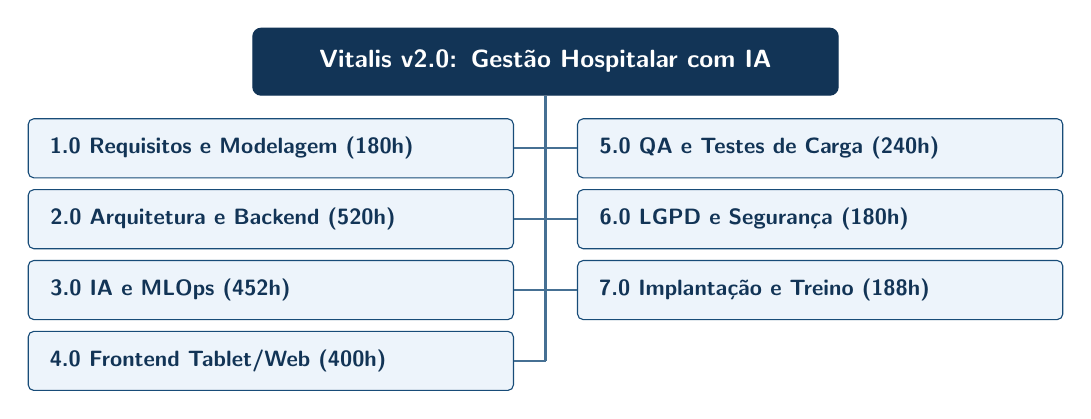
\begin{tikzpicture}[
    font=\footnotesize\sffamily,
    boxRoot/.style = {rectangle, rounded corners=3pt, draw=vitalisdark, fill=vitalisdark, text=white, font=\small\bfseries\sffamily, text width=7.2cm, align=center, minimum height=0.85cm},
    boxPkg/.style = {rectangle, rounded corners=2pt, draw=vitalisblue, fill=vitalislight!70, text=vitalisdark, font=\footnotesize\bfseries\sffamily, text width=5.6cm, align=left, minimum height=0.75cm, inner xsep=8pt},
    line/.style = {draw=vitalisblue!80, line width=0.8pt}
]
    % Nó Raiz
    \node[boxRoot] (root) at (0, 0) {Vitalis v2.0: Gestão Hospitalar com IA};

    % Tronco central
    \draw[line] (root.south) -- (0, -3.8);

    % Pacotes da Esquerda
    \node[boxPkg, anchor=east] (pkg1) at (-0.4, -1.1) {1.0 Requisitos e Modelagem (180h)};
    \node[boxPkg, anchor=east] (pkg2) at (-0.4, -2.0) {2.0 Arquitetura e Backend (520h)};
    \node[boxPkg, anchor=east] (pkg3) at (-0.4, -2.9) {3.0 IA e MLOps (452h)};
    \node[boxPkg, anchor=east] (pkg4) at (-0.4, -3.8) {4.0 Frontend Tablet/Web (400h)};

    \draw[line] (0, -1.1) -- (pkg1.east);
    \draw[line] (0, -2.0) -- (pkg2.east);
    \draw[line] (0, -2.9) -- (pkg3.east);
    \draw[line] (0, -3.8) -- (pkg4.east);

    % Pacotes da Direita
    \node[boxPkg, anchor=west] (pkg5) at (0.4, -1.1) {5.0 QA e Testes de Carga (240h)};
    \node[boxPkg, anchor=west] (pkg6) at (0.4, -2.0) {6.0 LGPD e Segurança (180h)};
    \node[boxPkg, anchor=west] (pkg7) at (0.4, -2.9) {7.0 Implantação e Treino (188h)};

    \draw[line] (0, -1.1) -- (pkg5.west);
    \draw[line] (0, -2.0) -- (pkg6.west);
    \draw[line] (0, -2.9) -- (pkg7.west);
\end{tikzpicture}
\caption{Representação hierárquica da Estrutura Analítica do Projeto (EAP)}
\label{fig:eap_vitalis}
\end{figure}

Os sete pacotes de trabalho delimitam o escopo da solução:
\begin{enumerate}[leftmargin=*]
    \item \textbf{WP 1.0: Engenharia de Requisitos e Modelagem Clínica}: Elicitação com equipes de emergência, enfermagem e faturamento, formalização dos 22 requisitos funcionais e 12 regras de negócio, modelagem de processos BPMN 2.0 e mapeamento semântico HL7 FHIR \cite{hl7_fhir:2019}.
    \item \textbf{WP 2.0: Arquitetura, Infraestrutura e Backend}: Núcleo de microsserviços em NestJS com Fastify, modelagem relacional PostgreSQL em 3NF, mensageria distribuída via BullMQ e Redis, gestão de sessões, PEP imutável, prescrição eletrônica e faturamento TISS/TUSS.
    \item \textbf{WP 3.0: Inteligência Artificial e Engenharia MLOps}: Gateway seguro com anonimização PII, pipeline de reconhecimento de fala Whisper, modelos preditivos de deterioração clínica e sepse (qSOFA/NEWS2), copiloto farmacológico RAG com \texttt{pgvector}, estimativa de permanência (LOS) e auditoria preventiva de glosas.
    \item \textbf{WP 4.0: Desenvolvimento Frontend Tablet e Web}: Design system institucional acessível (WCAG 2.1 AA), aplicação responsiva para tablets de triagem à beira do leito, mapa interativo de leitos em tempo real via WebSockets, portal web do prontuário eletrônico e portal restrito do paciente.
    \item \textbf{WP 5.0: Qualidade, Testes de Carga e Homologação}: Automação de testes unitários e de integração (Jest/Supertest), testes de ponta a ponta (Playwright), testes de carga e estresse com k6 para 2.000 conexões concorrentes e homologação clínica formal com o comitê médico.
    \item \textbf{WP 6.0: Governança, LGPD e Segurança da Informação}: Criptografia em repouso AES-256, canal seguro TLS 1.3, trilha imutável de auditoria transacional (\texttt{LOG\_AUDITORIA}), módulo de assinatura digital ICP-Brasil e análises de vulnerabilidades SAST/DAST e pentests.
    \item \textbf{WP 7.0: Implantação, Rollout e Capacitação Assistencial}: Infraestrutura como código (IaC), esteira CI/CD em Kubernetes, políticas de backup automatizado (incremental 4h e diário full), observabilidade com Prometheus e Grafana, treinamento operacional e operação assistida.
\end{enumerate}

% ==============================================================================
% 6.3 ESTIMATIVA DETALHADA POR PACOTE E SUBTAREFA
% ==============================================================================
\subsection{Estimativa Detalhada por Pacote de Trabalho e Subtarefa}

A Tabela \ref{tab:detalhamento_horas} decompõe o esforço base do projeto em 38 subtarefas de Nível 3. Cada atividade especifica o código EAP, a descrição técnica, o entregável associado, o perfil profissional responsável e a estimativa de horas de trabalho direto.

\begin{xltabular}{\textwidth}{l >{\raggedright\arraybackslash}X >{\raggedright\arraybackslash}p{4.2cm} c r}
\caption{Detalhamento de horas por pacote de trabalho e subtarefas da EAP} \label{tab:detalhamento_horas} \\
\toprule
\textbf{Cód.} & \textbf{Descrição da Subtarefa Técnica} & \textbf{Entregável Associado} & \textbf{Perfil} & \textbf{Horas} \\
\midrule
\endfirsthead

\multicolumn{5}{c}%
{{\tablename\ \thetable{}: Continuação da página anterior}} \\
\toprule
\textbf{Cód.} & \textbf{Descrição da Subtarefa Técnica} & \textbf{Entregável Associado} & \textbf{Perfil} & \textbf{Horas} \\
\midrule
\endhead

\midrule
\multicolumn{5}{r}{{Continua na próxima página \ldots}} \\
\bottomrule
\endfoot

\bottomrule
\endlastfoot

\multicolumn{5}{l}{\textit{\textbf{Pacote 1.0: Engenharia de Requisitos e Modelagem Clínica}}} \\
\midrule
1.1 & Elicitação de requisitos e entrevistas com equipe multiprofissional (médicos, enfermeiros e faturamento). & Atas de entrevistas e matriz de expectativas de stakeholders. & MED & 40 \\
\addlinespace
1.2 & Formalização da ERS (22 RFs, 12 RNs e 7 RNFs) com critérios mensuráveis de aceitação. & Documento ERS v2.0 homologado. & TL & 48 \\
\addlinespace
1.3 & Mapeamento de processos hospitalares em BPMN 2.0 (triagem, internação, prescrição e faturamento). & Modelos de processos BPMN validados. & FRONT & 36 \\
\addlinespace
1.4 & Especificação formal de Casos de Uso (UC-01 a UC-08) e elaboração da matriz de rastreabilidade. & Caderno de Casos de Uso e rastreabilidade. & BACK & 32 \\
\addlinespace
1.5 & Definição do modelo semântico de interoperabilidade clínica em conformidade com o padrão HL7 FHIR. & Especificação de perfis de recursos FHIR. & DBA & 24 \\
\midrule
\multicolumn{4}{r}{\textbf{Subtotal Pacote 1.0:}} & \textbf{180} \\
\midrule

\multicolumn{5}{l}{\textit{\textbf{Pacote 2.0: Arquitetura, Infraestrutura e Backend NestJS}}} \\
\midrule
2.1 & Desenho da arquitetura de microsserviços, Clean Architecture e gateway de integração de eventos. & Documento de Arquitetura de Software (DAS). & TL & 40 \\
\addlinespace
2.2 & Modelagem relacional em 3NF no PostgreSQL, particionamento e scripts de migração TypeORM. & DDL versionado e migrações estruturadas. & DBA & 44 \\
\addlinespace
2.3 & Módulo de autenticação, RBAC hospitalar, emissão de JWT e MFA com expiração de sessão inativa. & Microsserviço de autenticação e autorização. & BACK & 48 \\
\addlinespace
2.4 & Microsserviço de Gestão de Pacientes, Admissão e Triagem Manchester (RF-001, RF-002). & API de admissão e cálculo Manchester. & BACK & 64 \\
\addlinespace
2.5 & Microsserviço de Prontuário Eletrônico (PEP) e Evolução Clínica Estruturada (RF-005, RF-010). & API de PEP com versionamento imutável. & BACK & 80 \\
\addlinespace
2.6 & Microsserviço de Prescrição Médica Digital com checagem de alergias e regras de bloqueio (RF-006). & API de prescrição com travas farmacológicas. & BACK & 76 \\
\addlinespace
2.7 & Microsserviço de Gestão de Leitos, Alas e Higienização em tempo real via WebSockets (RF-004). & API de leitos e propagação de eventos de ala. & BACK & 60 \\
\addlinespace
2.8 & Microsserviço de Faturamento, Parametrização de Assistência e Guias TISS/TUSS (RF-007, RF-009). & API de faturamento e gerador XML TISS. & BACK & 68 \\
\addlinespace
2.9 & Mensageria assíncrona com BullMQ/Redis e barramento de eventos clínicos distribuídos. & Filas e processadores assíncronos ativos. & BACK & 40 \\
\midrule
\multicolumn{4}{r}{\textbf{Subtotal Pacote 2.0:}} & \textbf{520} \\
\midrule

\multicolumn{5}{l}{\textit{\textbf{Pacote 3.0: Inteligência Artificial e Engenharia MLOps}}} \\
\midrule
3.1 & Gateway de IA Seguro com anonimização de PII (LGPD), controle de concorrência e \textit{Circuit Breaker}. & Proxy reverso de IA com sanitização atestada. & TL & 52 \\
\addlinespace
3.2 & Pipeline de transcrição de voz para texto médico via Whisper API com vocabulário clínico normalizado. & Serviço de áudio-para-texto com WER $< 5\%$. & IA & 44 \\
\addlinespace
3.3 & Motor preditivo de deterioração clínica e detecção precoce de sepse (escores qSOFA e NEWS2). & Modelo preditivo integrado com latência $< 1{,}5\text{s}$. & IA & 68 \\
\addlinespace
3.4 & Arquitetura RAG para o Copiloto Farmacoterapêutico (Embeddings clínicos, \texttt{pgvector} e bulário). & Base vetorial e motor RAG de validação. & IA & 84 \\
\addlinespace
3.5 & Modelo preditivo de estimativa de tempo de internação (LOS) e demanda de leitos de enfermaria e UTI. & Algoritmo preditivo de ocupação de leitos. & IA & 64 \\
\addlinespace
3.6 & Módulo generativo de síntese clínica para sumários de alta e evolução estruturada (\textit{Human-in-the-Loop}). & Gerador de sumários com interface de revisão. & IA & 56 \\
\addlinespace
3.7 & Módulo de auditoria preventiva de faturamento contra glosas em guias TISS/TUSS com NLP. & Classificador de glosas e alertas de faturamento. & IA & 48 \\
\addlinespace
3.8 & Pipeline de telemetria, registro de inferências (\texttt{LOG\_INFERENCIA\_IA}) e governança médica. & Repositório de logs de inferência auditável. & DBA & 36 \\
\midrule
\multicolumn{4}{r}{\textbf{Subtotal Pacote 3.0:}} & \textbf{452} \\
\midrule

\multicolumn{5}{l}{\textit{\textbf{Pacote 4.0: Desenvolvimento Frontend Tablet e Web}}} \\
\midrule
4.1 & Design System hospitalar (Tailwind/Tokens), componentes reutilizáveis e conformidade WCAG 2.1 AA. & Biblioteca de componentes visuais acessíveis. & FRONT & 50 \\
\addlinespace
4.2 & Interface de Triagem Manchester otimizada para tablets à beira do leito (touch, formulários reativos). & Aplicação tablet para triagem de emergência. & FRONT & 64 \\
\addlinespace
4.3 & Mapa visual dinâmico de gestão de leitos com sinalização por cores e atualização via WebSockets. & Painel interativo de hotelaria hospitalar. & FRONT & 56 \\
\addlinespace
4.4 & Módulo Web de Prontuário Eletrônico (PEP) com linha do tempo clínica e prescrição rápida. & Aplicação web de atendimento médico e PEP. & FRONT & 88 \\
\addlinespace
4.5 & Componente de interface para o Copiloto de IA (alertas contextuais e justificativa médica). & Interface do copiloto com controles humanos. & FRONT & 48 \\
\addlinespace
4.6 & Dashboard administrativo com indicadores hospitalares em tempo real e exportação PDF/CSV. & Painel de telemetria e exportações gerenciais. & FRONT & 52 \\
\addlinespace
4.7 & Portal do Paciente responsivo, seguro e bilíngue (português/inglês) para consulta de laudos. & Portal do paciente homologado e acessível. & FRONT & 42 \\
\midrule
\multicolumn{4}{r}{\textbf{Subtotal Pacote 4.0:}} & \textbf{400} \\
\midrule

\multicolumn{5}{l}{\textit{\textbf{Pacote 5.0: Qualidade, Testes de Carga e Homologação}}} \\
\midrule
5.1 & Plano de garantia de qualidade (QA), matriz de cobertura e configuração de esteiras automatizadas. & Plano formal de testes e pipelines integrados. & QA & 32 \\
\addlinespace
5.2 & Implementação de testes unitários e de integração no backend com Jest e Supertest (cobertura $> 85\%$). & Bateria automatizada de testes de serviços. & QA & 64 \\
\addlinespace
5.3 & Testes de ponta a ponta (E2E) com Playwright cobrindo admissão, prescrição e faturamento. & Suíte de testes E2E executada em CI/CD. & QA & 56 \\
\addlinespace
5.4 & Testes de carga e estresse com k6 validando requisitos de desempenho (2.000 conexões, latência $< 2{,}0\text{s}$). & Relatório de validação de carga e estresse. & QA & 40 \\
\addlinespace
5.5 & Homologação clínica formal com comitê de médicos e enfermeiros (simulações assistenciais cegas). & Parecer de homologação clínica aprovado. & MED & 48 \\
\midrule
\multicolumn{4}{r}{\textbf{Subtotal Pacote 5.0:}} & \textbf{240} \\
\midrule

\multicolumn{5}{l}{\textit{\textbf{Pacote 6.0: Governança, LGPD e Segurança da Informação}}} \\
\midrule
6.1 & Diagnóstico de conformidade com a LGPD e mapeamento de fluxo de dados pessoais de saúde. & Relatório de Impacto à Proteção de Dados (RIPD). & TL & 36 \\
\addlinespace
6.2 & Implementação de criptografia AES-256 em repouso e configuração de canal TLS 1.3 em trânsito. & Mecanismo criptográfico de dados homologado. & BACK & 32 \\
\addlinespace
6.3 & Trilha de auditoria transacional imutável (\texttt{LOG\_AUDITORIA} com triggers PostgreSQL). & Mecanismo de auditoria auditado e protegido. & DBA & 36 \\
\addlinespace
6.4 & Módulo de assinatura digital padrão ICP-Brasil (PAdES / PKCS\#7) para prontuários e receitas. & Serviço de assinatura digital integrado ao CFM. & BACK & 38 \\
\addlinespace
6.5 & Análise estática (SAST), análise dinâmica (DAST) e testes de intrusão (\textit{pentests}) na API e WebSockets. & Relatório de pentest e correção de brechas. & QA & 38 \\
\midrule
\multicolumn{4}{r}{\textbf{Subtotal Pacote 6.0:}} & \textbf{180} \\
\midrule

\multicolumn{5}{l}{\textit{\textbf{Pacote 7.0: Implantação, Rollout e Capacitação Assistencial}}} \\
\midrule
7.1 & Infraestrutura como código (IaC), conteinerização Docker e orquestração de cluster Kubernetes. & Manifestos Helm/Kubernetes operacionais. & TL & 44 \\
\addlinespace
7.2 & Automação de rotinas de backup (incremental a cada 4h, diário full) e simulação de DR (RTO/RPO). & Rotinas de backup atestadas e plano de DR. & DBA & 32 \\
\addlinespace
7.3 & Configuração da pilha de observabilidade e telemetria (Prometheus, Grafana, OpenTelemetry e Loki). & Painéis de monitoramento de infraestrutura. & TL & 36 \\
\addlinespace
7.4 & Capacitação operacional e treinamento assistencial de multiplicadores (médicos, enfermagem e faturamento). & Guias de uso e certificados de capacitação. & MED & 40 \\
\addlinespace
7.5 & Operação assistida pós-lançamento (\textit{Go-Live} em ambiente controlado) e suporte de primeiro nível. & Relatório de estabilização da primeira quinzena. & QA & 36 \\
\midrule
\multicolumn{4}{r}{\textbf{Subtotal Pacote 7.0:}} & \textbf{188} \\
\midrule
\multicolumn{4}{r}{\textbf{Total Base de Esforço do Projeto (Horas):}} & \textbf{2160} \\
\end{xltabular}

% ==============================================================================
% 6.4 DISTRIBUIÇÃO DE HORAS POR PERFIL PROFISSIONAL
% ==============================================================================
\subsection{Distribuição de Horas por Perfil Profissional da Equipe}

A equipe multidisciplinar (squad) do Vitalis v2.0 conta com sete perfis profissionais especializados, cujas atribuições técnicas cobrem as demandas clínicas, arquiteturais e de qualidade:
\begin{enumerate}[leftmargin=*]
    \item \textbf{Tech Lead / Arquiteto de Software (TL)}: Responsável pelas diretrizes arquiteturais, governança de microsserviços, gateway de sanitização de IA, segurança de infraestrutura Kubernetes e esteiras de integração contínua.
    \item \textbf{Desenvolvedor Backend Sênior (DEV-BACK)}: Responsável pela implementação dos microsserviços em NestJS/Fastify, APIs RESTful, WebSockets de alta frequência, regras de negócio clínicas, PEP, prescrição eletrônica e faturamento TISS/TUSS.
    \item \textbf{Desenvolvedor Frontend / UX (DEV-FRONT)}: Responsável pela arquitetura de interface web e tablet, implementação do Design System institucional, ergonomia de telas assistenciais e conformidade de acessibilidade com WCAG 2.1 AA.
    \item \textbf{Engenheiro de IA / ML (ENG-IA)}: Responsável pela esteira de MLOps, ajuste de pipelines Whisper para áudio clínico, calibração dos motores preditivos qSOFA/NEWS2 e LOS, infraestrutura RAG com \texttt{pgvector} e integração de LLMs para síntese clínica.
    \item \textbf{DBA / Engenheiro de Dados (DBA)}: Responsável pela modelagem relacional 3NF no PostgreSQL, particionamento de tabelas de alta volumetria, indexação vetorial, integridade referencial, triggers de auditoria imutável e testes de contingência RTO/RPO.
    \item \textbf{Especialista Clínico / Consultor Médico (CONS-MED)}: Responsável pela curadoria da base de conhecimento médico, validação dos fluxos Manchester, parametrização toxicológica de prescrições, testes assistenciais cego-conduzidos e treinamento das equipes de saúde.
    \item \textbf{QA Engineer (QA)}: Responsável pela formulação da estratégia de qualidade, testes automatizados unitários e de integração, suítes ponta a ponta (E2E), simulações de carga e estresse com k6 e auditoria de vulnerabilidades de segurança.
\end{enumerate}

A Tabela \ref{tab:matriz_perfis} apresenta a matriz de distribuição de esforço multidisciplinar por pacote de trabalho da EAP e perfil profissional. Enquanto a Tabela \ref{tab:detalhamento_horas} atribui cada atividade à sua liderança técnica primária, a Tabela \ref{tab:matriz_perfis} reflete o esforço cooperativo real de todo o squad em cada frente. As somas por pacote de trabalho coincidem com os subtotais da EAP.

\begin{table}[H]
\centering
\scriptsize
\setlength{\tabcolsep}{3.5pt}
\caption{Matriz de distribuição de horas por pacote de trabalho e perfil profissional}
\label{tab:matriz_perfis}
\begin{tabularx}{\textwidth}{>{\raggedright\arraybackslash}X *{7}{>{\centering\arraybackslash}p{1.2cm}} >{\raggedleft\arraybackslash}p{1.3cm}}
\toprule
\textbf{Pacote de Trabalho (EAP)} & \textbf{TL} & \textbf{BACK} & \textbf{FRONT} & \textbf{IA} & \textbf{DBA} & \textbf{MED} & \textbf{QA} & \textbf{Total (h)} \\
\midrule
1.0 Engenharia de Requisitos e Modelagem    & 30 &  20 &  24 &  16 & 16 & 60 &  14 &  180 \\
2.0 Arquitetura, Infraestrutura e Backend   & 70 & 230 &  20 &  20 & 90 & 10 &  80 &  520 \\
3.0 Inteligência Artificial e MLOps         & 50 &  50 &  22 & 230 & 40 & 30 &  30 &  452 \\
4.0 Desenvolvimento Frontend Tablet e Web   & 30 &  30 & 250 &  10 & 10 & 20 &  50 &  400 \\
5.0 Qualidade, Testes de Carga e Homologação& 20 &  30 &  20 &  20 & 10 & 20 & 120 &  240 \\
6.0 Governança, LGPD e Segurança            & 40 &  40 &  10 &  16 & 40 & 14 &  20 &  180 \\
7.0 Implantação, Rollout e Capacitação      & 40 &  40 &  20 &  20 & 24 & 20 &  24 &  188 \\
\midrule
\textbf{Total Base por Perfil (Horas)}      & \textbf{280} & \textbf{440} & \textbf{366} & \textbf{332} & \textbf{230} & \textbf{174} & \textbf{338} & \textbf{2160} \\
\textbf{Participação Relativa no Projeto (\%)} & \textbf{12,96\%} & \textbf{20,37\%} & \textbf{16,94\%} & \textbf{15,37\%} & \textbf{10,65\%} & \textbf{8,06\%} & \textbf{15,65\%} & \textbf{100,00\%} \\
\bottomrule
\end{tabularx}
\end{table}

A distribuição de horas reflete as prioridades técnicas da arquitetura:
\begin{itemize}[leftmargin=*]
    \item \textbf{Construção de Software (Backend e Frontend)}: Soma 806 horas (37,31\% do total), dedicadas à lógica de negócio assistencial, regras clínicas e interfaces para terminais web e tablets de beira de leito.
    \item \textbf{Inteligência Artificial e Engenharia de Dados}: Concentra 562 horas (26,02\% do total), cobrindo modelos preditivos, indexação vetorial com \texttt{pgvector}, anonimização de dados pessoais e modelagem relacional 3NF.
    \item \textbf{Qualidade, Testes de Carga e Arquitetura}: Absorve 618 horas (28,61\% do total), com foco em disponibilidade de 99,9\%, tempo de resposta inferior a 2,0 segundos sob concorrência e conformidade com padrões de segurança.
    \item \textbf{Consultoria e Validação Médica}: Totaliza 174 horas (8,06\% do total), garantindo validação de fluxos Manchester, toxicologia de prescrições e treinamento das equipes de saúde.
\end{itemize}

% ==============================================================================
% 6.5 TOTAIS CONSOLIDADOS E CONTINGÊNCIA TÉCNICA
% ==============================================================================
\subsection{Totais Consolidados, Margem de Contingência e Esforço Total}

A mitigação proativa de riscos em projetos de tecnologia em saúde exige a previsão explícita de uma reserva de contingência técnica. A Tabela \ref{tab:consolidado_horas} consolida o esforço base por pacote de trabalho, detalha a reserva de contingência calculada em 15\% e totaliza as horas necessárias para o ciclo de desenvolvimento do Vitalis v2.0.

\begin{table}[H]
\centering
\small
\caption{Consolidação geral de esforço, contingência técnica e esforço total}
\label{tab:consolidado_horas}
\begin{tabularx}{\textwidth}{>{\raggedright\arraybackslash}X >{\centering\arraybackslash}p{2.3cm} >{\centering\arraybackslash}p{2.2cm} >{\centering\arraybackslash}p{2.8cm} >{\raggedleft\arraybackslash}p{2.3cm}}
\toprule
\textbf{Pacote de Trabalho (EAP)} & \textbf{Esforço Base (h)} & \textbf{Partic. (\%)} & \textbf{Contingência 15\% (h)} & \textbf{Total Projetado (h)} \\
\midrule
1.0 Engenharia de Requisitos e Modelagem    & 180  & 8,33\%  & 27,0 & 207,0 \\
2.0 Arquitetura, Infraestrutura e Backend   & 520  & 24,07\% & 78,0 & 598,0 \\
3.0 Inteligência Artificial e MLOps         & 452  & 20,93\% & 67,8 & 519,8 \\
4.0 Desenvolvimento Frontend Tablet e Web   & 400  & 18,52\% & 60,0 & 460,0 \\
5.0 Qualidade, Testes de Carga e Homologação& 240  & 11,11\% & 36,0 & 276,0 \\
6.0 Governança, LGPD e Segurança            & 180  & 8,33\%  & 27,0 & 207,0 \\
7.0 Implantação, Rollout e Capacitação      & 188  & 8,70\%  & 28,2 & 216,2 \\
\midrule
\textbf{Total Geral do Projeto Vitalis v2.0}& \textbf{2160} & \textbf{100,00\%} & \textbf{324,0} & \textbf{2484,0} \\
\bottomrule
\end{tabularx}
\end{table}

\destaqueVitalis{Síntese do Esforço e Capacidade Produtiva da Equipe Vitalis v2.0}{
    O esforço base do projeto totaliza \textbf{2.160 horas}, expandindo-se para \textbf{2.484 horas} com a incorporação da reserva de contingência técnica de 15\% (324 horas). Distribuído ao longo das \textbf{28 semanas} de desenvolvimento ativo descritas no cronograma oficial, o esforço demanda uma dedicação líquida de aproximadamente \textbf{88,7 horas por semana da equipe multidisciplinar}, plenamente compatível com a capacidade instalada do squad alocado.
}

\subsection{Viabilidade Operacional e Alinhamento com o Cronograma}

A viabilidade de execução do esforço dimensionado sustenta-se na capacidade de entrega da equipe e na estrutura das 28 semanas de cronograma:
\begin{itemize}[leftmargin=*]
    \item \textbf{Capacidade Nominal da Equipe}: Os cinco papéis com dedicação integral (Tech Lead, Backend Sênior, Frontend/UX, Engenheiro de IA e QA Engineer) operam sob regime padrão de engenharia de software de 40 horas semanais, totalizando 200 horas/semana nominais de base. Os papéis de suporte especializado (DBA / Engenheiro de Dados e Consultor Médico) operam em regime de dedicação consultiva parcial (25 horas/semana para banco de dados e 15 horas/semana para consultoria médica clínica), perfazendo uma capacidade teórica total de 240 horas semanais instaladas.
    \item \textbf{Carga de Trabalho Real vs. Capacidade}: Considerando o esforço total projetado de 2.484 horas ao longo das 28 semanas do projeto, a demanda média real corresponde a cerca de 88,7 horas/semana da equipe, o que equivale a um fator de ocupação médio em torno de 37\% da capacidade produtiva instalada total do grupo, ou 44\% considerando apenas os profissionais full-time. Essa margem oferece folga para reuniões com partes interessadas, homologações comitivas e tratamento de riscos imprevistos sem sobrecarga ou adiamento de prazos.
    \item \textbf{Sincronização com as Fases do Cronograma}: O sequenciamento acompanha as seis fases descritas na Seção 4: o esforço de requisitos (180h) e governança (180h) concentra-se nas Fases 1 e 2; o backend (520h) e frontend (400h) avançam nas Fases 2, 3 e 5; os módulos de inteligência artificial (452h) são desenvolvidos nas Fases 4 e 5; e o esforço de testes de carga, qualidade e implantação (428h) atinge o ápice nas Fases 5 e 6, finalizando com a homologação clínica na Semana 28.
\end{itemize}

\newpage

% ==============================================================================
% SEÇÃO 7: MODELAGEM DE PROCESSOS DE NEGÓCIO (BPMN 2.0)
% ==============================================================================

\section{Modelagem de Processos de Negócio (BPMN 2.0)}
\label{sec:bpmn}

A modelagem de processos em BPMN 2.0 (\textit{Business Process Model and Notation}) \cite{omg_bpmn:2011} define o encadeamento operacional, as responsabilidades de cada ator e os pontos de intervenção algorítmica no Sistema Vitalis v2.0. A formalização abrange três macroprocessos assistenciais integrados: (i) acolhimento, triagem Manchester e rastreamento preditivo de sepse; (ii) atendimento médico com copiloto clínico RAG e dispensação farmacêutica com dupla checagem; e (iii) alocação preditiva de leitos, internação, alta hospitalar e auditoria preventiva de faturamento TISS/TUSS.

% ==============================================================================
% 7.1 FUNDAMENTAÇÃO METODOLÓGICA E CONVENÇÕES BPMN
% ==============================================================================
\subsection{Fundamentação Metodológica e Notação Gráfica}
\label{subsec:bpmn_fundamentacao}

Os fluxos são estruturados em piscinas (\textit{pools}) e raias de responsabilidade (\textit{swimlanes}) que segregam os papéis de recepcionistas, enfermeiros, médicos, farmacêuticos, operadores de hotelaria e serviços automatizados de inteligência artificial.

Os diagramas adotam cinco construtos sintáticos padronizados:
\begin{itemize}[leftmargin=*]
    \item \textbf{Eventos de Início e Término (\textit{Start/End Events})}: Círculos verdes indicam o gatilho inicial do processo; círculos de borda dupla vermelha demarcam a conclusão do ciclo assistencial ou administrativo.
    \item \textbf{Tarefas de Usuário (\textit{User Tasks})}: Retângulos azuis (\texttt{bpmnTask}) representam ações executadas diretamente pelos profissionais nos terminais da plataforma.
    \item \textbf{Tarefas de IA (\textit{Service/AI Tasks})}: Retângulos roxos (\texttt{bpmnAiTask}) identificam processamentos algorítmicos autônomos, como cálculo de escores clínicos, recuperação vetorial e inferência em linguagem natural.
    \item \textbf{Desvios Exclusivos (\textit{Gateways XOR})}: Losangos laranjas (\texttt{bpmnGateway}) direcionam o controle para ramificações mutuamente excludentes segundo regras clínicas e operacionais.
    \item \textbf{Fluxos de Sequência (\textit{Sequence Flows})}: Setas direcionadas contínuas conectam os elementos na ordem estrita de execução.
\end{itemize}

\destaqueVitalis{Princípio de Supervisão Humana Estrita (\textit{Human-in-the-Loop})}{%
No Vitalis v2.0, todo componente de inteligência artificial opera como serviço de suporte consultivo à tomada de decisão clínica. Nenhum modelo preditivo ou generativo possui autoridade para prescrever intervenções terapêuticas, alterar leitos de forma compulsória ou expedir altas médicas sem a homologação formal, explícita e assinada digitalmente por profissional devidamente registrado em seu respectivo conselho de classe (CRM, COREN ou CRF).
}

% ==============================================================================
% 7.2 FLUXO 1: ACOLHIMENTO, TRIAGEM E SEPSE
% ==============================================================================
\subsection{Fluxo 1: Acolhimento, Triagem Manchester e Predição de Sepse}
\label{subsec:bpmn_fluxo1}

O primeiro fluxo modela a porta de entrada da unidade de urgência e emergência, com foco na identificação precoce de deterioração clínica e sepse. A Figura \ref{fig:bpmn_fluxo1} estrutura as atividades em quatro raias: Recepção/Acolhimento, Enfermagem/Triagem, Motor de IA Clínica e Posto Médico/Sala Vermelha.

\begin{figure}[H]
\centering
\resizebox{\textwidth}{!}{%
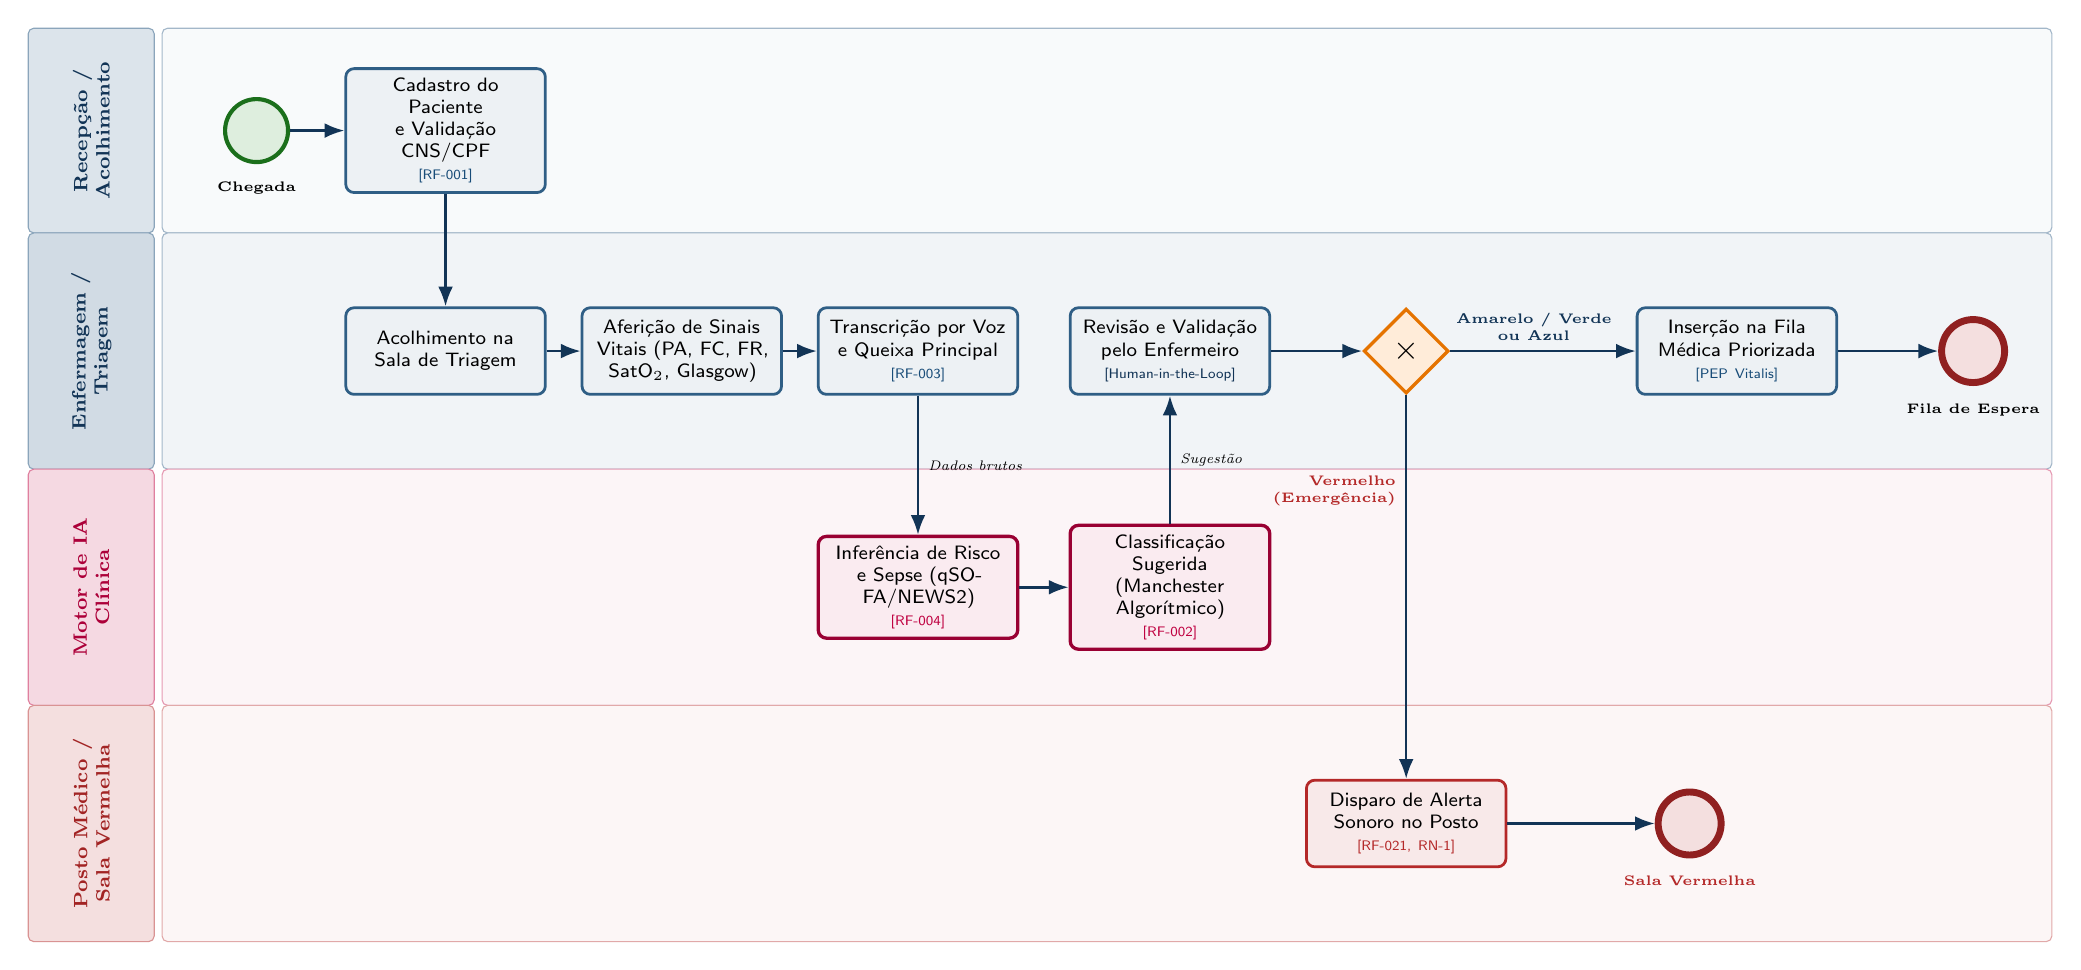
\begin{tikzpicture}[node distance=1.5cm, font=\sffamily]
  % Raias de Responsabilidade (Swimlanes)
  \draw[vitalisblue!40, fill=vitalisblue!3, rounded corners=2pt] (-0.8, 6.8) rectangle (23.2, 9.4);
  \draw[vitalisblue!40, fill=vitalisblue!6, rounded corners=2pt] (-0.8, 3.8) rectangle (23.2, 6.8);
  \draw[purple!40, fill=purple!4, rounded corners=2pt] (-0.8, 0.8) rectangle (23.2, 3.8);
  \draw[vitalisred!40, fill=vitalisred!4, rounded corners=2pt] (-0.8, -2.2) rectangle (23.2, 0.8);

  % Cabeçalhos das Raias (Faixas Laterais)
  \draw[vitalisblue!50, fill=vitalisblue!15, rounded corners=2pt] (-2.5, 6.8) rectangle (-0.9, 9.4);
  \draw[vitalisblue!50, fill=vitalisblue!20, rounded corners=2pt] (-2.5, 3.8) rectangle (-0.9, 6.8);
  \draw[purple!50, fill=purple!15, rounded corners=2pt] (-2.5, 0.8) rectangle (-0.9, 3.8);
  \draw[vitalisred!50, fill=vitalisred!15, rounded corners=2pt] (-2.5, -2.2) rectangle (-0.9, 0.8);

  % Identificação das Raias
  \node[rotate=90, text=vitalisdark, font=\bfseries\scriptsize, align=center] at (-1.7, 8.1) {Recepção /\\Acolhimento};
  \node[rotate=90, text=vitalisdark, font=\bfseries\scriptsize, align=center] at (-1.7, 5.3) {Enfermagem /\\Triagem};
  \node[rotate=90, text=purple!90!black, font=\bfseries\scriptsize, align=center] at (-1.7, 2.3) {Motor de IA\\Clínica};
  \node[rotate=90, text=vitalisred!90!black, font=\bfseries\scriptsize, align=center] at (-1.7, -0.7) {Posto Médico /\\Sala Vermelha};

  % Nós de Atividade e Eventos
  \node[bpmnStart] (start1) at (0.4, 8.1) {};
  \node[font=\tiny\bfseries, below=1mm of start1] {Chegada};

  \node[bpmnTask] (t_cad) at (2.8, 8.1) {Cadastro do Paciente\\e Validação CNS/CPF\\{\tiny\color{vitalisblue}[RF-001]}};
  
  \node[bpmnTask] (t_sala) at (2.8, 5.3) {Acolhimento na\\Sala de Triagem};

  \node[bpmnTask] (t_vitais) at (5.8, 5.3) {Aferição de Sinais\\Vitais (PA, FC, FR,\\SatO$_2$, Glasgow)};

  \node[bpmnTask] (t_voz) at (8.8, 5.3) {Transcrição por Voz\\e Queixa Principal\\{\tiny\color{vitalisblue}[RF-003]}};

  \node[bpmnAiTask] (t_sepse) at (8.8, 2.3) {Inferência de Risco\\e Sepse (qSOFA/NEWS2)\\{\tiny\color{purple}[RF-004]}};

  \node[bpmnAiTask] (t_manch) at (12.0, 2.3) {Classificação Sugerida\\(Manchester Algorítmico)\\{\tiny\color{purple}[RF-002]}};

  \node[bpmnTask] (t_val) at (12.0, 5.3) {Revisão e Validação\\pelo Enfermeiro\\{\tiny\color{vitalisdark}[Human-in-the-Loop]}};

  \node[bpmnGateway] (gw_grav) at (15.0, 5.3) {\bfseries\large $\times$};

  % Ramo Vermelho (Emergência Absoluta)
  \node[bpmnTask, draw=vitalisred, fill=vitalisred!10] (t_emerg) at (15.0, -0.7) {Disparo de Alerta\\Sonoro no Posto\\{\tiny\color{vitalisred}[RF-021, RN-1]}};
  \node[bpmnEnd] (end_emerg) at (18.6, -0.7) {};
  \node[font=\tiny\bfseries\color{vitalisred}, below=1mm of end_emerg] {Sala Vermelha};

  % Ramo Demais Cores (Fila Ordinária Priorizada)
  \node[bpmnTask] (t_fila) at (19.2, 5.3) {Inserção na Fila\\Médica Priorizada\\{\tiny\color{vitalisblue}[PEP Vitalis]}};
  \node[bpmnEnd] (end_fila) at (22.2, 5.3) {};
  \node[font=\tiny\bfseries, below=1mm of end_fila] {Fila de Espera};

  % Conexões Ortogonais
  \draw[bpmnArrow] (start1) -- (t_cad);
  \draw[bpmnArrow] (t_cad) -- (t_sala);
  \draw[bpmnArrow] (t_sala) -- (t_vitais);
  \draw[bpmnArrow] (t_vitais) -- (t_voz);
  \draw[bpmnArrow] (t_voz) -- node[right, font=\tiny\itshape] {Dados brutos} (t_sepse);
  \draw[bpmnArrow] (t_sepse) -- (t_manch);
  \draw[bpmnArrow] (t_manch) -- node[right, font=\tiny\itshape] {Sugestão} (t_val);
  \draw[bpmnArrow] (t_val) -- (gw_grav);

  \draw[bpmnArrow] (gw_grav) -- node[left, align=right, pos=0.25, font=\tiny\bfseries\color{vitalisred}] {Vermelho\\(Emergência)} (t_emerg);
  \draw[bpmnArrow] (t_emerg) -- (end_emerg);

  \draw[bpmnArrow] (gw_grav) -- node[above, align=center, pos=0.45, font=\tiny\bfseries\color{vitalisdark}] {Amarelo / Verde\\ou Azul} (t_fila);
  \draw[bpmnArrow] (t_fila) -- (end_fila);
\end{tikzpicture}%
}
\caption{Fluxo BPMN 1: Acolhimento, Triagem Manchester e Predição de Sepse no Vitalis v2.0.}
\label{fig:bpmn_fluxo1}
\end{figure}

O fluxo compreende as seguintes etapas sequenciais:
\begin{enumerate}[leftmargin=*]
    \item \textbf{Identificação Cadastral do Paciente}: Na recepção, o atendente registra os dados básicos e valida o número do Cartão Nacional de Saúde (CNS) e CPF em barramento oficial, gerando o identificador unificado de atendimento (RF-001).
    \item \textbf{Acolhimento e Coleta de Sinais Vitais}: O paciente é direcionado à sala de triagem. O enfermeiro afere pressão arterial sistólica e diastólica (PA), frequência cardíaca (FC), frequência respiratória (FR), saturação periférica de oxigênio ($\text{SatO}_2$), temperatura axilar e nível de consciência pela escala de coma de Glasgow.
    \item \textbf{Transcrição de Voz com PLN}: Paralelamente ao exame físico, o profissional narra a queixa principal e o histórico recente. O módulo de transcrição converte o áudio em texto estruturado com latência inferior a $2{,}0\,\text{s}$ (RF-003).
    \item \textbf{Inferência Preditiva de Sepse e Deterioração}: Os dados fisiológicos alimentam o motor de inteligência artificial, que calcula simultaneamente os escores qSOFA e NEWS2 \cite{singer_sepsis:2016} (RF-004), identificando sinais precoces de resposta inflamatória sistêmica antes do choque clínico manifesto.
    \item \textbf{Sugestão Manchester e Validação Humana}: O algoritmo de triagem projeta a classificação recomendada conforme a árvore de decisão do Protocolo de Manchester \cite{manchester:2014} (RF-002). O enfermeiro avalia o quadro global do paciente, podendo chancelar a recomendação ou elevar a categoria de risco caso constate fatores atípicos não capturados pelos sensores (Regra de Negócio RN-1).
    \item \textbf{Desvio de Gravidade e Conduta Imediata}:
    \begin{itemize}
        \item \textit{Classificação Vermelha (Emergência)}: O sistema emite alerta sonoro no posto médico, exibe notificação visual de bloqueio (RF-021) e mobiliza a equipe para encaminhamento imediato do paciente ao leito de estabilização (sala vermelha), com atendimento imediato.
        \item \textit{Classificações Laranja, Amarela, Verde e Azul}: O atendimento é posicionado na lista médica do prontuário eletrônico com ordenação decrescente por gravidade clínica e tempo decorrido, respeitando os tempos máximos de espera do protocolo.
    \end{itemize}
\end{enumerate}

% ==============================================================================
% 7.3 FLUXO 2: ATENDIMENTO MÉDICO, RAG E DISPENSAÇÃO
% ==============================================================================
\subsection{Fluxo 2: Atendimento Médico, Copiloto RAG e Dispensação Farmacêutica}
\label{subsec:bpmn_fluxo2}

O segundo fluxo integra a prescrição médica, a análise farmacológica apoiada por inteligência artificial e a dispensação de beira de leito. A modelagem na Figura \ref{fig:bpmn_fluxo2} organiza o fluxo em três raias: Médico Assistente (PEP), Copiloto de IA Clínico e Farmácia Satélite/Leito.

\begin{figure}[H]
\centering
\resizebox{\textwidth}{!}{%
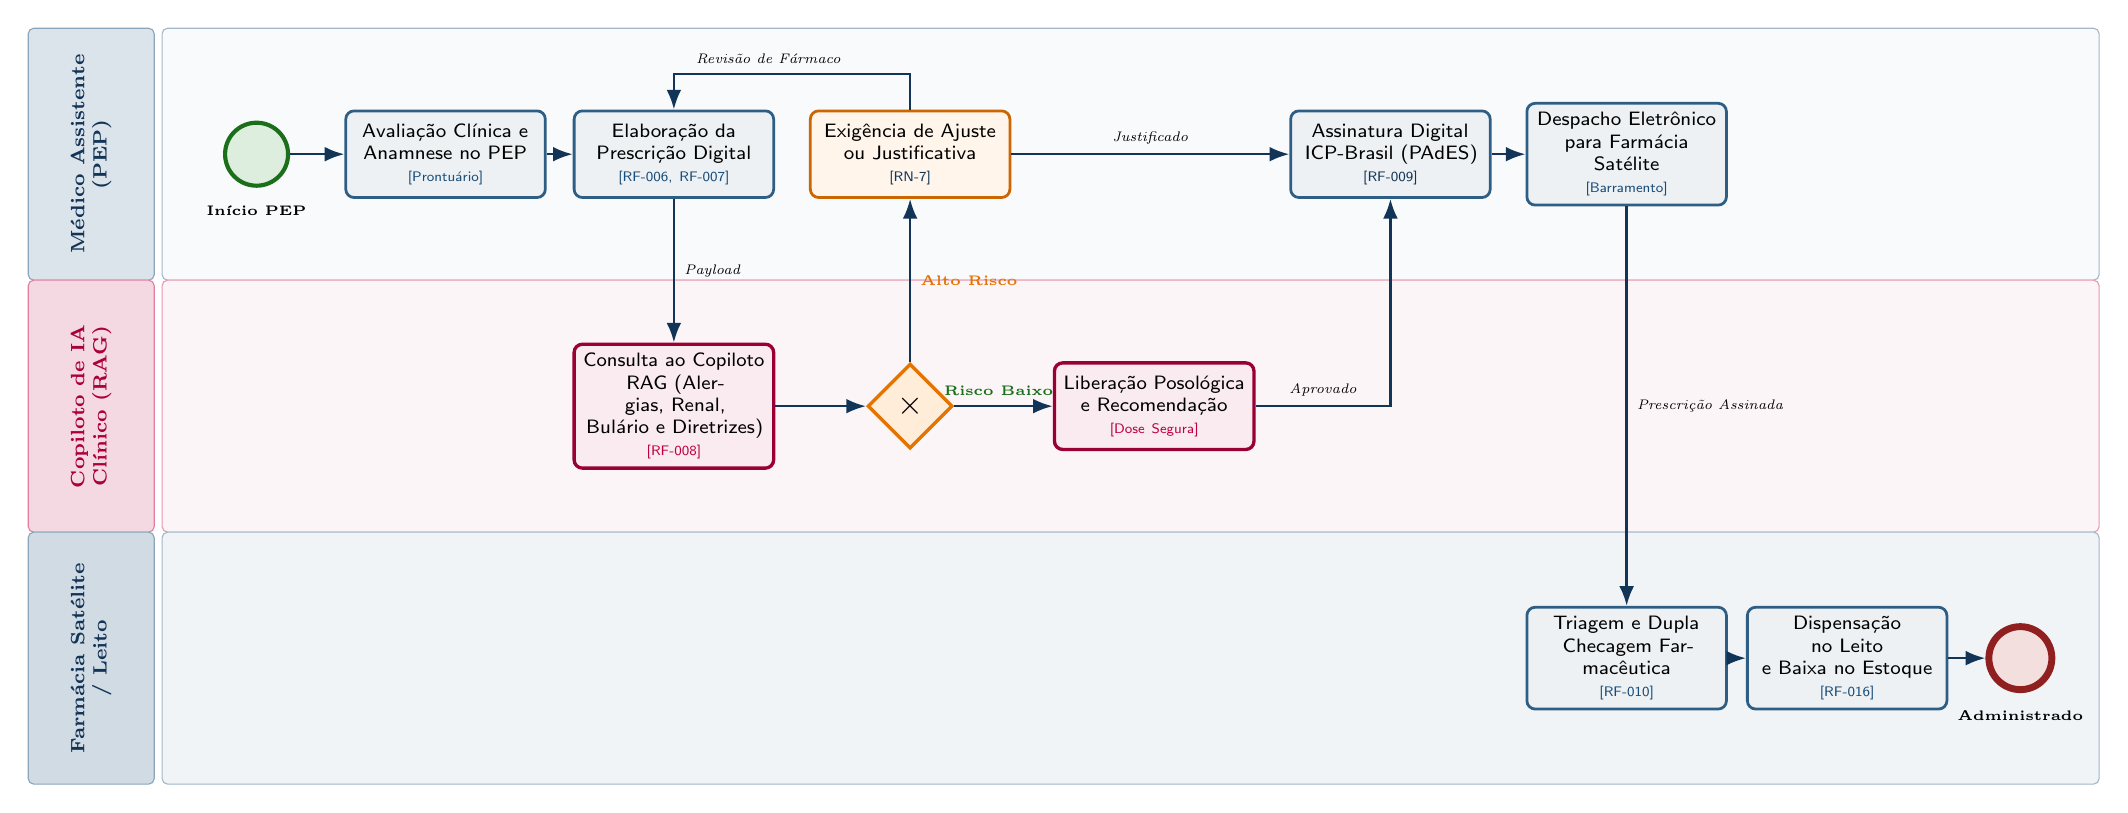
\begin{tikzpicture}[node distance=1.5cm, font=\sffamily]
  % Raias de Responsabilidade (Swimlanes)
  \draw[vitalisblue!40, fill=vitalisblue!3, rounded corners=2pt] (-0.8, 4.0) rectangle (23.8, 7.2);
  \draw[purple!40, fill=purple!4, rounded corners=2pt] (-0.8, 0.8) rectangle (23.8, 4.0);
  \draw[vitalisblue!40, fill=vitalisblue!6, rounded corners=2pt] (-0.8, -2.4) rectangle (23.8, 0.8);

  % Cabeçalhos das Raias (Faixas Laterais)
  \draw[vitalisblue!50, fill=vitalisblue!15, rounded corners=2pt] (-2.5, 4.0) rectangle (-0.9, 7.2);
  \draw[purple!50, fill=purple!15, rounded corners=2pt] (-2.5, 0.8) rectangle (-0.9, 4.0);
  \draw[vitalisblue!50, fill=vitalisblue!20, rounded corners=2pt] (-2.5, -2.4) rectangle (-0.9, 0.8);

  % Identificação das Raias
  \node[rotate=90, text=vitalisdark, font=\bfseries\scriptsize, align=center] at (-1.7, 5.6) {Médico Assistente\\(PEP)};
  \node[rotate=90, text=purple!90!black, font=\bfseries\scriptsize, align=center] at (-1.7, 2.4) {Copiloto de IA\\Clínico (RAG)};
  \node[rotate=90, text=vitalisdark, font=\bfseries\scriptsize, align=center] at (-1.7, -0.8) {Farmácia Satélite\\/ Leito};

  % Nós de Atividade e Eventos
  \node[bpmnStart] (start2) at (0.4, 5.6) {};
  \node[font=\tiny\bfseries, below=1mm of start2] {Início PEP};

  \node[bpmnTask] (t_aval) at (2.8, 5.6) {Avaliação Clínica e\\Anamnese no PEP\\{\tiny\color{vitalisblue}[Prontuário]}};
  \node[bpmnTask] (t_presc) at (5.7, 5.6) {Elaboração da\\Prescrição Digital\\{\tiny\color{vitalisblue}[RF-006, RF-007]}};

  \node[bpmnAiTask] (t_rag) at (5.7, 2.4) {Consulta ao Copiloto\\RAG (Alergias, Renal,\\Bulário e Diretrizes)\\{\tiny\color{purple}[RF-008]}};
  
  \node[bpmnGateway] (gw_inter) at (8.7, 2.4) {\bfseries\large $\times$};

  \node[bpmnTask, draw=orange!80!black, fill=orange!8] (t_just) at (8.7, 5.6) {Exigência de Ajuste\\ou Justificativa\\{\tiny\color{vitalisdark}[RN-7]}};

  \node[bpmnAiTask] (t_lib) at (11.8, 2.4) {Liberação Posológica\\e Recomendação\\{\tiny\color{purple}[Dose Segura]}};

  \node[bpmnTask] (t_assina) at (14.8, 5.6) {Assinatura Digital\\ICP-Brasil (PAdES)\\{\tiny\color{vitalisdark}[RF-009]}};

  \node[bpmnTask] (t_desp) at (17.8, 5.6) {Despacho Eletrônico\\para Farmácia Satélite\\{\tiny\color{vitalisblue}[Barramento]}};

  \node[bpmnTask] (t_farm) at (17.8, -0.8) {Triagem e Dupla\\Checagem Farmacêutica\\{\tiny\color{vitalisblue}[RF-010]}};

  \node[bpmnTask] (t_disp) at (20.6, -0.8) {Dispensação no Leito\\e Baixa no Estoque\\{\tiny\color{vitalisblue}[RF-016]}};

  \node[bpmnEnd] (end2) at (22.8, -0.8) {};
  \node[font=\tiny\bfseries, below=1mm of end2] {Administrado};

  % Conexões Ortogonais
  \draw[bpmnArrow] (start2) -- (t_aval);
  \draw[bpmnArrow] (t_aval) -- (t_presc);
  \draw[bpmnArrow] (t_presc) -- node[right, font=\tiny\itshape] {Payload} (t_rag);
  \draw[bpmnArrow] (t_rag) -- (gw_inter);

  \draw[bpmnArrow] (gw_inter) -- node[right, font=\tiny\bfseries\color{orange!90!black}] {Alto Risco} (t_just);
  \draw[bpmnArrow] (t_just.north) -- ++(0, 0.45) -| node[above, pos=0.3, font=\tiny\itshape] {Revisão de Fármaco} (t_presc.north);
  \draw[bpmnArrow] (t_just) -- node[above, font=\tiny\itshape] {Justificado} (t_assina);

  \draw[bpmnArrow] (gw_inter) -- node[above, pos=0.45, font=\tiny\bfseries\color{vitalisgreen!80!black}] {Risco Baixo} (t_lib);
  \draw[bpmnArrow] (t_lib.east) -| node[above, pos=0.25, font=\tiny\itshape] {Aprovado} (t_assina.south);

  \draw[bpmnArrow] (t_assina) -- (t_desp);
  \draw[bpmnArrow] (t_desp) -- node[right, font=\tiny\itshape] {Prescrição Assinada} (t_farm);
  \draw[bpmnArrow] (t_farm) -- (t_disp);
  \draw[bpmnArrow] (t_disp) -- (end2);
\end{tikzpicture}%
}
\caption{Fluxo BPMN 2: Atendimento Médico, Copiloto RAG e Dispensação Farmacêutica no Vitalis v2.0.}
\label{fig:bpmn_fluxo2}
\end{figure}

O ciclo de prescrição e dispensação é estruturado nos seguintes passos:
\begin{enumerate}[leftmargin=*]
    \item \textbf{Abertura do PEP e Exame Clínico}: O médico assistente acessa o prontuário do paciente, registrando as queixas evolutivas, achados do exame físico e a hipótese diagnóstica.
    \item \textbf{Composição da Prescrição Digital}: O profissional seleciona os fármacos, dosagens, diluições, vias de administração e intervalos posológicos via catálogo estruturado (RF-006, RF-007).
    \item \textbf{Interrogação do Copiloto RAG de Farmacologia}: Conforme os medicamentos são adicionados, o sistema despacha os identificadores farmacológicos ao serviço de inteligência artificial. O modelo realiza busca semântica em bulários oficiais da ANVISA e diretrizes hospitalares \cite{lewis_rag:2020} (RF-008), cruzando os dados com histórico de alergias, \textit{clearance} de creatinina (função renal) e marcadores de função hepática.
    \item \textbf{Gateway de Interação Medicamentosa}:
    \begin{itemize}
        \item \textit{Risco Alto ou Contraindicação Formal}: O sistema suspende a confirmação direta da prescrição, exibe as notas técnicas que fundamentam a restrição e exige substituição do fármaco ou registro de justificativa técnica no prontuário (Regra RN-7).
        \item \textit{Risco Baixo ou Posologia Compatível}: O copiloto valida os parâmetros e libera a receita para validação documental.
    \end{itemize}
    \item \textbf{Assinatura Digital Padrão ICP-Brasil}: O médico assina o documento nos padrões PAdES e PKCS\#7 com carimbo do tempo, atendendo à Resolução CFM nº 2.299/2021 \cite{cfm_digital:2021} (RF-009).
    \item \textbf{Despacho e Triagem na Farmácia Satélite}: A prescrição assinada é transmitida eletronicamente à farmácia da respectiva ala. O farmacêutico confere os itens e executa a dupla checagem dos medicamentos de alta vigilância antes do fracionamento (RF-010).
    \item \textbf{Dispensação Beira-Leito e Baixa Automática}: No posto de internação, a enfermagem realiza a checagem cruzada da pulseira do paciente e do código de barras do medicamento. A confirmação registra a administração e decrementa o saldo de estoque (RF-016), mantendo a rastreabilidade do lote.
\end{enumerate}

% ==============================================================================
% 7.4 FLUXO 3: LEITOS, ALTA E TISS/TUSS
% ==============================================================================
\subsection{Fluxo 3: Alocação Preditiva de Leitos, Evolução, Alta e Auditoria TISS/TUSS}
\label{subsec:bpmn_fluxo3}

O terceiro fluxo abrange a gestão de internação, a alocação dinâmica de capacidade instalada e a governança de faturamento hospitalar. O Vitalis v2.0 combina predição de tempo de internação (\textit{Length of Stay}, LOS), sumarização clínica de alta por modelos de linguagem e auditoria preventiva segundo o padrão TISS da ANS \cite{ans_tiss:2023}. A Figura \ref{fig:bpmn_fluxo3} apresenta as etapas do processo.

\begin{figure}[H]
\centering
\resizebox{\textwidth}{!}{%
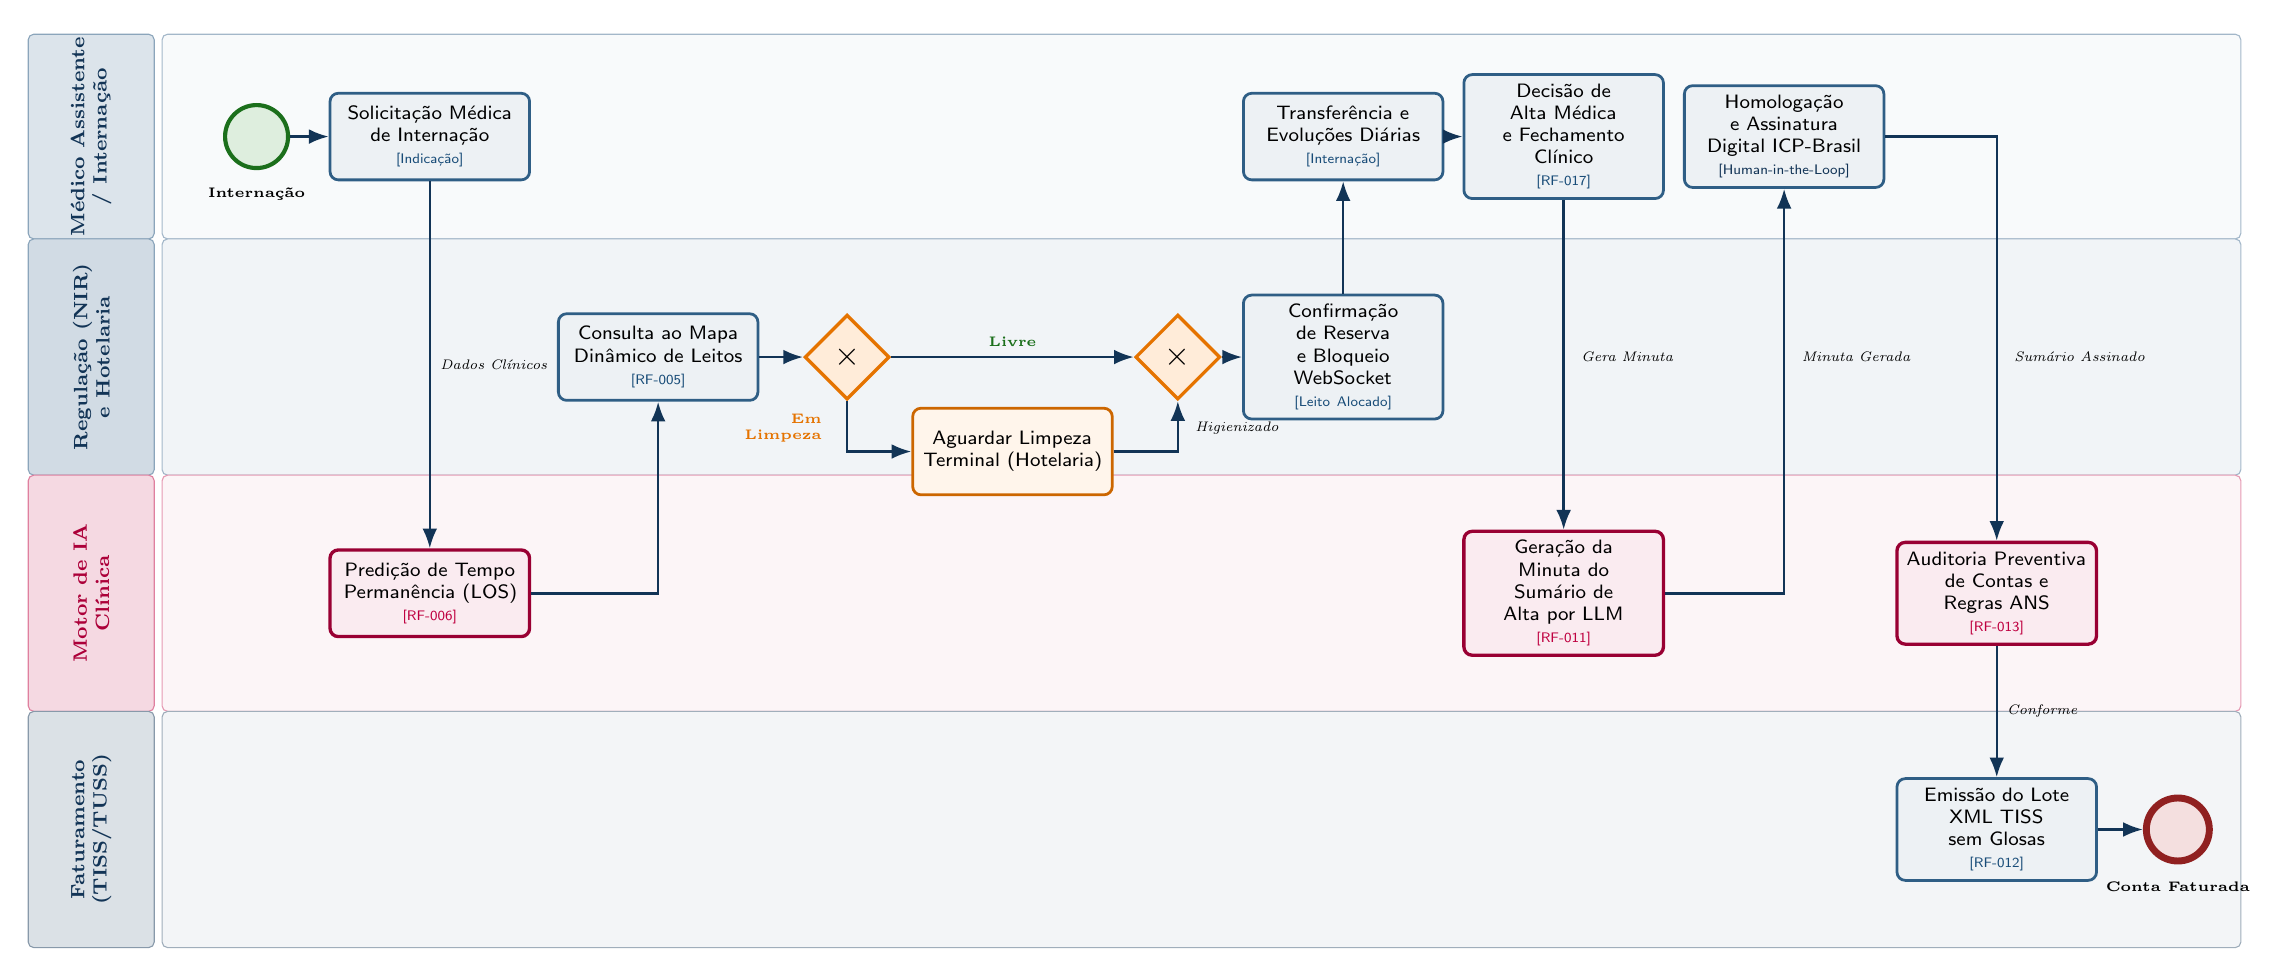
\begin{tikzpicture}[node distance=1.5cm, font=\sffamily]
  % Raias de Responsabilidade (Swimlanes)
  \draw[vitalisblue!40, fill=vitalisblue!3, rounded corners=2pt] (-0.8, 6.8) rectangle (25.6, 9.4);
  \draw[vitalisblue!40, fill=vitalisblue!6, rounded corners=2pt] (-0.8, 3.8) rectangle (25.6, 6.8);
  \draw[purple!40, fill=purple!4, rounded corners=2pt] (-0.8, 0.8) rectangle (25.6, 3.8);
  \draw[vitalisdark!40, fill=vitalisdark!5, rounded corners=2pt] (-0.8, -2.2) rectangle (25.6, 0.8);

  % Cabeçalhos das Raias (Faixas Laterais)
  \draw[vitalisblue!50, fill=vitalisblue!15, rounded corners=2pt] (-2.5, 6.8) rectangle (-0.9, 9.4);
  \draw[vitalisblue!50, fill=vitalisblue!20, rounded corners=2pt] (-2.5, 3.8) rectangle (-0.9, 6.8);
  \draw[purple!50, fill=purple!15, rounded corners=2pt] (-2.5, 0.8) rectangle (-0.9, 3.8);
  \draw[vitalisdark!50, fill=vitalisdark!15, rounded corners=2pt] (-2.5, -2.2) rectangle (-0.9, 0.8);

  % Identificação das Raias
  \node[rotate=90, text=vitalisdark, font=\bfseries\scriptsize, align=center] at (-1.7, 8.1) {Médico Assistente\\/ Internação};
  \node[rotate=90, text=vitalisdark, font=\bfseries\scriptsize, align=center] at (-1.7, 5.3) {Regulação (NIR)\\e Hotelaria};
  \node[rotate=90, text=purple!90!black, font=\bfseries\scriptsize, align=center] at (-1.7, 2.3) {Motor de IA\\Clínica};
  \node[rotate=90, text=vitalisdark, font=\bfseries\scriptsize, align=center] at (-1.7, -0.7) {Faturamento\\(TISS/TUSS)};

  % Nós de Atividade e Eventos
  \node[bpmnStart] (start3) at (0.4, 8.1) {};
  \node[font=\tiny\bfseries, below=1mm of start3] {Internação};

  \node[bpmnTask] (t_solic) at (2.6, 8.1) {Solicitação Médica\\de Internação\\{\tiny\color{vitalisblue}[Indicação]}};

  \node[bpmnAiTask] (t_los) at (2.6, 2.3) {Predição de Tempo\\Permanência (LOS)\\{\tiny\color{purple}[RF-006]}};

  \node[bpmnTask] (t_mapa) at (5.5, 5.3) {Consulta ao Mapa\\Dinâmico de Leitos\\{\tiny\color{vitalisblue}[RF-005]}};

  \node[bpmnGateway] (gw_leito) at (7.9, 5.3) {\bfseries\large $\times$};

  \node[bpmnTask, draw=orange!80!black, fill=orange!8] (t_limpeza) at (10.0, 4.1) {Aguardar Limpeza\\Terminal (Hotelaria)};

  \node[bpmnGateway] (gw_join) at (12.1, 5.3) {\bfseries\large $\times$};

  \node[bpmnTask] (t_reserva) at (14.2, 5.3) {Confirmação de Reserva\\e Bloqueio WebSocket\\{\tiny\color{vitalisblue}[Leito Alocado]}};

  \node[bpmnTask] (t_transf) at (14.2, 8.1) {Transferência e\\Evoluções Diárias\\{\tiny\color{vitalisblue}[Internação]}};

  \node[bpmnTask] (t_alta) at (17.0, 8.1) {Decisão de Alta Médica\\e Fechamento Clínico\\{\tiny\color{vitalisblue}[RF-017]}};

  \node[bpmnAiTask] (t_llm) at (17.0, 2.3) {Geração da Minuta do\\Sumário de Alta por LLM\\{\tiny\color{purple}[RF-011]}};

  \node[bpmnTask] (t_homolog) at (19.8, 8.1) {Homologação e Assinatura\\Digital ICP-Brasil\\{\tiny\color{vitalisdark}[Human-in-the-Loop]}};

  \node[bpmnAiTask] (t_audit) at (22.5, 2.3) {Auditoria Preventiva\\de Contas e Regras ANS\\{\tiny\color{purple}[RF-013]}};

  \node[bpmnTask] (t_tiss) at (22.5, -0.7) {Emissão do Lote\\XML TISS sem Glosas\\{\tiny\color{vitalisblue}[RF-012]}};

  \node[bpmnEnd] (end3) at (24.8, -0.7) {};
  \node[font=\tiny\bfseries, below=1mm of end3] {Conta Faturada};

  % Conexões Ortogonais
  \draw[bpmnArrow] (start3) -- (t_solic);
  \draw[bpmnArrow] (t_solic) -- node[right, font=\tiny\itshape] {Dados Clínicos} (t_los);
  \draw[bpmnArrow] (t_los.east) -| (t_mapa.south);
  \draw[bpmnArrow] (t_mapa) -- (gw_leito);

  \draw[bpmnArrow] (gw_leito.south) |- (t_limpeza.west);
  \node[left, align=right, font=\tiny\bfseries\color{orange!90!black}] at (7.7, 4.4) {Em\\Limpeza};

  \draw[bpmnArrow] (t_limpeza.east) -| (gw_join.south);
  \node[right, font=\tiny\itshape] at (12.2, 4.4) {Higienizado};

  \draw[bpmnArrow] (gw_leito) -- node[above, font=\tiny\bfseries\color{vitalisgreen!80!black}] {Livre} (gw_join);
  \draw[bpmnArrow] (gw_join) -- (t_reserva);

  \draw[bpmnArrow] (t_reserva) -- (t_transf);
  \draw[bpmnArrow] (t_transf) -- (t_alta);
  
  \draw[bpmnArrow] (t_alta) -- (t_llm);
  \node[right, font=\tiny\itshape] at (17.1, 5.3) {Gera Minuta};

  \draw[bpmnArrow] (t_llm.east) -| (t_homolog.south);
  \node[right, font=\tiny\itshape] at (19.9, 5.3) {Minuta Gerada};

  \draw[bpmnArrow] (t_homolog.east) -| (t_audit.north);
  \node[right, font=\tiny\itshape] at (22.6, 5.3) {Sumário Assinado};

  \draw[bpmnArrow] (t_audit) -- node[right, font=\tiny\itshape] {Conforme} (t_tiss);
  \draw[bpmnArrow] (t_tiss) -- (end3);
\end{tikzpicture}%
}
\caption{Fluxo BPMN 3: Alocação Preditiva de Leitos, Evolução, Alta e Auditoria TISS/TUSS no Vitalis v2.0.}
\label{fig:bpmn_fluxo3}
\end{figure}

As etapas constitutivas deste fluxo compreendem:
\begin{enumerate}[leftmargin=*]
    \item \textbf{Indicação Médica de Internação}: O médico assistente conclui que o quadro clínico requer leito hospitalar e registra o pedido no prontuário com CID-10 e justificativa.
    \item \textbf{Predição de Tempo de Permanência (LOS)}: O modelo de IA processa o perfil clínico do paciente, comorbidades e faixa etária, projetando a estimativa de dias de internação e nível de cuidados (RF-006).
    \item \textbf{Consulta ao Mapa Dinâmico de Leitos}: O Núcleo Interno de Regulação (NIR) consulta a disponibilidade de vagas em tempo real (RF-005) em enfermarias, leitos semi-intensivos ou UTI.
    \item \textbf{Gateway de Ocupação e Higienização}:
    \begin{itemize}
        \item \textit{Leito em Higienização ou Manutenção}: O sistema emite ordem de serviço para limpeza terminal pela hotelaria hospitalar. O paciente aguarda em observação transitória até a liberação física do quarto.
        \item \textit{Leito Livre}: O NIR confirma a alocação e bloqueia o leito instantaneamente via conexões WebSocket.
    \end{itemize}
    \item \textbf{Transferência e Registro de Evoluções Clínicas}: O paciente é admitido no leito designado. A equipe multidisciplinar registra evoluções diárias, aprazamentos de enfermagem e resultados de exames complementares.
    \item \textbf{Decisão de Alta Médica e Minuta por LLM}: Finalizado o plano terapêutico, o médico prescreve a alta no sistema (RF-017). O modelo de linguagem processa o prontuário da internação e redige uma minuta estruturada de sumário de alta em menos de $3{,}0\,\text{s}$ (RF-011).
    \item \textbf{Homologação Médica e Auditoria Preventiva ANS}: O médico revisa a minuta, realiza eventuais ajustes e assina digitalmente com certificado ICP-Brasil (\textit{Human-in-the-Loop}). O motor de auditoria analisa a conta hospitalar, confrontando os itens cobrados com tabelas TUSS, guias de autorização e contratos com operadoras (RF-013).
    \item \textbf{Emissão do Lote XML TISS}: Confirmada a conformidade documental, o faturamento compila o lote XML no padrão TISS sem glosas (RF-012) e encerra a conta contábil do atendimento.
\end{enumerate}

% ==============================================================================
% 7.5 MATRIZ COMPARATIVA DE PROCESSOS, ATORES E IA
% ==============================================================================
\subsection{Matriz de Atores, Intervenções de IA e Salvaguardas}
\label{subsec:bpmn_matriz}

A Tabela \ref{tab:matriz_bpmn} resume os papéis operacionais, as intervenções de IA e os mecanismos de governança humana em cada macroprocesso assistencial.

\begin{table}[H]
\centering
\small
\renewcommand{\arraystretch}{1.2}
\begin{tabularx}{\textwidth}{>{\raggedright\arraybackslash}p{2.8cm} >{\raggedright\arraybackslash}p{2.8cm} >{\raggedright\arraybackslash}p{4.6cm} >{\raggedright\arraybackslash}X}
\toprule
\textbf{Fluxo Assistencial} & \textbf{Atores} & \textbf{Intervenção de IA} & \textbf{Salvaguarda de Governança} \\
\midrule
\textbf{Fluxo 1:}\newline Acolhimento e Sepse &
Recepcionista,\newline Enfermeiro Triador,\newline Médico de Urgência. &
Transcrição de voz em tempo real (RF-003), cálculo preditivo de sepse via qSOFA/NEWS2 (RF-004) e recomendação de cor Manchester (RF-002). &
O enfermeiro avalia presencialmente o paciente e possui autonomia para manter ou elevar a classificação de gravidade (RN-1). \\
\midrule
\textbf{Fluxo 2:}\newline Consulta e Farmácia &
Médico Assistente,\newline Farmacêutico,\newline Enfermeiro de Leito. &
Recuperação via RAG para checagem de interações medicamentosas, ajuste por função renal/hepática e bulários (RF-008). &
Prescrição exclusiva do médico com assinatura ICP-Brasil (RF-009) e justificativa obrigatória para alertas de alto risco (RN-7). Dupla checagem biométrica na dispensação (RF-010). \\
\midrule
\textbf{Fluxo 3:}\newline Leitos, Alta e Faturamento &
Médico Assistente,\newline Analista do NIR,\newline Hotelaria Hospitalar,\newline Faturista. &
Predição de tempo de permanência hospitalar LOS (RF-006), minuta do sumário de alta por LLM (RF-011) e auditoria preventiva ANS (RF-013). &
Internação e alta decididas pelo médico assistente, com assinatura digital no sumário (RF-017). Fechamento do lote validado pela equipe de faturamento (RF-012). \\
\bottomrule
\end{tabularx}
\caption{Matriz de Atores, Intervenções de IA e Salvaguardas dos Processos BPMN.}
\label{tab:matriz_bpmn}
\end{table}

A modelagem BPMN apresentada confere rastreabilidade técnica e rigor operacional ao Vitalis v2.0, assegurando que o emprego de inteligência artificial eleve a segurança clínica sem comprometer a primazia decisória dos profissionais de saúde.

\newpage

% ==============================================================================
% SEÇÃO 8: DIAGRAMA DE CLASSES UML DO SISTEMA VITALIS v2.0
% ==============================================================================

\section{Diagrama de Classes UML do Sistema Vitalis v2.0}
\label{sec:diagrama_classes}

A modelagem estrutural de um ambiente de missão crítica como o Sistema de Gestão Hospitalar Inteligente Vitalis (Versão 2.0) exige rigor conceitual e alta fidelidade entre a lógica de negócios assistencial e a persistência relacional. Em hospitais gerais e terciários, falhas na integridade de dados podem ocasionar decisões clínicas equivocadas, atrasos terapêuticos e sanções legais severas \cite{sommerville:2019, pressman:2016}.

Esta seção apresenta o Diagrama de Classes UML do Vitalis v2.0 conforme a especificação OMG UML 2.5.1 \cite{omg_uml:2017}. O modelo organiza as entidades em três grandes pacotes arquiteturais coesos e desacoplados, documentando seus atributos, visibilidades, operações, relacionamentos, multiplicidades e padrões de projeto orientados a objetos \cite{gamma_design_patterns:1994, fowler_patterns:2002}.

\subsection{Visão Geral da Arquitetura Estática e Separação em Pacotes}
\label{subsec:visao_geral_classes}

Para preservar a separação de responsabilidades (princípio SRP) e viabilizar a evolução modular preconizada pela Arquitetura Limpa, as classes nucleares do Vitalis v2.0 são distribuídas em três pacotes conceituais:

\begin{enumerate}[leftmargin=*]
    \item \textbf{Pacote Clínico-Assistencial (\texttt{vitalis.clinico})}: Agrupa as entidades que governam o percurso do paciente no hospital. Inclui o registro cadastral (\texttt{Paciente}), a instância do episódio de internação ou pronto atendimento (\texttt{Atendimento}), a classificação de risco multiparamétrica (\texttt{TriagemManchester}), o repositório médico perene (\texttt{ProntuarioEletronico}), as anotações médicas estruturadas (\texttt{EvolucaoClinica}), os planos terapêuticos (\texttt{PrescricaoMedica}) e as linhas de dosagem e aprazamento farmacológico (\texttt{ItemPrescricao}).
    \item \textbf{Pacote de Infraestrutura e Faturamento (\texttt{vitalis.infraestrutura})}: Reúne os elementos físicos e financeiros que sustentam a operação hospitalar. Contempla as unidades de internação (\texttt{AlaHospitalar}), a gestão de estados físicos dos leitos (\texttt{Leito}), a consolidação econômica das contas do atendimento (\texttt{ContaFaturamento}) e a geração de lotes em XML no padrão Troca de Informação em Saúde Suplementar (\texttt{GuiaTISS}), em estrita conformidade com as normas da Agência Nacional de Saúde Suplementar \cite{ans_tiss:2023}.
    \item \textbf{Pacote de Inteligência Artificial e Auditoria (\texttt{vitalis.ia.auditoria})}: Centraliza os serviços de inferência preditiva, sumarização clínica por RAG e governança ética. Contém as predições de instabilidade hemodinâmica e sepse (\texttt{PredicaoRiscoClinico}), a rastreabilidade detalhada de inferências (\texttt{LogInferenciaIA}), o armazenamento de representações semânticas de diretrizes médicas (\texttt{VetorEmbeddingClinico}) e a trilha de auditoria criptograficamente encadeada (\texttt{TrilhaAuditoria}), projetada para conformidade com a LGPD \cite{brasil_lgpd:2018}.
\end{enumerate}

A Figura \ref{fig:diagrama_classes_geral} ilustra o diagrama de classes completo do Vitalis v2.0, com seus compartimentos padronizados (nome da classe, atributos privados com visibilidade \texttt{-} e métodos públicos com \texttt{+}), multiplicidades em todas as terminações e semântica rigorosa de relacionamentos (composição forte, agregação, associação dirigida e dependência).

% ==============================================================================
% 8.2 DIAGRAMA DE CLASSES ESTRUTURAL COMPLETO EM TIKZ
% ==============================================================================
\subsection{Diagrama Estrutural do Sistema Vitalis v2.0}
\label{subsec:diagrama_geral_tikz}

\begin{figure}[H]
\centering
\resizebox{\textwidth}{!}{
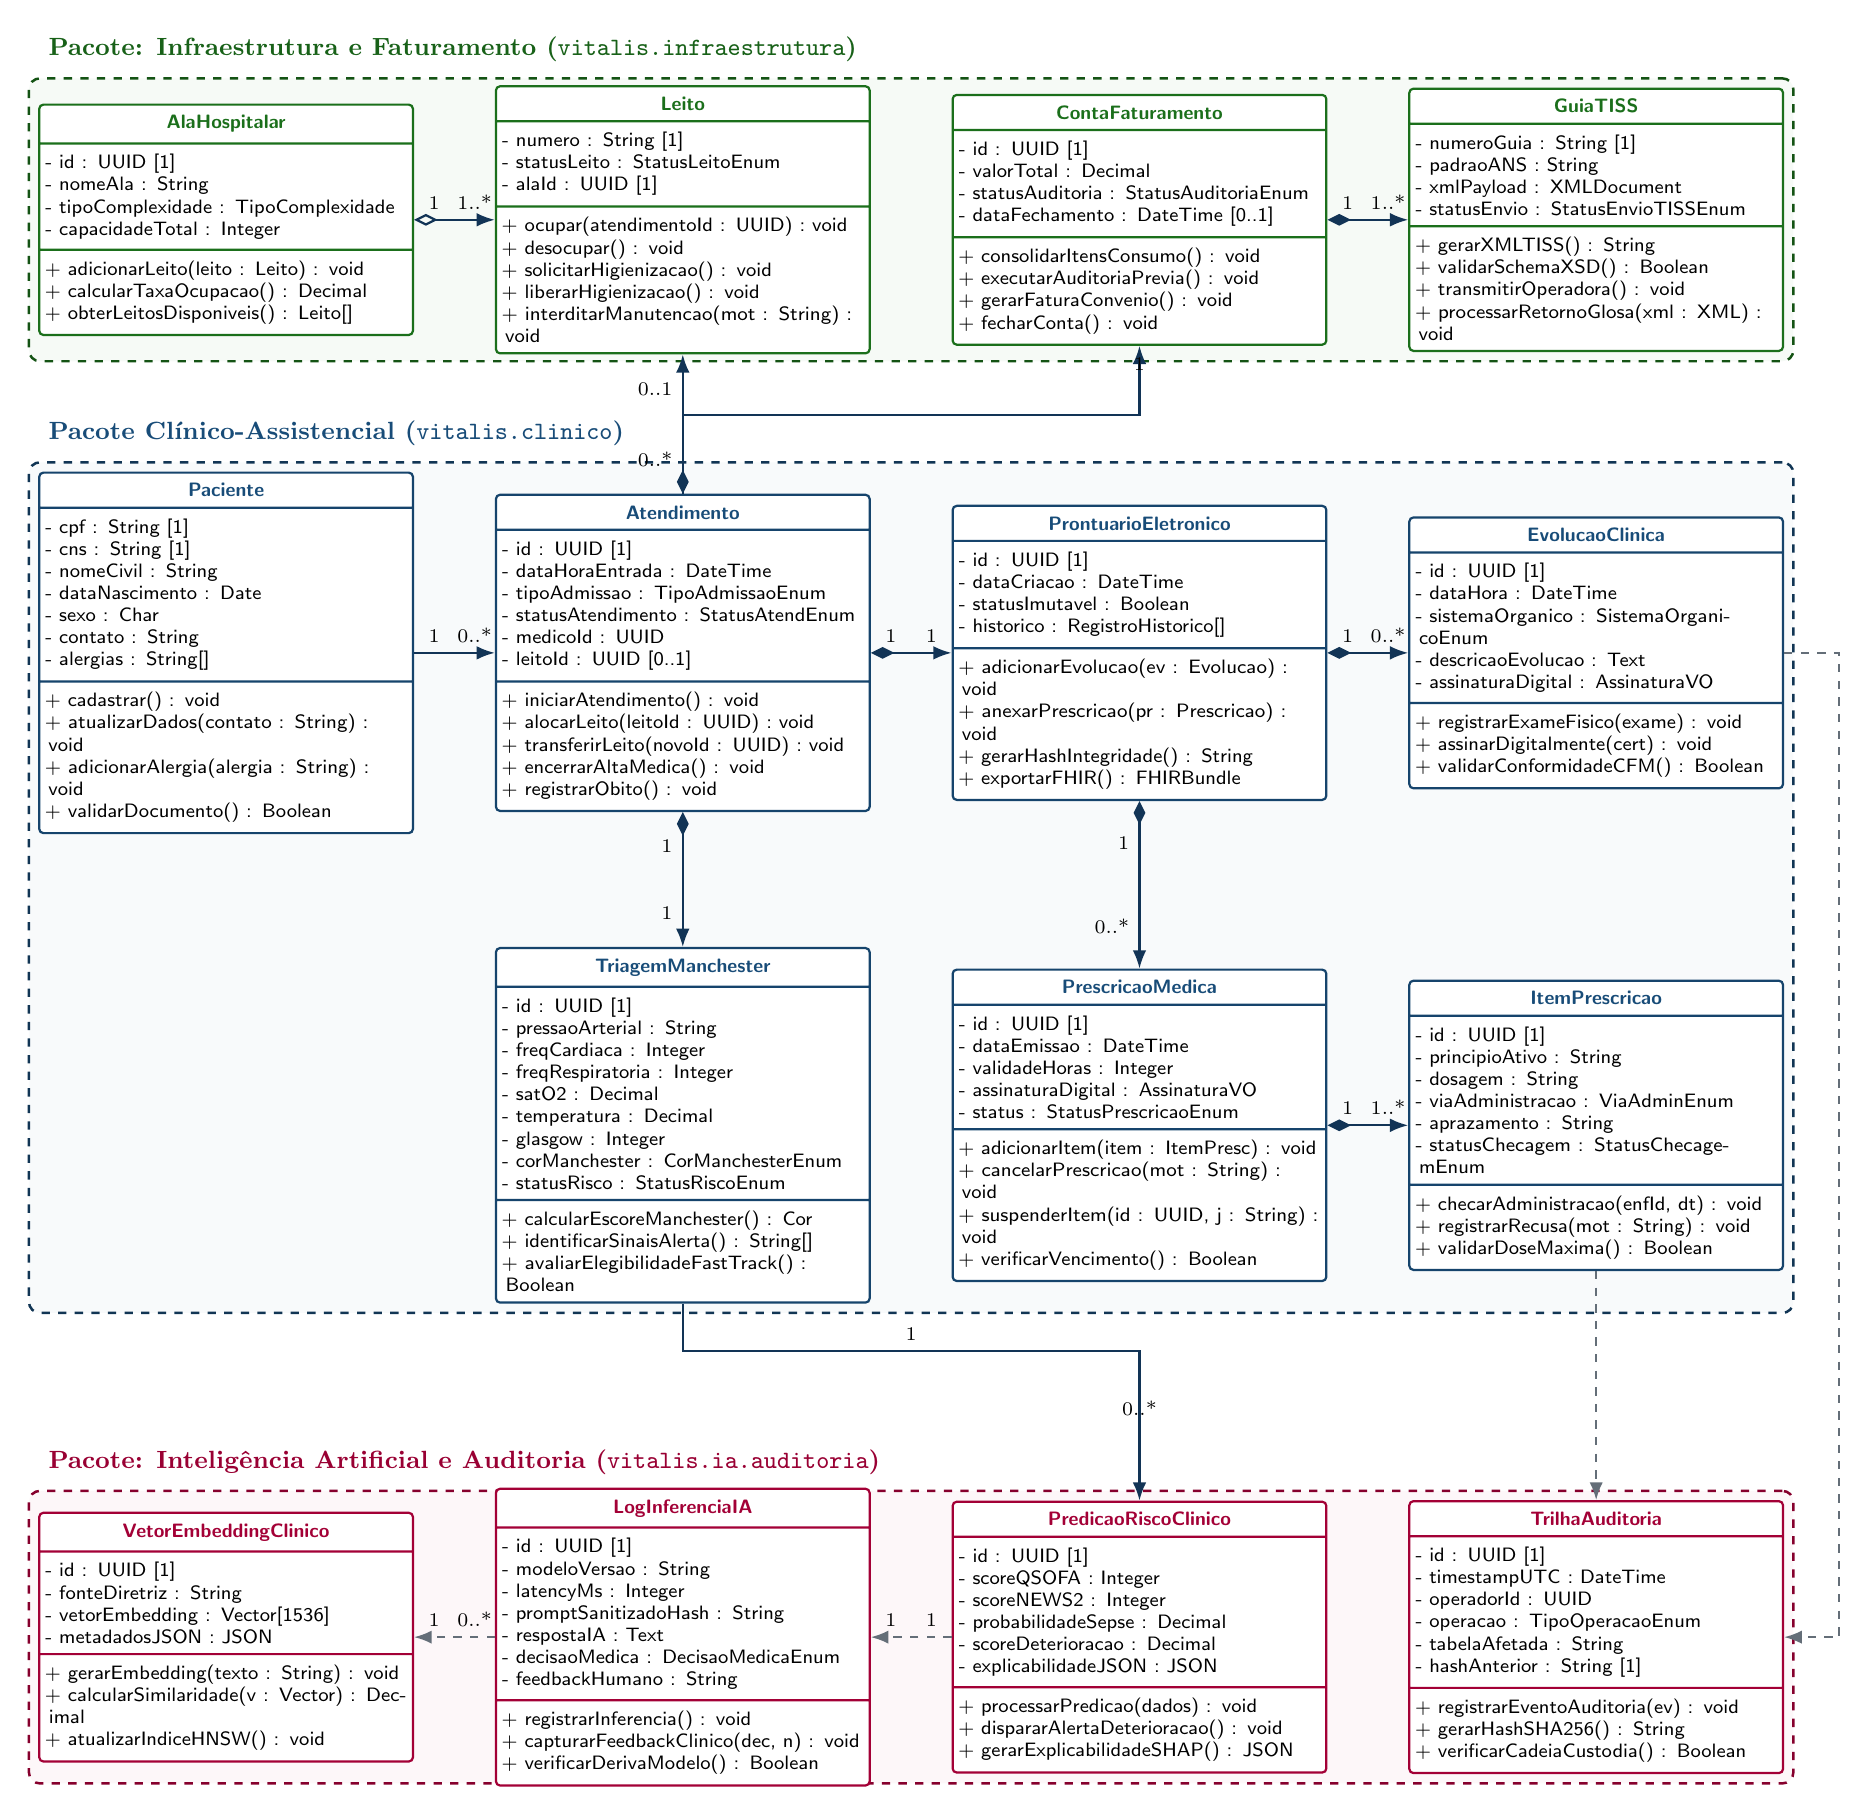
\begin{tikzpicture}[x=1cm, y=1cm, >=Latex]

% --- DEFINICAO DE ESTILOS LOCAIS DE CLASSES UML ---
\tikzset{
  umlClassClinico/.style={
    draw=vitalisblue!90!black,
    fill=white,
    rectangle split,
    rectangle split parts=3,
    rectangle split draw splits=true,
    rounded corners=1.5pt,
    text width=4.5cm,
    font=\scriptsize\sffamily,
    align=left,
    inner sep=3.5pt,
    line width=0.8pt
  },
  umlClassInfra/.style={
    draw=vitalisgreen!80!black,
    fill=white,
    rectangle split,
    rectangle split parts=3,
    rectangle split draw splits=true,
    rounded corners=1.5pt,
    text width=4.5cm,
    font=\scriptsize\sffamily,
    align=left,
    inner sep=3.5pt,
    line width=0.8pt
  },
  umlClassIA/.style={
    draw=purple!85!black,
    fill=white,
    rectangle split,
    rectangle split parts=3,
    rectangle split draw splits=true,
    rounded corners=1.5pt,
    text width=4.5cm,
    font=\scriptsize\sffamily,
    align=left,
    inner sep=3.5pt,
    line width=0.8pt
  },
  umlComposition/.style={
    {Diamond[fill=vitalisdark, length=3.0mm]}-Latex,
    draw=vitalisdark,
    line width=0.8pt
  },
  umlAggregation/.style={
    {Diamond[open, length=3.0mm]}-Latex,
    draw=vitalisdark,
    line width=0.8pt
  },
  umlAssociation/.style={
    -Latex,
    draw=vitalisdark,
    line width=0.8pt
  },
  umlDependency/.style={
    -Latex,
    dashed,
    draw=vitalisgray,
    line width=0.75pt
  }
}

% ==============================================================================
% LINHA 1: PACOTE DE INFRAESTRUTURA E FATURAMENTO (Y = 14.5)
% ==============================================================================
\node[umlClassInfra] at (0, 14.5) (AlaHospitalar) {
  \textbf{\centerline{\textcolor{vitalisgreen!80!black}{AlaHospitalar}}}
  \nodepart{second}
  - id : UUID [1] \\
  - nomeAla : String \\
  - tipoComplexidade : TipoComplexidade \\
  - capacidadeTotal : Integer
  \nodepart{third}
  + adicionarLeito(leito : Leito) : void \\
  + calcularTaxaOcupacao() : Decimal \\
  + obterLeitosDisponiveis() : Leito[]
};

\node[umlClassInfra] at (5.8, 14.5) (Leito) {
  \textbf{\centerline{\textcolor{vitalisgreen!80!black}{Leito}}}
  \nodepart{second}
  - numero : String [1] \\
  - statusLeito : StatusLeitoEnum \\
  - alaId : UUID [1]
  \nodepart{third}
  + ocupar(atendimentoId : UUID) : void \\
  + desocupar() : void \\
  + solicitarHigienizacao() : void \\
  + liberarHigienizacao() : void \\
  + interditarManutencao(mot : String) : void
};

\node[umlClassInfra] at (11.6, 14.5) (ContaFaturamento) {
  \textbf{\centerline{\textcolor{vitalisgreen!80!black}{ContaFaturamento}}}
  \nodepart{second}
  - id : UUID [1] \\
  - valorTotal : Decimal \\
  - statusAuditoria : StatusAuditoriaEnum \\
  - dataFechamento : DateTime [0..1]
  \nodepart{third}
  + consolidarItensConsumo() : void \\
  + executarAuditoriaPrevia() : void \\
  + gerarFaturaConvenio() : void \\
  + fecharConta() : void
};

\node[umlClassInfra] at (17.4, 14.5) (GuiaTISS) {
  \textbf{\centerline{\textcolor{vitalisgreen!80!black}{GuiaTISS}}}
  \nodepart{second}
  - numeroGuia : String [1] \\
  - padraoANS : String \\
  - xmlPayload : XMLDocument \\
  - statusEnvio : StatusEnvioTISSEnum
  \nodepart{third}
  + gerarXMLTISS() : String \\
  + validarSchemaXSD() : Boolean \\
  + transmitirOperadora() : void \\
  + processarRetornoGlosa(xml : XML) : void
};

% ==============================================================================
% PACOTE CLINICO-ASSISTENCIAL: LINHA SUPERIOR (Y = 9.0)
% ==============================================================================
\node[umlClassClinico] at (0, 9.0) (Paciente) {
  \textbf{\centerline{\textcolor{vitalisblue}{Paciente}}}
  \nodepart{second}
  - cpf : String [1] \\
  - cns : String [1] \\
  - nomeCivil : String \\
  - dataNascimento : Date \\
  - sexo : Char \\
  - contato : String \\
  - alergias : String[]
  \nodepart{third}
  + cadastrar() : void \\
  + atualizarDados(contato : String) : void \\
  + adicionarAlergia(alergia : String) : void \\
  + validarDocumento() : Boolean
};

\node[umlClassClinico] at (5.8, 9.0) (Atendimento) {
  \textbf{\centerline{\textcolor{vitalisblue}{Atendimento}}}
  \nodepart{second}
  - id : UUID [1] \\
  - dataHoraEntrada : DateTime \\
  - tipoAdmissao : TipoAdmissaoEnum \\
  - statusAtendimento : StatusAtendEnum \\
  - medicoId : UUID \\
  - leitoId : UUID [0..1]
  \nodepart{third}
  + iniciarAtendimento() : void \\
  + alocarLeito(leitoId : UUID) : void \\
  + transferirLeito(novoId : UUID) : void \\
  + encerrarAltaMedica() : void \\
  + registrarObito() : void
};

\node[umlClassClinico] at (11.6, 9.0) (ProntuarioEletronico) {
  \textbf{\centerline{\textcolor{vitalisblue}{ProntuarioEletronico}}}
  \nodepart{second}
  - id : UUID [1] \\
  - dataCriacao : DateTime \\
  - statusImutavel : Boolean \\
  - historico : RegistroHistorico[]
  \nodepart{third}
  + adicionarEvolucao(ev : Evolucao) : void \\
  + anexarPrescricao(pr : Prescricao) : void \\
  + gerarHashIntegridade() : String \\
  + exportarFHIR() : FHIRBundle
};

\node[umlClassClinico] at (17.4, 9.0) (EvolucaoClinica) {
  \textbf{\centerline{\textcolor{vitalisblue}{EvolucaoClinica}}}
  \nodepart{second}
  - id : UUID [1] \\
  - dataHora : DateTime \\
  - sistemaOrganico : SistemaOrganicoEnum \\
  - descricaoEvolucao : Text \\
  - assinaturaDigital : AssinaturaVO
  \nodepart{third}
  + registrarExameFisico(exame) : void \\
  + assinarDigitalmente(cert) : void \\
  + validarConformidadeCFM() : Boolean
};

% ==============================================================================
% PACOTE CLINICO-ASSISTENCIAL: LINHA INFERIOR (Y = 3.0)
% ==============================================================================
\node[umlClassClinico] at (5.8, 3.0) (TriagemManchester) {
  \textbf{\centerline{\textcolor{vitalisblue}{TriagemManchester}}}
  \nodepart{second}
  - id : UUID [1] \\
  - pressaoArterial : String \\
  - freqCardiaca : Integer \\
  - freqRespiratoria : Integer \\
  - satO2 : Decimal \\
  - temperatura : Decimal \\
  - glasgow : Integer \\
  - corManchester : CorManchesterEnum \\
  - statusRisco : StatusRiscoEnum
  \nodepart{third}
  + calcularEscoreManchester() : Cor \\
  + identificarSinaisAlerta() : String[] \\
  + avaliarElegibilidadeFastTrack() : Boolean
};

\node[umlClassClinico] at (11.6, 3.0) (PrescricaoMedica) {
  \textbf{\centerline{\textcolor{vitalisblue}{PrescricaoMedica}}}
  \nodepart{second}
  - id : UUID [1] \\
  - dataEmissao : DateTime \\
  - validadeHoras : Integer \\
  - assinaturaDigital : AssinaturaVO \\
  - status : StatusPrescricaoEnum
  \nodepart{third}
  + adicionarItem(item : ItemPresc) : void \\
  + cancelarPrescricao(mot : String) : void \\
  + suspenderItem(id : UUID, j : String) : void \\
  + verificarVencimento() : Boolean
};

\node[umlClassClinico] at (17.4, 3.0) (ItemPrescricao) {
  \textbf{\centerline{\textcolor{vitalisblue}{ItemPrescricao}}}
  \nodepart{second}
  - id : UUID [1] \\
  - principioAtivo : String \\
  - dosagem : String \\
  - viaAdministracao : ViaAdminEnum \\
  - aprazamento : String \\
  - statusChecagem : StatusChecagemEnum
  \nodepart{third}
  + checarAdministracao(enfId, dt) : void \\
  + registrarRecusa(mot : String) : void \\
  + validarDoseMaxima() : Boolean
};

% ==============================================================================
% LINHA 4: PACOTE DE INTELIGENCIA ARTIFICIAL E AUDITORIA (Y = -3.5)
% ==============================================================================
\node[umlClassIA] at (0, -3.5) (VetorEmbeddingClinico) {
  \textbf{\centerline{\textcolor{purple!85!black}{VetorEmbeddingClinico}}}
  \nodepart{second}
  - id : UUID [1] \\
  - fonteDiretriz : String \\
  - vetorEmbedding : Vector[1536] \\
  - metadadosJSON : JSON
  \nodepart{third}
  + gerarEmbedding(texto : String) : void \\
  + calcularSimilaridade(v : Vector) : Decimal \\
  + atualizarIndiceHNSW() : void
};

\node[umlClassIA] at (5.8, -3.5) (LogInferenciaIA) {
  \textbf{\centerline{\textcolor{purple!85!black}{LogInferenciaIA}}}
  \nodepart{second}
  - id : UUID [1] \\
  - modeloVersao : String \\
  - latencyMs : Integer \\
  - promptSanitizadoHash : String \\
  - respostaIA : Text \\
  - decisaoMedica : DecisaoMedicaEnum \\
  - feedbackHumano : String
  \nodepart{third}
  + registrarInferencia() : void \\
  + capturarFeedbackClinico(dec, n) : void \\
  + verificarDerivaModelo() : Boolean
};

\node[umlClassIA] at (11.6, -3.5) (PredicaoRiscoClinico) {
  \textbf{\centerline{\textcolor{purple!85!black}{PredicaoRiscoClinico}}}
  \nodepart{second}
  - id : UUID [1] \\
  - scoreQSOFA : Integer \\
  - scoreNEWS2 : Integer \\
  - probabilidadeSepse : Decimal \\
  - scoreDeterioracao : Decimal \\
  - explicabilidadeJSON : JSON
  \nodepart{third}
  + processarPredicao(dados) : void \\
  + dispararAlertaDeterioracao() : void \\
  + gerarExplicabilidadeSHAP() : JSON
};

\node[umlClassIA] at (17.4, -3.5) (TrilhaAuditoria) {
  \textbf{\centerline{\textcolor{purple!85!black}{TrilhaAuditoria}}}
  \nodepart{second}
  - id : UUID [1] \\
  - timestampUTC : DateTime \\
  - operadorId : UUID \\
  - operacao : TipoOperacaoEnum \\
  - tabelaAfetada : String \\
  - hashAnterior : String [1]
  \nodepart{third}
  + registrarEventoAuditoria(ev) : void \\
  + gerarHashSHA256() : String \\
  + verificarCadeiaCustodia() : Boolean
};

% ==============================================================================
% CAIXAS DE PACOTE (BACKGROUND LAYER)
% ==============================================================================
\begin{scope}[on background layer]
  % Pacote Infraestrutura
  \node[draw=vitalisgreen!60!black, fill=vitalisgreen!4, rounded corners=4pt, line width=0.9pt, dashed,
        fit=(AlaHospitalar) (GuiaTISS)] (boxInfra) {};
  \node[anchor=south west, font=\small\bfseries\color{vitalisgreen!70!black}, xshift=4pt, yshift=2pt] 
        at (boxInfra.north west) {Pacote: Infraestrutura e Faturamento (\texttt{vitalis.infraestrutura})};

  % Pacote Clinico
  \node[draw=vitalisblue!70!black, fill=vitalisblue!3, rounded corners=4pt, line width=0.9pt, dashed,
        fit=(Paciente) (EvolucaoClinica) (TriagemManchester) (ItemPrescricao)] (boxClinico) {};
  \node[anchor=south west, font=\small\bfseries\color{vitalisblue}, xshift=4pt, yshift=2pt] 
        at (boxClinico.north west) {Pacote Clínico-Assistencial (\texttt{vitalis.clinico})};

  % Pacote IA e Auditoria
  \node[draw=purple!70!black, fill=purple!3, rounded corners=4pt, line width=0.9pt, dashed,
        fit=(VetorEmbeddingClinico) (TrilhaAuditoria)] (boxIA) {};
  \node[anchor=south west, font=\small\bfseries\color{purple!80!black}, xshift=4pt, yshift=2pt] 
        at (boxIA.north west) {Pacote: Inteligência Artificial e Auditoria (\texttt{vitalis.ia.auditoria})};
\end{scope}

% ==============================================================================
% CONEXOES E RELACIONAMENTOS ARQUITETURAIS
% ==============================================================================

% 1. AlaHospitalar agrega Leito (1 para 1..*)
\draw[umlAggregation] (AlaHospitalar) -- node[above, near start]{\scriptsize 1} node[above, near end]{\scriptsize 1..*} (Leito);

% 2. ContaFaturamento compõe GuiaTISS (1 para 1..*)
\draw[umlComposition] (ContaFaturamento) -- node[above, near start]{\scriptsize 1} node[above, near end]{\scriptsize 1..*} (GuiaTISS);

% 3. Paciente associado a Atendimento (1 para 0..*)
\draw[umlAssociation] (Paciente) -- node[above, near start]{\scriptsize 1} node[above, near end]{\scriptsize 0..*} (Atendimento);

% 4. Atendimento e Leito (0..* para 0..1)
\draw[umlAssociation] (Atendimento) -- node[left, near start]{\scriptsize 0..*} node[left, near end]{\scriptsize 0..1} (Leito);

% 5. Atendimento compõe ContaFaturamento (1 para 1)
\draw[umlComposition] (Atendimento.north) -- ++(0,1.0) -| node[above, near end]{\scriptsize 1} (ContaFaturamento.south);

% 6. Atendimento compõe TriagemManchester (1 para 1)
\draw[umlComposition] (Atendimento) -- node[left, near start]{\scriptsize 1} node[left, near end]{\scriptsize 1} (TriagemManchester);

% 7. Atendimento compõe ProntuarioEletronico (1 para 1)
\draw[umlComposition] (Atendimento) -- node[above, near start]{\scriptsize 1} node[above, near end]{\scriptsize 1} (ProntuarioEletronico);

% 8. ProntuarioEletronico compõe EvolucaoClinica (1 para 0..*)
\draw[umlComposition] (ProntuarioEletronico) -- node[above, near start]{\scriptsize 1} node[above, near end]{\scriptsize 0..*} (EvolucaoClinica);

% 9. ProntuarioEletronico compõe PrescricaoMedica (1 para 0..*)
\draw[umlComposition] (ProntuarioEletronico) -- node[left, near start]{\scriptsize 1} node[left, near end]{\scriptsize 0..*} (PrescricaoMedica);

% 10. PrescricaoMedica compõe ItemPrescricao (1 para 1..*)
\draw[umlComposition] (PrescricaoMedica) -- node[above, near start]{\scriptsize 1} node[above, near end]{\scriptsize 1..*} (ItemPrescricao);

% 11. TriagemManchester gera PredicaoRiscoClinico (1 para 0..*)
\draw[umlAssociation] (TriagemManchester.south) -- ++(0,-0.6) -| node[above, near start]{\scriptsize 1} node[above, near end]{\scriptsize 0..*} (PredicaoRiscoClinico.north);

% 12. PredicaoRiscoClinico depende de LogInferenciaIA (1 para 1)
\draw[umlDependency] (PredicaoRiscoClinico) -- node[above, near start]{\scriptsize 1} node[above, near end]{\scriptsize 1} (LogInferenciaIA);

% 13. LogInferenciaIA consulta VetorEmbeddingClinico (0..* para 1)
\draw[umlDependency] (LogInferenciaIA) -- node[above, near start]{\scriptsize 0..*} node[above, near end]{\scriptsize 1} (VetorEmbeddingClinico);

% 14. TrilhaAuditoria intercepta registros sensíveis
\draw[umlDependency] (ItemPrescricao.south) -- (TrilhaAuditoria.north);
\draw[umlDependency] (EvolucaoClinica.east) -- ++(0.7,0) |- (TrilhaAuditoria.east);

\end{tikzpicture}
}
\caption{Diagrama Estrutural de Classes UML do Sistema Vitalis v2.0}
\label{fig:diagrama_classes_geral}
\end{figure}

% ==============================================================================
% 8.3 ANALISE DETALHADA DAS CLASSES DO DOMINIO CLINICO-ASSISTENCIAL
% ==============================================================================
\subsection{Detalhamento do Pacote Clínico-Assistencial}
\label{subsec:detalhe_clinico}

O pacote clínico concentra os registros de saúde gerados durante a passagem do paciente pela instituição. As classes que o integram foram desenhadas segundo as normas de guarda e autenticidade do Conselho Federal de Medicina (CFM) \cite{cfm_prontuario:2007, cfm_digital:2021} e as recomendações internacionais de interoperabilidade do padrão HL7 FHIR Release 4 \cite{hl7_fhir:2019}.

\subsubsection{Classe Paciente}
A classe \texttt{Paciente} mantém os dados cadastrais primários e os antecedentes imunoalérgicos do indivíduo. A integridade cadastral é aferida mediante validação dos dígitos verificadores do CPF e do identificador unificado do Cartão Nacional de Saúde (CNS). Para mitigar riscos iatrogênicos em prescrições, a coleção \texttt{alergias} armazena princípios ativos e alérgenos declarados.

\begingroup
\small
\noindent\begin{tabularx}{\linewidth}{l >{\raggedright\arraybackslash}p{5.7cm} >{\raggedright\arraybackslash}X}
\toprule
\textbf{Elemento} & \textbf{Assinatura / Tipo} & \textbf{Descrição Técnica e Regra de Negócio} \\
\midrule
Atributo & \texttt{- cpf : String [1]} & Chave natural de 11 dígitos; validada na base da Receita Federal. \\
Atributo & \texttt{- cns : String [1]} & Identificador do Cartão Nacional de Saúde (15 dígitos). \\
Atributo & \texttt{- nomeCivil : String} & Nome oficial de registro civil do paciente. \\
Atributo & \texttt{- dataNascimento : Date} & Utilizada no cálculo dinâmico da idade para escores clínicos. \\
Atributo & \texttt{- sexo : Char} & Sexo biológico ('M', 'F', 'I') para parametrização laboratorial. \\
Atributo & \texttt{- contato : String} & Telefone, e-mail e dados de contato do responsável de emergência. \\
Atributo & \texttt{- alergias : String[*]} & Coleção de substâncias e fármacos contraindicados. \\
\midrule
Método & \texttt{+ cadastrar() : void} & Efetua a persistência inicial no banco relacional via repositório. \\
Método & \texttt{+ atualizarDados(c : String) : void} & Altera dados de contato com registro obrigatório de auditoria. \\
Método & \texttt{+ adicionarAlergia(a : String) : void} & Inclui novo alérgeno com validação de unicidade na lista. \\
Método & \texttt{+ validarDocumento() : Boolean} & Executa algoritmo de módulo 11 para verificação do CPF e CNS. \\
\bottomrule
\end{tabularx}
\endgroup

\subsubsection{Classe Atendimento}
A classe \texttt{Atendimento} materializa a estadia do paciente na unidade hospitalar, servindo como ponto focal de agregação para triagens, prontuários, alocações de leito e faturamento. Seu ciclo de vida obedece à máquina de estados descrita no requisito RF-002, transitando entre \texttt{AguardandoTriagem}, \texttt{EmTriagem}, \texttt{AguardandoConsulta}, \texttt{EmAtendimento}, \texttt{Internado}, \texttt{AltaMedica}, \texttt{Transferido} e \texttt{Obito}.

\begingroup
\small
\noindent\begin{tabularx}{\linewidth}{l >{\raggedright\arraybackslash}p{5.7cm} >{\raggedright\arraybackslash}X}
\toprule
\textbf{Elemento} & \textbf{Assinatura / Tipo} & \textbf{Descrição Técnica e Regra de Negócio} \\
\midrule
Atributo & \texttt{- id : UUID [1]} & Chave substituta universalmente única (RFC 4122). \\
Atributo & \texttt{- dataHoraEntrada : DateTime} & Carimbo de data/hora (UTC) do acolhimento na recepção. \\
Atributo & \texttt{- tipoAdmissao : TipoAdmissao} & Enumerador: \texttt{Eletivo}, \texttt{Urgencia}, \texttt{Emergencia}. \\
Atributo & \texttt{- statusAtendimento : Status} & Estado operacional corrente do fluxo assistencial. \\
Atributo & \texttt{- medicoId : UUID} & Identificador do profissional médico responsável pela admissão. \\
Atributo & \texttt{- leitoId : UUID [0..1]} & Referência opcional ao leito ocupado em caso de internação. \\
\midrule
Método & \texttt{+ iniciarAtendimento() : void} & Dispara o início da sessão assistencial e posiciona na fila. \\
Método & \texttt{+ alocarLeito(id : UUID) : void} & Vincula o atendimento a um leito disponível, alterando seu estado. \\
Método & \texttt{+ transferirLeito(novoId : UUID)} & Executa a realocação física com rastreamento de histórico. \\
Método & \texttt{+ encerrarAltaMedica() : void} & Formaliza a alta, liberando o leito para higienização predial. \\
Método & \texttt{+ registrarObito() : void} & Bloqueia novos lançamentos clínicos e encaminha declaração. \\
\bottomrule
\end{tabularx}
\endgroup

\subsubsection{Classe TriagemManchester}
A classe \texttt{TriagemManchester} registra a avaliação de gravidade conduzida pela equipe de enfermagem, parametrizada segundo os descritores do Protocolo de Manchester \cite{manchester:2014}. A aferição reúne cinco sinais vitais quantitativos e o nível de consciência pela Escala de Coma de Glasgow, computando a cor correspondente e o tempo-alvo máximo para o primeiro atendimento médico.

\begingroup
\small
\noindent\begin{tabularx}{\linewidth}{l >{\raggedright\arraybackslash}p{5.7cm} >{\raggedright\arraybackslash}X}
\toprule
\textbf{Elemento} & \textbf{Assinatura / Tipo} & \textbf{Descrição Técnica e Regra de Negócio} \\
\midrule
Atributo & \texttt{- id : UUID [1]} & Identificador primário imutável da triagem. \\
Atributo & \texttt{- pressaoArterial : String} & Pressão arterial sistólica/diastólica em mmHg (ex.: "120/80"). \\
Atributo & \texttt{- freqCardiaca : Integer} & Frequência cardíaca em batimentos por minuto (bpm). \\
Atributo & \texttt{- freqRespiratoria : Integer} & Frequência respiratória em incursões por minuto (irpm). \\
Atributo & \texttt{- satO2 : Decimal} & Saturação periférica de oxigênio em porcentagem (\%). \\
Atributo & \texttt{- temperatura : Decimal} & Temperatura axilar aferida em graus Celsius ($^\circ$C). \\
Atributo & \texttt{- glasgow : Integer} & Pontuação na Escala de Glasgow (valor inteiro entre 3 e 15). \\
Atributo & \texttt{- corManchester : CorEnum} & Vermelho (imediato), Laranja (10 min), Amarelo (60 min), etc. \\
Atributo & \texttt{- statusRisco : StatusRisco} & Classificação auxiliar: \texttt{Estavel}, \texttt{Alerta}, \texttt{Critico}. \\
\midrule
Método & \texttt{+ calcularEscore() : CorEnum} & Aplica a árvore de decisão do protocolo para sugerir prioridade. \\
Método & \texttt{+ identificarSinaisAlerta() : List} & Retorna discriminares clínicos compatíveis com sepse precoce. \\
Método & \texttt{+ avaliarFastTrack() : Boolean} & Avalia elegibilidade para encaminhamento a linhas de cuidado rápido. \\
\bottomrule
\end{tabularx}
\endgroup

\subsubsection{Classe ProntuarioEletronico}
A classe \texttt{ProntuarioEletronico} consolida o histórico médico e as condutas terapêuticas do paciente. Em conformidade com a Resolução CFM nº 1.821/2007 \cite{cfm_prontuario:2007}, os registros vinculados ao prontuário são estritamente cumulativos e imutáveis; correções exigem a adição de novas notas de retificação sem sobrescrita do conteúdo histórico.

\begingroup
\small
\noindent\begin{tabularx}{\linewidth}{l >{\raggedright\arraybackslash}p{5.7cm} >{\raggedright\arraybackslash}X}
\toprule
\textbf{Elemento} & \textbf{Assinatura / Tipo} & \textbf{Descrição Técnica e Regra de Negócio} \\
\midrule
Atributo & \texttt{- id : UUID [1]} & Identificador único global do repositório clínico do paciente. \\
Atributo & \texttt{- dataCriacao : DateTime} & Carimbo de abertura do prontuário eletrônico institucional. \\
Atributo & \texttt{- statusImutavel : Boolean} & Flag de garantia de não-exclusão lógica e física dos dados. \\
Atributo & \texttt{- historico : Registro[]} & Coleção agregada de eventos clínicos indexados cronologicamente. \\
\midrule
Método & \texttt{+ adicionarEvolucao(e) : void} & Anexa uma nova nota médica estruturada ao histórico. \\
Método & \texttt{+ anexarPrescricao(p) : void} & Vincula a prescrição médica digital aprovada ao atendimento. \\
Método & \texttt{+ gerarHashIntegridade() : String} & Computa o resumo criptográfico SHA-256 do encadeamento do prontuário. \\
Método & \texttt{+ exportarFHIR() : FHIRBundle} & Converte o histórico em recursos JSON padronizados HL7 FHIR R4 \cite{hl7_fhir:2019}. \\
\bottomrule
\end{tabularx}
\endgroup

\subsubsection{Classe EvolucaoClinica}
A classe \texttt{EvolucaoClinica} modela a descrição formal das alterações no estado de saúde do paciente, organizada pelo formato SOAP (Subjetivo, Objetivo, Avaliação e Plano) e segregada por sistemas orgânicos (cardiovascular, neurológico, respiratório, entre outros). Toda evolução requer assinatura digital qualificada (padrão ICP-Brasil) conforme a Resolução CFM nº 2.299/2021 \cite{cfm_digital:2021}.

\begingroup
\small
\noindent\begin{tabularx}{\linewidth}{l >{\raggedright\arraybackslash}p{5.7cm} >{\raggedright\arraybackslash}X}
\toprule
\textbf{Elemento} & \textbf{Assinatura / Tipo} & \textbf{Descrição Técnica e Regra de Negócio} \\
\midrule
Atributo & \texttt{- id : UUID [1]} & Identificador primário da nota evolutiva. \\
Atributo & \texttt{- dataHora : DateTime} & Instante exato da realização do exame clínico e redação. \\
Atributo & \texttt{- sistemaOrganico : Sistema} & Sistema biológico em foco (ex.: \texttt{Cardiovascular}, \texttt{Renal}). \\
Atributo & \texttt{- descricaoEvolucao : Text} & Corpo do texto clínico contendo a propedêutica e conduta. \\
Atributo & \texttt{- assinaturaDigital : AssinaturaVO} & Metadados do certificado digital X.509, carimbo do tempo e hash. \\
\midrule
Método & \texttt{+ registrarExameFisico(d) : void} & Registra dados propedêuticos objetivos e achados ectoscópicos. \\
Método & \texttt{+ assinarDigitalmente(c) : void} & Assina o documento via certificado ICP-Brasil, tornando-o imutável. \\
Método & \texttt{+ validarConformidadeCFM() : Bool} & Verifica a presença de CRM ativo, carimbo e assinatura válida. \\
\bottomrule
\end{tabularx}
\endgroup

\subsubsection{Classe PrescricaoMedica}
A classe \texttt{PrescricaoMedica} reúne as ordens de administração farmacológica, fluidoterapia e procedimentos profiláticos emitidos pelo médico responsável. No Vitalis v2.0, as prescrições possuem validade máxima parametrizada de 24 horas (exigindo reavaliação médica diária) e compõem uma relação forte com seus itens.

\begingroup
\small
\noindent\begin{tabularx}{\linewidth}{l >{\raggedright\arraybackslash}p{5.7cm} >{\raggedright\arraybackslash}X}
\toprule
\textbf{Elemento} & \textbf{Assinatura / Tipo} & \textbf{Descrição Técnica e Regra de Negócio} \\
\midrule
Atributo & \texttt{- id : UUID [1]} & Identificador único da folha de prescrição diária. \\
Atributo & \texttt{- dataEmissao : DateTime} & Carimbo de data/hora da emissão médica formal. \\
Atributo & \texttt{- validadeHoras : Integer} & Janela de vigência legal da prescrição (padrão: 24 horas). \\
Atributo & \texttt{- assinaturaDigital : AssinaturaVO} & Assinatura eletrônica do médico prescritor (ICP-Brasil). \\
Atributo & \texttt{- status : StatusPrescricao} & Enumerador: \texttt{Ativa}, \texttt{Vencida}, \texttt{Suspensa}, \texttt{Cancelada}. \\
\midrule
Método & \texttt{+ adicionarItem(i : Item) : void} & Adiciona novo item terapêutico após checagem pelo Copiloto de IA. \\
Método & \texttt{+ cancelarPrescricao(m : String)} & Cancela a prescrição inteira com justificativa clínica compulsória. \\
Método & \texttt{+ suspenderItem(id : UUID, j : String)} & Suspende fármaco individual sem invalidar o restante da folha. \\
Método & \texttt{+ verificarVencimento() : Boolean} & Avalia se o tempo decorrido ultrapassou a janela de 24 horas. \\
\bottomrule
\end{tabularx}
\endgroup

\subsubsection{Classe ItemPrescricao}
A classe \texttt{ItemPrescricao} representa cada linha individual de medicação prescrita, contendo o princípio ativo, posologia, via de administração e horários de aprazamento. Durante o ciclo assistencial, a equipe de enfermagem executa a checagem beira-leito, com validação do paciente e registro de eventuais recusas ou efeitos adversos.

\begingroup
\small
\noindent\begin{tabularx}{\linewidth}{l >{\raggedright\arraybackslash}p{5.7cm} >{\raggedright\arraybackslash}X}
\toprule
\textbf{Elemento} & \textbf{Assinatura / Tipo} & \textbf{Descrição Técnica e Regra de Negócio} \\
\midrule
Atributo & \texttt{- id : UUID [1]} & Identificador unívoco do item farmacológico. \\
Atributo & \texttt{- principioAtivo : String} & Denominação Comum Brasileira (DCB) do medicamento. \\
Atributo & \texttt{- dosagem : String} & Concentração e quantidade prescrita (ex.: "500 mg", "10 ml"). \\
Atributo & \texttt{- viaAdministracao : ViaEnum} & Via de aplicação: \texttt{Oral}, \texttt{Intravenosa}, \texttt{Inalatoria}, etc. \\
Atributo & \texttt{- aprazamento : String} & Escala temporal de administração (ex.: "6/6h", "dose unica"). \\
Atributo & \texttt{- statusChecagem : StatusChec} & Enumerador: \texttt{Pendente}, \texttt{Checado}, \texttt{Recusado}. \\
\midrule
Método & \texttt{+ checarAdministracao(enfId, dt)} & Registra a efetiva infusão beira-leito com biometria ou crachá. \\
Método & \texttt{+ registrarRecusa(m : String)} & Registra a recusa fundamentada do paciente ou intercorrência. \\
Método & \texttt{+ validarDoseMaxima() : Boolean} & Verifica se a dose diária acumulada respeita os limites da bula. \\
\bottomrule
\end{tabularx}
\endgroup

% ==============================================================================
% 8.4 ANALISE DETALHADA DE INFRAESTRUTURA E FATURAMENTO
% ==============================================================================
\subsection{Detalhamento do Pacote de Infraestrutura e Faturamento}
\label{subsec:detalhe_infra_faturamento}

A eficiência econômica e operacional do hospital depende da sincronia precisa entre a infraestrutura de internação e os processos de faturamento para as operadoras de planos de saúde e Sistema Único de Saúde.

\subsubsection{Classe AlaHospitalar}
A classe \texttt{AlaHospitalar} delimita uma divisão física e funcional da instituição, categorizada por complexidade assistencial (enfermaria clínica, UTI adulto, UTI neonatal, unidade cirúrgica). Ela congrega os leitos físicos por meio de agregação e provê métodos para cálculo dinâmico da taxa de ocupação.

\begingroup
\small
\noindent\begin{tabularx}{\linewidth}{l >{\raggedright\arraybackslash}p{5.7cm} >{\raggedright\arraybackslash}X}
\toprule
\textbf{Elemento} & \textbf{Assinatura / Tipo} & \textbf{Descrição Técnica e Regra de Negócio} \\
\midrule
Atributo & \texttt{- id : UUID [1]} & Chave primária da unidade física ou setor hospitalar. \\
Atributo & \texttt{- nomeAla : String} & Descrição institucional (ex.: "UTI Coronariana - Bloco B"). \\
Atributo & \texttt{- tipoComplexidade : TipoEnum} & Nível de assistência: \texttt{Baixa}, \texttt{Media}, \texttt{UTI\_Adulto}, etc. \\
Atributo & \texttt{- capacidadeTotal : Integer} & Quantidade máxima de leitos estruturados na ala. \\
\midrule
Método & \texttt{+ adicionarLeito(l : Leito) : void} & Associa um novo leito físico mantendo a restrição de capacidade. \\
Método & \texttt{+ calcularTaxaOcupacao() : Decimal} & Retorna a razão percentual entre leitos ocupados e o total ativo. \\
Método & \texttt{+ obterLeitosDisponiveis() : List} & Consulta leitos com estado operacional estritamente \texttt{Livre}. \\
\bottomrule
\end{tabularx}
\endgroup

\subsubsection{Classe Leito}
A classe \texttt{Leito} gerencia o estado operacional do mobiliário e espaço de internação. Para prevenir riscos de infecção hospitalar cruzada e assegurar rotatividade segura, o leito percorre um ciclo obrigatório de higienização antes de ser disponibilizado para novas internações.

\begingroup
\small
\noindent\begin{tabularx}{\linewidth}{l >{\raggedright\arraybackslash}p{5.7cm} >{\raggedright\arraybackslash}X}
\toprule
\textbf{Elemento} & \textbf{Assinatura / Tipo} & \textbf{Descrição Técnica e Regra de Negócio} \\
\midrule
Atributo & \texttt{- numero : String [1]} & Código de identificação visível do leito (ex.: "LEI-204-A"). \\
Atributo & \texttt{- statusLeito : StatusLeitoEnum} & Estados: \texttt{Livre}, \texttt{Ocupado}, \texttt{Higienizacao}, \texttt{Manutencao}. \\
Atributo & \texttt{- alaId : UUID [1]} & Chave estrangeira que referencia a \texttt{AlaHospitalar} de alocação. \\
\midrule
Método & \texttt{+ ocupar(atendId : UUID) : void} & Transiciona o estado para \texttt{Ocupado} e bloqueia novas reservas. \\
Método & \texttt{+ desocupar() : void} & Chaveia para \texttt{Higienizacao} imediatamente após a alta. \\
Método & \texttt{+ solicitarHigienizacao() : void} & Dispara chamado à governança com nível de desinfecção específico. \\
Método & \texttt{+ liberarHigienizacao() : void} & Atualiza para \texttt{Livre} após validação pelo supervisor predial. \\
Método & \texttt{+ interditarManutencao(m : String)} & Bloqueia o leito por avaria mecânica ou manutenção de gases. \\
\bottomrule
\end{tabularx}
\endgroup

\subsubsection{Classe ContaFaturamento}
A classe \texttt{ContaFaturamento} apura os custos diretos da assistência prestada durante o atendimento. Ela consolida diárias de internação, materiais descartáveis, medicamentos administrados e honorários profissionais, executando rotinas automáticas de pré-auditoria para identificar inconsistências cadastrais antes da emissão definitiva da fatura.

\begingroup
\small
\noindent\begin{tabularx}{\linewidth}{l >{\raggedright\arraybackslash}p{5.7cm} >{\raggedright\arraybackslash}X}
\toprule
\textbf{Elemento} & \textbf{Assinatura / Tipo} & \textbf{Descrição Técnica e Regra de Negócio} \\
\midrule
Atributo & \texttt{- id : UUID [1]} & Chave primária da conta médica do atendimento. \\
Atributo & \texttt{- valorTotal : Decimal} & Montante financeiro apurado com precisão monetária (2 casas). \\
Atributo & \texttt{- statusAuditoria : StatusAudit} & Estados: \texttt{EmAberto}, \texttt{PreAuditada}, \texttt{Aprovada}, \texttt{Discrepante}. \\
Atributo & \texttt{- dataFechamento : DateTime [0..1]} & Instante do fechamento administrativo da conta. \\
\midrule
Método & \texttt{+ consolidarItensConsumo() : void} & Cruza itens checados na prescrição com tabela de preços TUSS. \\
Método & \texttt{+ executarAuditoriaPrevia() : void} & Varre a conta em busca de incompatibilidades diagnósticas (CID x TUSS). \\
Método & \texttt{+ gerarFaturaConvenio() : void} & Estrutura a fatura comercial nos padrões do convênio pagador. \\
Método & \texttt{+ fecharConta() : void} & Trava a conta contra novas alterações e autoriza o envio. \\
\bottomrule
\end{tabularx}
\endgroup

\subsubsection{Classe GuiaTISS}
A classe \texttt{GuiaTISS} gera e valida os arquivos XML exigidos pelo padrão de Troca de Informação em Saúde Suplementar (TISS v4.01) da Agência Nacional de Saúde Suplementar (ANS) \cite{ans_tiss:2023}. A classe encapsula a validação estrutural contra esquemas XSD oficiais, realiza a transmissão via barramento SOAP seguro e processa os retornos eletrônicos com mapeamento de eventuais glosas.

\begingroup
\small
\noindent\begin{tabularx}{\linewidth}{l >{\raggedright\arraybackslash}p{5.7cm} >{\raggedright\arraybackslash}X}
\toprule
\textbf{Elemento} & \textbf{Assinatura / Tipo} & \textbf{Descrição Técnica e Regra de Negócio} \\
\midrule
Atributo & \texttt{- numeroGuia : String [1]} & Número único da guia de internação ou consulta (padrão ANS). \\
Atributo & \texttt{- padraoANS : String} & Versão do componente organizacional da ANS (ex.: "v4.01.00"). \\
Atributo & \texttt{- xmlPayload : XMLDocument} & Mensagem estruturada em conformidade com o XSD da ANS. \\
Atributo & \texttt{- statusEnvio : StatusEnvio} & Enumerador: \texttt{Pendente}, \texttt{Transmitida}, \texttt{Aceita}, \texttt{Glosada}. \\
\midrule
Método & \texttt{+ gerarXMLTISS() : String} & Serializa os dados da conta hospitalar na sintaxe XML do padrão TISS. \\
Método & \texttt{+ validarSchemaXSD() : Boolean} & Valida o documento contra a árvore de esquemas XSD da operadora. \\
Método & \texttt{+ transmitirOperadora() : void} & Dispara requisição HTTPS mTLS para o webservice da fonte pagadora. \\
Método & \texttt{+ processarRetornoGlosa(xml) : void} & Extrai códigos de glosa e atualiza a conta para contestação recursal. \\
\bottomrule
\end{tabularx}
\endgroup

% ==============================================================================
% 8.5 ANALISE DETALHADA DO MODULO DE IA E AUDITORIA
% ==============================================================================
\subsection{Detalhamento do Pacote de Inteligência Artificial e Auditoria}
\label{subsec:detalhe_ia_auditoria}

O subsistema de inteligência artificial do Vitalis v2.0 atua exclusivamente como ferramenta consultiva de suporte à decisão clínica, operando sob supervisão médica humana estrita (\textit{human-in-the-loop}).

\subsubsection{Classe PredicaoRiscoClinico}
A classe \texttt{PredicaoRiscoClinico} armazena os resultados inferenciais dos algoritmos de alerta precoce e probabilidade de sepse precoce \cite{singer_sepsis:2016}. Os cálculos baseiam-se em sinais vitais objetivos e contam com matriz de interpretabilidade em formato JSON com valores SHAP \cite{lundberg_shap:2017}, explicitando ao médico os parâmetros que mais contribuíram para o escore de alerta.

\begingroup
\small
\noindent\begin{tabularx}{\linewidth}{l >{\raggedright\arraybackslash}p{5.7cm} >{\raggedright\arraybackslash}X}
\toprule
\textbf{Elemento} & \textbf{Assinatura / Tipo} & \textbf{Descrição Técnica e Regra de Negócio} \\
\midrule
Atributo & \texttt{- id : UUID [1]} & Identificador primário da rodada preditiva. \\
Atributo & \texttt{- scoreQSOFA : Integer} & Pontuação qSOFA (0 a 3) para triagem rápida de sepse à beira-leito. \\
Atributo & \texttt{- scoreNEWS2 : Integer} & Pontuação agregada do National Early Warning Score 2 (0 a 20) \cite{rcp_news2:2017}. \\
Atributo & \texttt{- probabilidadeSepse : Decimal} & Estimativa probabilística calculada por modelo calibrado ($0,00$ a $1,00$). \\
Atributo & \texttt{- scoreDeterioracao : Decimal} & Índice percentual composto de deterioração clínica rápida. \\
Atributo & \texttt{- explicabilidadeJSON : JSON} & Pesos relativos de cada sinal vital derivados via SHAP \cite{lundberg_shap:2017}. \\
\midrule
Método & \texttt{+ processarPredicao(d) : void} & Alimenta os dados de entrada na estratégia algorítmica selecionada. \\
Método & \texttt{+ dispararAlertaDeterioracao()} & Emite evento WebSocket prioritário caso os limiares críticos estourem. \\
Método & \texttt{+ gerarExplicabilidadeSHAP() : JSON} & Computa as contribuições marginais dos sinais para a interface médica. \\
\bottomrule
\end{tabularx}
\endgroup

\subsubsection{Classe LogInferenciaIA}
A classe \texttt{LogInferenciaIA} garante a rastreabilidade total de cada chamada aos modelos preditivos e generativos. Ela registra o hash SHA-256 dos dados sanitizados enviados, a versão exata do modelo, a latência de execução (ms), a sugestão fornecida pela máquina e a decisão clínica tomada pelo profissional de saúde (aceitação integral, modificação da conduta ou rejeição justificada).

\begingroup
\small
\noindent\begin{tabularx}{\linewidth}{l >{\raggedright\arraybackslash}p{5.7cm} >{\raggedright\arraybackslash}X}
\toprule
\textbf{Elemento} & \textbf{Assinatura / Tipo} & \textbf{Descrição Técnica e Regra de Negócio} \\
\midrule
Atributo & \texttt{- id : UUID [1]} & Identificador único da transação de inferência de IA. \\
Atributo & \texttt{- modeloVersao : String} & Versão do artefato do modelo (ex.: "Clinical-NEWS2-v1.4"). \\
Atributo & \texttt{- latencyMs : Integer} & Tempo decorrido de execução em milissegundos. \\
Atributo & \texttt{- promptSanitizadoHash : String} & Hash criptográfico dos dados de entrada sem identificadores pessoais. \\
Atributo & \texttt{- respostaIA : Text} & Conteúdo textual ou JSON retornado pelo motor de inferência. \\
Atributo & \texttt{- decisaoMedica : DecisaoEnum} & Conduta adotada pelo médico: \texttt{Aceito}, \texttt{Modificado}, \texttt{Rejeitado}. \\
Atributo & \texttt{- feedbackHumano : String} & Justificativa clínica preenchida quando o parecer da IA é recusado. \\
\midrule
Método & \texttt{+ registrarInferencia() : void} & Salva a transação em armazenamento com proteção contra deleção. \\
Método & \texttt{+ capturarFeedbackClinico(d, f)} & Associa a ação tomada pelo médico ao registro de predição. \\
Método & \texttt{+ verificarDerivaModelo() : Boolean} & Analisa se a taxa de rejeição recente indica descalibração do modelo. \\
\bottomrule
\end{tabularx}
\endgroup

\subsubsection{Classe VetorEmbeddingClinico}
A classe \texttt{VetorEmbeddingClinico} dá suporte ao módulo de Geração Aumentada por Recuperação (RAG) \cite{lewis_rag:2020}. Ela armazena representações vetoriais densas de 1536 dimensões extraídas de diretrizes institucionais, protocolos do Ministério da Saúde e consensos científicos de sepse, permitindo busca semântica por similaridade de cosseno via índices de grafos HNSW.

\begingroup
\small
\noindent\begin{tabularx}{\linewidth}{l >{\raggedright\arraybackslash}p{5.7cm} >{\raggedright\arraybackslash}X}
\toprule
\textbf{Elemento} & \textbf{Assinatura / Tipo} & \textbf{Descrição Técnica e Regra de Negócio} \\
\midrule
Atributo & \texttt{- id : UUID [1]} & Identificador primário do fragmento vetorial indexado. \\
Atributo & \texttt{- fonteDiretriz : String} & Origem documental (ex.: "Protocolo de Sepse ILAS 2026 - Cap. 3"). \\
Atributo & \texttt{- vetorEmbedding : Vector[1536]} & Vetor denso de ponto flutuante gerado por modelo embedding. \\
Atributo & \texttt{- metadadosJSON : JSON} & Metadados de busca contendo palavras-chave, autor e data de vigência. \\
\midrule
Método & \texttt{+ gerarEmbedding(t : String)} & Executa o pipeline de tokenização e vetorização da diretriz médica. \\
Método & \texttt{+ calcularSimilaridade(v) : Decimal} & Computa a métrica de cosseno entre a queixa do paciente e o vetor. \\
Método & \texttt{+ atualizarIndiceHNSW() : void} & Reindexa o grafo de vizinhos mais próximos no PostgreSQL/pgvector. \\
\bottomrule
\end{tabularx}
\endgroup

\subsubsection{Classe TrilhaAuditoria}
A classe \texttt{TrilhaAuditoria} atua como salvaguarda jurídica e de conformidade à LGPD (Lei nº 13.709/2018) \cite{brasil_lgpd:2018}. Ela intercepta operações de criação, modificação ou exclusão em qualquer entidade do sistema. Cada registro armazena o hash criptográfico SHA-256 do registro anterior, compondo uma cadeia contínua e imutável que inviabiliza adulterações retroativas em bancos de dados.

\begingroup
\small
\noindent\begin{tabularx}{\linewidth}{l >{\raggedright\arraybackslash}p{5.7cm} >{\raggedright\arraybackslash}X}
\toprule
\textbf{Elemento} & \textbf{Assinatura / Tipo} & \textbf{Descrição Técnica e Regra de Negócio} \\
\midrule
Atributo & \texttt{- id : UUID [1]} & Identificador único da entrada de auditoria. \\
Atributo & \texttt{- timestampUTC : DateTime} & Carimbo de data/hora (UTC) atestado por autoridade de carimbo. \\
Atributo & \texttt{- operadorId : UUID} & Identificador do usuário autenticado responsável pelo evento. \\
Atributo & \texttt{- operacao : TipoOperacao} & Ação: \texttt{INSERT}, \texttt{UPDATE}, \texttt{DELETE}, \texttt{VIEW}, \texttt{OVERRIDE}. \\
Atributo & \texttt{- tabelaAfetada : String} & Nome da tabela relacional sobre a qual a ação incidiu. \\
Atributo & \texttt{- hashAnterior : String [1]} & Resumo criptográfico SHA-256 encadeado da transação precedente. \\
\midrule
Método & \texttt{+ registrarEventoAuditoria(e)} & Grava o evento na trilha com integridade transacional imediata. \\
Método & \texttt{+ gerarHashSHA256() : String} & Calcula o resumo criptográfico incorporando o hash do bloco anterior. \\
Método & \texttt{+ verificarCadeiaCustodia() : Bool} & Percorre a cadeia de logs para certificar a ausência de violações. \\
\bottomrule
\end{tabularx}
\endgroup

% ==============================================================================
% 8.6 PADROES DE PROJETO E ARQUITETURA DE SOFTWARE APLICADOS
% ==============================================================================
\subsection{Padrões de Projeto e Arquitetura de Software Aplicados}
\label{subsec:padroes_projeto}

A concepção estática do Vitalis v2.0 adota padrões de projeto catalogados pelo \textit{Gang of Four} (GoF) \cite{gamma_design_patterns:1994} e pela arquitetura de aplicações corporativas \cite{fowler_patterns:2002}. Os padrões selecionados visam atender aos princípios de desacoplamento, testabilidade e resiliência exigidos em sistemas de saúde.

\subsubsection{Padrão Strategy para os Módulos de Inteligência Artificial}
O cálculo de escores clínicos de gravidade varia de acordo com o quadro do paciente e o tipo de unidade hospitalar: enquanto a triagem inicial se beneficia da agilidade do escore qSOFA, enfermarias monitoram pacientes estáveis via NEWS2 e unidades de terapia intensiva demandam recuperação contextual de literatura médica via RAG clínico. Além disso, contingências de rede podem inviabilizar chamadas a modelos externos.

Para solucionar essas variações sem violar o princípio Aberto/Fechado (OCP), o Vitalis v2.0 implementa o padrão \textbf{Strategy} \cite{gamma_design_patterns:1994}. A interface \texttt{IEstrategiaPredicao} estabelece um contrato unificado, implementado por quatro classes especializadas:

\begin{itemize}[leftmargin=*]
    \item \texttt{SepseStrategy}: Calcula a pontuação qSOFA com base em frequência respiratória ($\ge 22\,\text{irpm}$), pressão sistólica ($\le 100\,\text{mmHg}$) e alteração mental (Glasgow $< 15$) \cite{singer_sepsis:2016}.
    \item \texttt{NEWS2Strategy}: Aplica a tabela ponderada de 7 parâmetros hemodinâmicos preconizada pelo \textit{Royal College of Physicians} \cite{rcp_news2:2017}.
    \item \texttt{RAGClinicoStrategy}: Realiza busca semântica em base vetorial local e aciona modelo generativo para sintetizar condutas baseadas em diretrizes \cite{lewis_rag:2020}.
    \item \texttt{FallbackDeterministicoStrategy}: Mecanismo de contingência operado por \textit{Circuit Breaker}. Se a resposta da API externa exceder o limite de 2,0 segundos, o sistema comuta automaticamente para esta estratégia, que opera sobre matrizes de decisão locais e assegura disponibilidade sem interrupção assistencial.
\end{itemize}

A Figura \ref{fig:padrao_strategy_ia} ilustra a modelagem formal do padrão Strategy no núcleo de IA.

\begin{figure}[H]
\centering
\resizebox{\textwidth}{!}{
\begin{tikzpicture}[x=1cm, y=1cm, >=Latex]

\tikzset{
  umlInterface/.style={
    draw=purple!85!black,
    fill=purple!4,
    rectangle split,
    rectangle split parts=2,
    rectangle split draw splits=true,
    rounded corners=2pt,
    text width=5.6cm,
    font=\small\sffamily,
    align=left,
    inner sep=4pt,
    line width=0.9pt
  },
  umlClassStrategy/.style={
    draw=vitalisdark,
    fill=white,
    rectangle split,
    rectangle split parts=3,
    rectangle split draw splits=true,
    rounded corners=2pt,
    text width=4.8cm,
    font=\scriptsize\sffamily,
    align=left,
    inner sep=3.5pt,
    line width=0.8pt
  },
  umlRealization/.style={
    -{Triangle[open, length=3.2mm]},
    dashed,
    draw=vitalisdark,
    line width=0.8pt
  },
  umlAssociation/.style={
    -Latex,
    draw=vitalisdark,
    line width=0.8pt
  }
}

% Contexto: PredicaoRiscoClinico
\node[umlClassStrategy] at (1.0, 6.2) (Contexto) {
  \textbf{\centerline{\textcolor{purple!85!black}{PredicaoRiscoClinico}}}
  \nodepart{second}
  - estrategiaAtiva : IEstrategiaPredicao \\
  - resultadoScore : Decimal
  \nodepart{third}
  + definirEstrategia(e : IEstrategiaPredicao) : void \\
  + executarCalculoRisco(dados : SinaisVO) : void
};

% Interface Strategy centralizada sobre as implementações
\node[umlInterface] at (7.75, 6.2) (Interface) {
  \centering\textbf{\guillemotleft interface\guillemotright} \\
  \textbf{IEstrategiaPredicao}
  \nodepart{second}
  + calcularRisco(dados : ContextoClinicoVO) : ResultadoPredicaoVO
};

% Estrategias Concretas
\node[umlClassStrategy] at (-0.5, 1.0) (Sepse) {
  \textbf{\centerline{SepseStrategy}}
  \nodepart{second}
  - limiarHipotensao : Decimal \\
  - limiarFreqResp : Integer
  \nodepart{third}
  + calcularRisco(dados) : ResultadoVO \\
  - pontuarQSOFA(dados) : Integer
};

\node[umlClassStrategy] at (5.0, 1.0) (NEWS2) {
  \textbf{\centerline{NEWS2Strategy}}
  \nodepart{second}
  - matrizPontuacao : Matrix \\
  - usoSuporteOxigenio : Boolean
  \nodepart{third}
  + calcularRisco(dados) : ResultadoVO \\
  - ponderarFaixasAlerta(dados) : Integer
};

\node[umlClassStrategy] at (10.5, 1.0) (RAG) {
  \textbf{\centerline{RAGClinicoStrategy}}
  \nodepart{second}
  - modeloEmbedding : String \\
  - topKFragmentos : Integer = 3
  \nodepart{third}
  + calcularRisco(dados) : ResultadoVO \\
  - consultarSimilaridade(texto) : List
};

\node[umlClassStrategy] at (16.0, 1.0) (Fallback) {
  \textbf{\centerline{FallbackDeterministicoStrategy}}
  \nodepart{second}
  - timeoutMaximoMs : Integer = 2000 \\
  - regrasLocaisAtivas : Boolean
  \nodepart{third}
  + calcularRisco(dados) : ResultadoVO \\
  - avaliarSinaisVitaisLocais() : ResultadoVO
};

% Associacao Contexto -> Interface
\draw[umlAssociation] (Contexto) -- node[above]{\scriptsize 1} node[above, near end]{\scriptsize 1} (Interface);

% Barramento de Realização (unifica linha horizontal e evita sobreposição de setas)
\draw[dashed, draw=vitalisdark, line width=0.8pt] 
  (Sepse.north) -- ++(0,1.3) coordinate (busSepse) -- 
  (Fallback.north |- busSepse) coordinate (busFallback) -- (Fallback.north);
\draw[dashed, draw=vitalisdark, line width=0.8pt] (NEWS2.north) -- (NEWS2.north |- busSepse);
\draw[dashed, draw=vitalisdark, line width=0.8pt] (RAG.north) -- (RAG.north |- busSepse);
\draw[umlRealization] (Interface.south |- busSepse) -- (Interface.south);

\end{tikzpicture}
}
\caption{Diagrama UML do Padrão Strategy para Inferência e Predição Clínica}
\label{fig:padrao_strategy_ia}
\end{figure}

\subsubsection{Padrão Repository para Isolamento da Persistência}
Para evitar o acoplamento do domínio clínico com ferramentas de banco de dados ou bibliotecas ORM, o sistema adota o padrão \textbf{Repository} \cite{fowler_patterns:2002}. Cada entidade raiz de agregação possui uma interface que expõe exclusivamente métodos orientados a coleções de domínio:

\begin{itemize}[leftmargin=*]
    \item \texttt{IPacienteRepository}: persistência e busca por CPF e CNS.
    \item \texttt{IAtendimentoRepository}: consulta ativa, triagem e persistência.
    \item \texttt{IProntuarioRepository}: agrega notas, prescrições e histórico clínico.
    \item \texttt{ILeitoRepository}: consulta de vagas e atualização de estado operacional.
    \item \texttt{IContaFaturamentoRepository}: fechamento e consolidação de despesas assistenciais.
\end{itemize}

Dessa forma, regras assistenciais permanecem testáveis em ambiente de homologação por meio de repositórios em memória (\textit{test doubles}), sem dependência de instâncias de PostgreSQL ativas.

\subsubsection{Normalização em Terceira Forma Normal (3NF) e Modelo Relacional}
O mapeamento físico das classes modeladas respeita com exatidão os critérios da Terceira Forma Normal (3NF) \cite{pressman:2016}:

\begin{enumerate}[leftmargin=*]
    \item \textbf{Primeira Forma Normal (1NF)}: Todos os atributos contêm valores atômicos indivisíveis. A coleção de alérgenos da classe \texttt{Paciente} é extraída para a tabela associativa relacional \texttt{PACIENTE\_ALERGIA}, eliminando listas aninhadas. Da mesma forma, os itens da prescrição residem na entidade separada \texttt{ITEM\_PRESCRICAO}, dotada de chave primária própria.
    \item \textbf{Segunda Forma Normal (2NF)}: A estrutura atende à 1NF e todos os atributos não-chave dependem funcionalmente da totalidade da chave primária. Como todas as entidades adotam chaves substitutas artificiais unicomponentes (\texttt{UUID v4}), inexistem chaves compostas e, por decorrência lógica, anula-se o risco de dependências funcionais parciais.
    \item \textbf{Terceira Forma Normal (3NF)}: A estrutura atende à 2NF e nenhum atributo não-chave depende transitivamente de outro atributo não-chave. Por exemplo, a classe \texttt{Leito} referencia apenas a chave estrangeira \texttt{alaId}. Dados descritivos da ala hospitalar (como \texttt{nomeAla}, \texttt{tipoComplexidade} e \texttt{capacidadeTotal}) são mantidos estritamente na tabela \texttt{ALA\_HOSPITALAR}. Isso impede redundâncias de armazenamento e anomalias de atualização ou deleção anômala.
\end{enumerate}

Para assegurar a perenidade dos registros exigida pela legislação, operações de remoção física (\texttt{DELETE}) são bloqueadas no banco de dados. As tabelas centrais (\texttt{PACIENTE}, \texttt{ATENDIMENTO}, \texttt{PRONTUARIO\_ELETRONICO}, \texttt{EVOLUCAO\_CLINICA} e \texttt{TRILHA\_AUDITORIA}) utilizam chaves com restrição \texttt{ON DELETE RESTRICT}.

% ==============================================================================
% 8.7 MATRIZ DE RASTREABILIDADE
% ==============================================================================
\subsection{Matriz de Rastreabilidade entre Classes e Requisitos}
\label{subsec:rastreabilidade_classes}

A Tabela \ref{tab:rastreabilidade_classes} correlaciona as 15 classes centrais modeladas com os Requisitos Funcionais (RF-001 a RF-022) e Regras de Negócio (RN-001 a RN-012) definidos na Seção \ref{sec:requisitos}.

\begingroup
\small
\begin{xltabular}{\textwidth}{l l X c}
\caption{Matriz de Rastreabilidade: Classes do Modelo Estático vs. Requisitos do Sistema} \label{tab:rastreabilidade_classes} \\
\toprule
\textbf{Classe Modelada} & \textbf{Pacote} & \textbf{Requisitos Funcionais Atendidos} & \textbf{Regras de Negócio} \\
\midrule
\endfirsthead

\multicolumn{4}{c}{{\tablename\ \thetable{} -- Continuação da página anterior}} \\
\toprule
\textbf{Classe Modelada} & \textbf{Pacote} & \textbf{Requisitos Funcionais Atendidos} & \textbf{Regras de Negócio} \\
\midrule
\endhead

\midrule
\multicolumn{4}{r}{{Continua na próxima página \ldots}} \\
\bottomrule
\endfoot

\bottomrule
\endlastfoot

\texttt{Paciente} & Clínico & RF-001, RF-002, RF-018 & RN-001, RN-002 \\
\texttt{Atendimento} & Clínico & RF-002, RF-003, RF-004, RF-008, RF-015 & RN-003, RN-006 \\
\texttt{TriagemManchester} & Clínico & RF-003, RF-004, RF-011, RF-012 & RN-004, RN-005 \\
\texttt{ProntuarioEletronico} & Clínico & RF-005, RF-007, RF-010, RF-019 & RN-007, RN-008 \\
\texttt{EvolucaoClinica} & Clínico & RF-005, RF-006, RF-014 & RN-007, RN-008 \\
\texttt{PrescricaoMedica} & Clínico & RF-007, RF-008, RF-013 & RN-009, RN-010 \\
\texttt{ItemPrescricao} & Clínico & RF-007, RF-008, RF-013 & RN-009, RN-010 \\
\midrule
\texttt{AlaHospitalar} & Infraestrutura & RF-009, RF-017 & RN-006 \\
\texttt{Leito} & Infraestrutura & RF-008, RF-009, RF-017 & RN-006 \\
\texttt{ContaFaturamento} & Faturamento & RF-015, RF-016 & RN-011, RN-012 \\
\texttt{GuiaTISS} & Faturamento & RF-015, RF-016 & RN-011, RN-012 \\
\midrule
\texttt{PredicaoRiscoClinico} & IA e Auditoria & RF-004, RF-011, RF-012 & RN-004, RN-005 \\
\texttt{LogInferenciaIA} & IA e Auditoria & RF-011, RF-012, RF-013, RF-020 & RN-005, RN-010 \\
\texttt{VetorEmbeddingClinico} & IA e Auditoria & RF-013, RF-014, RF-020 & RN-005, RN-010 \\
\texttt{TrilhaAuditoria} & IA e Auditoria & RF-018, RF-019, RF-020, RF-021 & RN-001, RN-008 \\
\end{xltabular}
\endgroup

A estrutura estática apresentada fornece a fundação necessária para a realização dinâmica dos casos de uso e orquestrações de processo (BPMN), preservando o rigor assistencial, a solidez transacional e a aderência aos padrões de engenharia de software da plataforma Vitalis v2.0.

\newpage

% ==============================================================================
% SEÇÃO 09: DIAGRAMA E ESPECIFICAÇÃO DE CASOS DE USO (UML)
% ==============================================================================
\section{Diagrama e Especificação de Casos de Uso (UML)}
\label{sec:casos_uso}

A modelagem de casos de uso estabelece as fronteiras operacionais do sistema Vitalis v2.0, delimitando o escopo funcional e as interações entre os atores humanos, os serviços automatizados de inteligência artificial e os repositórios clínicos centrais. Em ambientes de saúde de alta complexidade, a especificação formal de casos de uso previne ambiguidades de processo, orienta o desenvolvimento orientado a testes e assegura conformidade com os protocolos assistenciais e regulatórios vigentes \cite{pressman:2016, sommerville:2019}.

No Vitalis v2.0, os serviços de inteligência artificial atuam como agentes cooperativos de suporte à decisão. Conforme o princípio de governança \textit{Human-in-the-Loop} (Regra de Negócio RN-002), nenhuma inferência clínica, prescrição terapêutica ou ajuste de conduta é executado de forma autônoma sem a validação, edição ou recusa expressa de um profissional de saúde habilitado.

% ==============================================================================
% 9.1 MAPEAMENTO DE ATORES
% ==============================================================================
\subsection{Mapeamento e Caracterização dos Atores}
\label{sec:atores}

Os atores representam papéis desempenhados por entidades externas que interagem diretamente com os serviços do sistema Vitalis v2.0. O sistema compreende atores humanos (equipes assistenciais, administrativas e usuários externos) e um ator secundário de sistema especializado em inferências de IA.

\begin{itemize}[leftmargin=*]
    \item \textbf{Enfermeiro Triador}: Profissional de enfermagem responsável pelo acolhimento inicial, registro de sinais vitais, aferição de dados biométricos, transcrição verbal de queixas e condução da triagem com suporte preditivo de risco clínico.
    \item \textbf{Médico Assistente}: Profissional médico responsável pelo diagnóstico, evolução clínica estruturada, elaboração e assinatura de prescrições farmacoterapêuticas com suporte de copiloto RAG, solicitação de exames complementares e homologação de sumários de alta hospitalar.
    \item \textbf{Gestor de Leitos / Regulador}: Operador responsável pelo monitoramento dinâmico da ocupação hospitalar, coordenação de transferências internas e regulação de leitos com base em projeções de tempo de permanência (\textit{Length of Stay}, LOS).
    \item \textbf{Farmacêutico}: Profissional responsável pela análise técnica de prescrições, conferência de estabilidade e incompatibilidades medicamentosas, reconciliação terapêutica e dispensação de fármacos sob protocolo de dupla checagem.
    \item \textbf{Auditor de Faturamento}: Profissional de controladoria e contas médicas encarregado da auditoria preventiva de guias TISS/TUSS, verificação de conformidade de lançamentos com prontuários e mitigação ativa de glosas assistenciais.
    \item \textbf{Paciente / Responsável}: Usuário externo ou responsável legal que acessa o ambiente seguro do Portal do Paciente para consultar laudos laboratoriais, agendamentos, orientações de autocuidado e documentos de alta hospitalar.
    \item \textbf{Serviço de IA Vitalis} (Ator de Sistema Secundário): Microsserviço de inteligência artificial clínica e operacional que executa processamento de linguagem natural (transcrição Whisper/Speech), escores preditivos de risco hemodinâmico (qSOFA e NEWS2), recuperação semântica de diretrizes terapêuticas (RAG), síntese de prontuários via LLM e predição estatística de internação e glosas.
\end{itemize}

A Tabela \ref{tab:mapeamento_atores} apresenta os perfis de acesso, categorias de interação e responsabilidades associadas a cada ator no Vitalis v2.0.

\begingroup
\small
\begin{xltabular}{\textwidth}{l c >{\raggedright\arraybackslash}p{4.8cm} >{\raggedright\arraybackslash}X}
\caption{Matriz de Caracterização dos Atores do Sistema Vitalis v2.0} \label{tab:mapeamento_atores} \\
\toprule
\textbf{Ator} & \textbf{Tipo} & \textbf{Escopo de Responsabilidade} & \textbf{Casos de Uso Primários / Apoio} \\
\midrule
\endfirsthead

\multicolumn{4}{c}%
{{\tablename\ \thetable{} (continua{\c{c}}{\~a}o)}} \\
\toprule
\textbf{Ator} & \textbf{Tipo} & \textbf{Escopo de Responsabilidade} & \textbf{Casos de Uso Primários / Apoio} \\
\midrule
\endhead

\midrule
\multicolumn{4}{r}{{Continua na próxima página \ldots}} \\
\bottomrule
\endfoot

\bottomrule
\endlastfoot

\textbf{Enfermeiro Triador} & 
Humano & 
Acolhimento, aferição de parâmetros vitais, validação de escores e triagem Manchester. & 
UC-01 (Primário) \newline UC-06 (Apoio na checagem) \\
\addlinespace

\textbf{Médico Assistente} & 
Humano & 
Atendimento clínico, prescrição eletrônica, condutas terapêuticas e sumário de alta. & 
UC-03 (Primário) \newline UC-04 (Primário) \\
\addlinespace

\textbf{Gestor de Leitos} & 
Humano & 
Regulação de transferências, gestão de vagas, contingência e governança de giro de leitos. & 
UC-02 (Primário) \\
\addlinespace

\textbf{Farmacêutico} & 
Humano & 
Conferência posológica, rastreamento de lote/validade, dispensação e dupla checagem. & 
UC-06 (Primário) \newline UC-03 (Revisão Técnica) \\
\addlinespace

\textbf{Auditor de Faturamento} & 
Humano & 
Auditoria de contas, validação de regras TISS/TUSS, prevenção de glosas e faturamento ANS. & 
UC-05 (Primário) \newline UC-08 (Auditoria) \\
\addlinespace

\textbf{Paciente / Responsável} & 
Humano & 
Consulta de histórico assistencial, laudos de exames e orientações de alta via portal web. & 
UC-07 (Primário) \\
\addlinespace

\textbf{Serviço de IA Vitalis} & 
Sistema & 
Execução assíncrona de pipelines preditivos, RAG clínico, transcrição de áudio e LLM. & 
UC-01, UC-02, UC-03, UC-04, UC-05, UC-08 (Secundário) \\

\end{xltabular}
\endgroup

% ==============================================================================
% 9.2 DIAGRAMA DE CASOS DE USO (TIKZ NATIVO)
% ==============================================================================
\subsection{Diagrama de Casos de Uso Geral (TikZ Nativo)}
\label{sec:diagrama_tikz}

A Figura \ref{fig:diagrama_casos_uso_vitalis} apresenta a modelagem gráfica dos casos de uso do Vitalis v2.0 em padrão UML 2.5, codificada integralmente em TikZ nativo. O diagrama organiza as interações funcionais por meio de fronteira explícita do sistema (\textit{system boundary}), estabelecendo os relacionamentos de associação direta, inclusão compulsória ($\ll$include$\gg$) e extensão condicional ($\ll$extend$\gg$).

\begin{figure}[htb]
\centering
\begingroup
% Definições locais para renderização precisa do diagrama
\providecommand{\drawHumanActorUml}[3]{% #1: coord, #2: name, #3: label
    \coordinate (#2) at #1;
    \node[circle, draw=vitalisdark, fill=vitalislight, minimum size=5.5mm, line width=1.1pt] (#2-head) at (#2) {};
    \draw[vitalisdark, line width=1.1pt] (#2-head.south) -- ++(0,-6.2mm) coordinate (#2-pelvis);
    \draw[vitalisdark, line width=1.1pt] ($(#2-head.south)!0.32!(#2-pelvis)$) ++(-4.5mm,0) -- ++(9.0mm,0);
    \draw[vitalisdark, line width=1.1pt] (#2-pelvis) -- ++(-3.6mm,-6.5mm);
    \draw[vitalisdark, line width=1.1pt] (#2-pelvis) -- ++(3.6mm,-6.5mm);
    \coordinate (#2-center) at ($(#2-head.south)!0.45!(#2-pelvis)$);
    \node[below=8.5mm of #2-pelvis, text width=2.5cm, text centered, font=\scriptsize\bfseries\sffamily, text=vitalisdark] (#2-label) {#3};
}

\tikzset{
    umlUcMain/.style={
        ellipse, draw=vitalisblue, fill=vitalisblue!10, line width=1.1pt,
        text centered, minimum width=3.8cm, minimum height=1.15cm, text width=3.5cm,
        font=\scriptsize\bfseries\sffamily, text=vitalisdark
    },
    umlUcSub/.style={
        ellipse, draw=vitalisblue!70, fill=vitalislight!60, line width=0.85pt, dashed,
        text centered, minimum width=3.4cm, minimum height=1.0cm, text width=3.1cm,
        font=\scriptsize\sffamily, text=vitalisdark
    },
    umlSysBox/.style={
        rectangle, rounded corners=4pt, draw=purple!80!black, fill=purple!8, line width=1.2pt,
        text centered, minimum width=2.6cm, minimum height=1.4cm, text width=2.4cm,
        font=\scriptsize\bfseries\sffamily, text=purple!90!black
    },
    umlArrowInc/.style={
        -{Latex[length=2.3mm]}, dashed, draw=vitalisgreen!70!black, line width=0.9pt,
        font=\tiny\bfseries\sffamily, text=vitalisgreen!70!black
    },
    umlArrowExt/.style={
        -{Latex[length=2.3mm]}, dashed, draw=vitalisred!80!black, line width=0.9pt,
        font=\tiny\bfseries\sffamily, text=vitalisred!80!black
    },
    umlLineAssoc/.style={
        -, draw=vitalisdark!85, line width=0.95pt
    },
    umlLineAi/.style={
        -{Latex[length=2mm]}, densely dashed, draw=purple!80!black, line width=0.85pt
    }
}

\resizebox{0.98\textwidth}{!}{%
\begin{tikzpicture}[x=1cm, y=1cm]

    % Limites do Sistema Vitalis v2.0 (System Boundary)
    \draw[draw=vitalisblue!75, fill=vitalislight!12, line width=1.3pt, rounded corners=8pt]
        (-0.5, 0.7) rectangle (15.5, -21.6);
    
    % Cabeçalho Institucional do Limite do Sistema
    \node[anchor=north west, fill=vitalisblue!15, draw=vitalisblue!60, rounded corners=3pt, inner sep=4pt, font=\small\bfseries\sffamily, text=vitalisdark]
        at (0.0, 0.4) {Vitalis v2.0: Sistema de Gest{\~a}o Hospitalar Inteligente};

    % =========================================================================
    % ATORES HUMANOS - LADO ESQUERDO
    % =========================================================================
    \drawHumanActorUml{(-2.6, -1.8)}{enf}{Enfermeiro\\Triador}
    \drawHumanActorUml{(-2.6, -7.0)}{med}{M{\'e}dico\\Assistente}
    \drawHumanActorUml{(-2.6, -12.4)}{gestor}{Gestor de Leitos\\/ Regulador}
    \drawHumanActorUml{(-2.6, -16.8)}{farm}{Farmac{\^e}utico}

    % =========================================================================
    % ATORES LADO DIREITO
    % =========================================================================
    \drawHumanActorUml{(17.6, -4.2)}{pac}{Paciente /\\Respons{\'a}vel}
    \drawHumanActorUml{(17.6, -18.2)}{aud}{Auditor de\\Faturamento}

    % Ator do Sistema / Secundário: Serviço de IA Vitalis (Centralizado à direita)
    \node[umlSysBox] (iaSys) at (17.6, -10.5) {
        $\ll$system$\gg$\\[2pt]
        Servi{\c{c}}o de IA\\Vitalis v2.0
    };

    % =========================================================================
    % CASOS DE USO PRINCIPAIS E SECUNDÁRIOS DENTRO DO LIMITE DO SISTEMA
    % Coluna 1 (x = 3.5): Casos de Uso Principais
    % Coluna 2 (x = 10.6): Casos de Uso Subordinados / Específicos
    % =========================================================================

    % --- BLOCO 1: UC-01 Triagem de Risco Preditiva ---
    \node[umlUcMain] (uc01) at (3.5, -1.8) {UC-01: Triagem de Risco Preditiva com IA};
    \node[umlUcSub] (inc01) at (10.6, -1.0) {Transcrever Queixas\\por Voz};
    \node[umlUcSub] (ext01) at (10.6, -2.5) {Disparar Alerta Vermelho\\de Ressuscita{\c{c}}{\~a}o};

    % --- BLOCO 2: UC-07 Portal do Paciente ---
    \node[umlUcMain] (uc07) at (10.6, -4.2) {UC-07: Consultar\\Hist{\'o}rico e Exames\\no Portal};

    % --- BLOCO 3: UC-03 Prescrição Médica e Copiloto RAG ---
    \node[umlUcMain] (uc03) at (3.5, -6.6) {UC-03: Prescri{\c{c}}{\~a}o com Copiloto RAG};
    \node[umlUcSub] (ext03) at (10.6, -6.4) {Bloquear\\Contraindica{\c{c}}{\~a}o};
    \node[umlUcSub] (inc03) at (10.6, -7.9) {Assinar com\\ICP-Brasil};

    % --- BLOCO 4: UC-04 Síntese Clínica e Sumário de Alta ---
    \node[umlUcMain] (uc04) at (3.5, -9.6) {UC-04: Gerar Sum{\'a}rio de Alta e Evolu{\c{c}}{\~a}o (LLM)};
    \node[umlUcSub] (inc04) at (10.6, -9.8) {Homologar\\Minuta M{\'e}dica};

    % --- BLOCO 5: UC-02 Gestão de Ocupação e Leitos ---
    \node[umlUcMain] (uc02) at (3.5, -12.4) {UC-02: Gerenciar Aloca{\c{c}}{\~a}o Preditiva de Leitos};
    \node[umlUcSub] (inc02) at (10.6, -12.4) {Projetar Length\\of Stay (LOS)};

    % --- BLOCO 6: UC-06 Dispensação e Dupla Checagem ---
    \node[umlUcMain] (uc06) at (3.5, -16.8) {UC-06: Validar e Dispensar com Dupla Checagem};

    % --- BLOCO 7: UC-08 Telemetria e Auditoria de IA ---
    \node[umlUcMain] (uc08) at (10.6, -16.2) {UC-08: Rastrear Logs e\\Telemetria de IA};

    % --- BLOCO 8: UC-05 Auditoria Preventiva TISS/TUSS ---
    \node[umlUcMain] (uc05) at (3.5, -19.6) {UC-05: Auditoria Preventiva de Faturamento TISS};
    \node[umlUcSub] (inc05) at (10.6, -19.6) {Validar XML contra\\Schemas ANS};

    % =========================================================================
    % ASSOCIAÇÕES ATORES HUMANOS -> CASOS DE USO
    % =========================================================================
    \draw[umlLineAssoc] (enf-center) -- (uc01.west);

    \draw[umlLineAssoc] (med-center) -- (uc03.west);
    \draw[umlLineAssoc] (med-center) -- (uc04.west);

    \draw[umlLineAssoc] (gestor-center) -- (uc02.west);

    \draw[umlLineAssoc] (farm-center) -- (uc06.west);

    % Paciente -> UC-07
    \draw[umlLineAssoc] (pac-center) -- (uc07.east);

    % Auditor de Faturamento -> UC-08 e UC-05
    \draw[umlLineAssoc] (aud-center) -- (uc08.east);
    \draw[umlLineAssoc] (aud-center) .. controls (14.2, -21.0) and (7.0, -21.0) .. (uc05.south);

    % =========================================================================
    % RELACIONAMENTOS <<include>> E <<extend>>
    % =========================================================================
    % UC-01
    \draw[umlArrowInc] (uc01.east) -- node[above=1pt, sloped] {$\ll$include$\gg$} (inc01.west);
    \draw[umlArrowExt] (ext01.west) -- node[below=1pt, sloped] {$\ll$extend$\gg$} (uc01.east);

    % UC-03
    \draw[umlArrowExt] (ext03.west) -- node[above=1pt] {$\ll$extend$\gg$} (uc03.east);
    \draw[umlArrowInc] (uc03.east) -- node[below=1pt, sloped] {$\ll$include$\gg$} (inc03.west);

    % UC-04
    \draw[umlArrowInc] (uc04.east) -- node[above=1pt] {$\ll$include$\gg$} (inc04.west);

    % UC-02
    \draw[umlArrowInc] (uc02.east) -- node[above=1pt] {$\ll$include$\gg$} (inc02.west);

    % UC-05
    \draw[umlArrowInc] (uc05.east) -- node[above=1pt] {$\ll$include$\gg$} (inc05.west);

    % =========================================================================
    % ASSOCIAÇÕES DO ATOR SERVIÇO DE IA (SISTEMA)
    % =========================================================================
    \draw[umlLineAi] (iaSys.north) .. controls (17.6, -1.0) and (14.2, -1.0) .. (inc01.east);
    \draw[umlLineAi] (iaSys.west)  .. controls (15.0, -7.0) and (14.2, -6.4) .. (ext03.east);
    \draw[umlLineAi] (iaSys.west)  -- (inc04.east);
    \draw[umlLineAi] (iaSys.west)  .. controls (15.0, -11.5) and (14.2, -12.4) .. (inc02.east);
    \draw[umlLineAi] (iaSys.south) .. controls (17.6, -14.2) and (14.2, -15.8) .. (uc08.north east);
    \draw[umlLineAi] (iaSys.south) .. controls (16.0, -14.0) and (6.8, -16.0) .. (uc05.north);

\end{tikzpicture}%
}
\endgroup
\caption{Diagrama Geral de Casos de Uso do Sistema Vitalis v2.0}
\label{fig:diagrama_casos_uso_vitalis}
\end{figure}

% ==============================================================================
% 9.3 ESPECIFICAÇÃO TEXTUAL DOS CASOS DE USO
% ==============================================================================
\subsection{Especificação Textual Detalhada dos Casos de Uso}
\label{sec:especificacao_casos_uso}

A Tabela \ref{tab:resumo_uc} resume os oito casos de uso primários que estruturam a operação assistencial e analítica do Vitalis v2.0, com seus atores, pré-condições, fluxo principal e pós-condições.

\begingroup
\small
\begin{xltabular}{\textwidth}{l >{\raggedright\arraybackslash}p{2.8cm} >{\raggedright\arraybackslash}p{3.5cm} >{\raggedright\arraybackslash}X >{\raggedright\arraybackslash}p{2.8cm}}
\caption{Síntese da Especificação Textual dos Casos de Uso do Vitalis v2.0} \label{tab:resumo_uc} \\
\toprule
\textbf{Código} & \textbf{Ator Primário} & \textbf{Pré-condições} & \textbf{Resumo do Fluxo Principal} & \textbf{Pós-condições} \\
\midrule
\endfirsthead

\multicolumn{5}{c}%
{{\tablename\ \thetable{} (continua{\c{c}}{\~a}o)}} \\
\toprule
\textbf{Código} & \textbf{Ator Primário} & \textbf{Pré-condições} & \textbf{Resumo do Fluxo Principal} & \textbf{Pós-condições} \\
\midrule
\endhead

\midrule
\multicolumn{5}{r}{{Continua na próxima página \ldots}} \\
\bottomrule
\endfoot

\bottomrule
\endlastfoot

\textbf{UC-01} & 
Enfermeiro Triador & 
Paciente acolhido na fila de triagem da recepção. & 
Coleta de sinais vitais, transcrição de voz ($\ll$include$\gg$), cálculo Manchester e escores qSOFA/NEWS2 pela IA, validação humana e priorização em fila médica. & 
Classificação gravada no PEP; paciente alocado na fila correspondente. \\
\addlinespace

\textbf{UC-02} & 
Gestor de Leitos & 
Solicitação médica de internação emitida no sistema. & 
Consulta ao mapa dinâmico de leitos, projeção do Length of Stay por IA ($\ll$include$\gg$), ranqueamento de leitos compatíveis e confirmação da alocação. & 
Status do leito atualizado para Reservado/Ocupado; escala informada. \\
\addlinespace

\textbf{UC-03} & 
Médico Assistente & 
Atendimento clínico ativo; médico autenticado via ICP-Brasil. & 
Seleção de fármacos, validação de interações e posologia por copiloto RAG, assinatura digital com ICP-Brasil ($\ll$include$\gg$) e envio à farmácia satélite. & 
Ordem médica assinada gravada no prontuário; envio para dispensação. \\
\addlinespace

\textbf{UC-04} & 
Médico Assistente & 
Critérios de desospitalização atingidos ou round médico. & 
Compilação automática do episódio de cuidado, redação de minuta clínica estruturada por LLM, homologação médica ($\ll$include$\gg$) e emissão do PDF de alta. & 
Sumário de alta persistido no PEP; desospitalização liberada. \\
\addlinespace

\textbf{UC-05} & 
Auditor de Faturamento & 
Atendimento clínico finalizado e lançamentos consolidados. & 
Varredura preditiva de glosas pela IA, confronto com regras contratuais e ANS, ajuste documental e validação do XML contra schemas ANS ($\ll$include$\gg$). & 
Lote TISS auditado, validado e preparado para transmissão. \\
\addlinespace

\textbf{UC-06} & 
Farmacêutico & 
Prescrição médica assinada eletronicamente ativa. & 
Conferência de posologia e lote, separação física dos itens, execução de dupla checagem biométrica para fármacos controlados e baixa automática de estoque. & 
Itens debitados do estoque satélite; grade de aprazamento ativada. \\
\addlinespace

\textbf{UC-07} & 
Paciente / Responsável & 
Cadastro homologado e autenticação com segundo fator (MFA). & 
Acesso ao Portal do Paciente, consulta a laudos laboratoriais liberados, histórico de atendimentos e download de sumários de alta assinados. & 
Acesso registrado em log imutável de auditoria (LGPD). \\
\addlinespace

\textbf{UC-08} & 
Auditor / Governança & 
Perfil de auditoria técnica ou conformidade habilitado. & 
Acesso ao painel de telemetria de IA, filtragem de inferências por latência, score de confiança e taxas de aceite/rejeição médica para calibragem de modelos. & 
Relatório analítico de explicabilidade e rastreabilidade emitido. \\

\end{xltabular}
\endgroup

Nas seções a seguir, cada caso de uso é detalhado com a descrição de seus fluxos de eventos, pontos de inclusão/extensão, cenários de exceção e requisitos correlacionados.

% ------------------------------------------------------------------------------
% 9.3.1 UC-01
% ------------------------------------------------------------------------------
\subsubsection{UC-01: Executar Triagem de Risco Preditiva Assistida por IA}
\label{sec:uc01}

\begingroup
\small
\begin{tabularx}{\textwidth}{>{\bfseries\raggedright\arraybackslash}p{3.4cm} X}
\toprule
Código e Nome & UC-01: Executar Triagem de Risco Preditiva Assistida por IA \\
\midrule
Atores & \textbf{Primário:} Enfermeiro Triador. \textbf{Secundário:} Serviço de IA Vitalis. \\
Pré-condições & Paciente registrado na recepção e aguardando acolhimento na fila eletrônica. \\
Gatilho & O enfermeiro seleciona o paciente no terminal de triagem. \\
Relacionamentos & $\ll$include$\gg$ Transcrever Queixas por Voz; $\ll$extend$\gg$ Disparar Alerta Vermelho de Ressuscitação. \\
\midrule
Fluxo Principal & 
1. O enfermeiro seleciona o paciente e inicia a sessão de triagem.\par
2. O sistema carrega o formulário de sinais vitais: Pressão Arterial (PA), Frequência Cardíaca (FC), Frequência Respiratória (FR), Saturação Periférica ($\text{SpO}_2$), Temperatura Axilar e Escala de Glasgow.\par
3. O enfermeiro aciona a captura de áudio e dita as queixas; o sistema executa o caso de uso incluído ($\ll$include$\gg$ \textbf{Transcrever Queixas por Voz}) via Whisper/Speech API, estruturando sintomas e duração do quadro.\par
4. O motor de IA executa em paralelo: (i) classificação determinística pelo Protocolo de Manchester e (ii) escores preditivos de risco hemodinâmico e sepse (qSOFA e NEWS2).\par
5. O sistema projeta em tela a sugestão de cor de prioridade, o índice probabilístico de deterioração e a fundamentação explicável dos parâmetros determinantes.\par
6. O enfermeiro revisa os apontamentos, ajusta a prioridade se seu juízo clínico demandar e homologa a triagem com assinatura digital (Regra de Negócio RN-002: \textit{Human-in-the-Loop}).\par
7. O sistema direciona o paciente automaticamente para a fila médica prioritária da especialidade recomendada. \\
\midrule
Fluxos Alternativos e Exceções & 
\textbf{Ponto de Extensão (Deterioração Crítica Iminente):} Se a combinação de sinais vitais indicar risco iminente de morte (ex.: $\text{SpO}_2 < 85\%$, PA Sistólica $< 80\,\text{mmHg}$ ou Glasgow $< 9$), o sistema aciona $\ll$extend$\gg$ \textbf{Disparar Alerta Vermelho de Ressuscitação}, disparando alarme sonoro e visual no posto de emergência e abrindo vaga imediata no leito de choque (RN-001, RF-021).\par
\textbf{Exceção 1A (Falha na Conexão com API de IA):} Se a latência exceder $2{,}0\,\text{s}$ ou houver falha de rede externa, o sistema chaveia automaticamente para o modo \textit{Circuit Breaker}, calculando a triagem pelo algoritmo Manchester determinístico local sem reter o paciente (RN-004, RF-020). \\
\midrule
Pós-condições & Classificação de risco salva de forma imutável no PEP; paciente posicionado na fila eletrônica priorizada; log de inferência registrado em banco. \\
Regras / Requisitos & RF-002, RF-003, RF-004, RF-020, RF-021, RN-001, RN-002, RN-004. \\
\bottomrule
\end{tabularx}
\endgroup

% ------------------------------------------------------------------------------
% 9.3.2 UC-02
% ------------------------------------------------------------------------------
\subsubsection{UC-02: Gerenciar Ocupação e Alocação Preditiva de Leitos}
\label{sec:uc02}

\begingroup
\small
\begin{tabularx}{\textwidth}{>{\bfseries\raggedright\arraybackslash}p{3.4cm} X}
\toprule
Código e Nome & UC-02: Gerenciar Ocupação e Alocação Preditiva de Leitos \\
\midrule
Atores & \textbf{Primário:} Gestor de Leitos / Regulador Interno. \textbf{Secundário:} Serviço de IA Vitalis. \\
Pré-condições & Indicação médica de internação confirmada no prontuário eletrônico. \\
Gatilho & Notificação de paciente aguardando internação ou necessidade de remanejamento. \\
Relacionamentos & $\ll$include$\gg$ Projetar Length of Stay (LOS). \\
\midrule
Fluxo Principal & 
1. O Gestor de Leitos acessa o painel do Censo Hospitalar dinâmico.\par
2. O sistema lista os pedidos de internação ativos e a situação de ocupação das alas (UTI, Semi-intensiva, Enfermaria e Isolamento).\par
3. O sistema executa o caso de uso incluído ($\ll$include$\gg$ \textbf{Projetar Length of Stay - LOS}), estimando os dias de permanência provável com base no diagnóstico principal CID-10, comorbidades, idade e escore NEWS2.\par
4. O motor de IA ranqueia os leitos vagos com maior compatibilidade de isolamento, perfil assistencial e menor impacto no giro global da unidade.\par
5. O gestor analisa as recomendações e seleciona o leito de destino.\par
6. O sistema atualiza o leito para o status ``Reservado'' e emite mensagem de confirmação de transferência via WebSockets para as equipes de enfermagem de origem e destino. \\
\midrule
Fluxos Alternativos e Exceções & 
\textbf{Exceção 2A (Leito em Processo de Limpeza):} Caso o leito selecionado esteja sob o status ``Higienização Pendente'', o sistema bloqueia a ocupação física até que o serviço de governança e hotelaria confirme a desinfecção via dispositivo móvel (RN-007, RF-005).\par
\textbf{Exceção 2B (Indisponibilidade de Vagas na Especialidade):} Caso não haja vagas diretas na ala indicada, o sistema projeta cenários de remanejamento interno por previsão de alta nas próximas $4$ horas baseando-se no LOS projetado. \\
\midrule
Pós-condições & Leito atualizado para ``Ocupado''; estimativa de LOS vinculada ao episódio de cuidado; telemetria do censo hospitalar recalculada. \\
Regras / Requisitos & RF-005, RF-006, RN-007. \\
\bottomrule
\end{tabularx}
\endgroup

% ------------------------------------------------------------------------------
% 9.3.3 UC-03
% ------------------------------------------------------------------------------
\subsubsection{UC-03: Realizar Prescrição Médica com Copiloto RAG Farmacoterapêutico}
\label{sec:uc03}

\begingroup
\small
\begin{tabularx}{\textwidth}{>{\bfseries\raggedright\arraybackslash}p{3.4cm} X}
\toprule
Código e Nome & UC-03: Realizar Prescrição Médica com Copiloto RAG Farmacoterapêutico \\
\midrule
Atores & \textbf{Primário:} Médico Assistente. \textbf{Secundário:} Serviço de IA Vitalis, Farmacêutico. \\
Pré-condições & Médico autenticado com credenciais ativas e certificado digital ICP-Brasil; paciente sob episódio de cuidado ativo. \\
Gatilho & O médico aciona o módulo ``Nova Prescrição'' no prontuário do paciente. \\
Relacionamentos & $\ll$extend$\gg$ Bloquear Contraindicação; $\ll$include$\gg$ Assinar com ICP-Brasil. \\
\midrule
Fluxo Principal & 
1. O médico acessa a interface de prescrição eletrônica no prontuário.\par
2. O médico inicia a inserção de substâncias ativas ou medicamentos comerciais.\par
3. O copiloto de IA com arquitetura RAG realiza busca vetorial em bases de conhecimento farmacológico, cruzando os princípios ativos digitados com: (i) alergias registradas do paciente, (ii) função renal/hepática recente nos laudos laboratoriais e (iii) interações medicamentosas entre os itens prescritos.\par
4. O sistema apresenta alertas consultivos com recomendações de ajuste de dosagem (baseado na depuração de creatinina) e alternativas terapêuticas.\par
5. O médico valida a lista de fármacos, horários e vias de administração.\par
6. O sistema invoca o caso de uso compulsório ($\ll$include$\gg$ \textbf{Assinar com ICP-Brasil}), colhendo a assinatura digital qualificada em padrão PAdES/PKCS\#7 (RN-008, RF-009).\par
7. A ordem é persistida e sincronizada automaticamente com o estoque da farmácia satélite e com a planilha de aprazamento de enfermagem. \\
\midrule
Fluxos Alternativos e Exceções & 
\textbf{Ponto de Extensão (Detecção de Risco Farmacológico Fatal):} Caso o copiloto identifique uma interação medicamentosa grau 4 (potencialmente fatal) ou hipersensibilidade documentada a item essencial prescrito, o sistema estende o caso de uso via $\ll$extend$\gg$ \textbf{Bloquear Contraindicação}, travando a submissão do item e exigindo justificativa médica circunstanciada ou substituição da molécula (RN-008, RF-007). \\
\midrule
Pós-condições & Prescrição digital válida arquivada no PEP; notificação despachada para validação e dispensação farmacêutica. \\
Regras / Requisitos & RF-007, RF-008, RF-009, RN-002, RN-008. \\
\bottomrule
\end{tabularx}
\endgroup

% ------------------------------------------------------------------------------
% 9.3.4 UC-04
% ------------------------------------------------------------------------------
\subsubsection{UC-04: Gerar Sumário de Alta e Evolução Estruturada via LLM}
\label{sec:uc04}

\begingroup
\small
\begin{tabularx}{\textwidth}{>{\bfseries\raggedright\arraybackslash}p{3.4cm} X}
\toprule
Código e Nome & UC-04: Gerar Sumário de Alta e Evolução Estruturada via LLM \\
\midrule
Atores & \textbf{Primário:} Médico Assistente. \textbf{Secundário:} Serviço de IA Vitalis. \\
Pré-condições & Paciente em condições clínicas de alta hospitalar ou round médico diário concluído com laudos emitidos. \\
Gatilho & O médico clica em ``Emitir Sumário de Alta'' ou ``Gerar Evolução por Sistemas''. \\
Relacionamentos & $\ll$include$\gg$ Homologar Minuta Médica. \\
\midrule
Fluxo Principal & 
1. O médico assistente solicita a geração estruturada do sumário ou da evolução.\par
2. O microsserviço de IA agrega a totalidade dos registros clínicos do episódio: diagnósticos de entrada, intervenções cirúrgicas, curva de sinais vitais, resultados de exames laboratoriais/imagem e medicamentos administrados.\par
3. O pipeline de LLM sintetiza os dados em linguagem técnica clínica padronizada, gerando uma minuta estruturada contendo: motivo de internação, histórico do tratamento, evolução por sistemas orgânicos, plano terapêutico pós-alta e orientações preventivas de retorno.\par
4. O sistema executa o caso de uso incluído ($\ll$include$\gg$ \textbf{Homologar Minuta Médica}), apresentando a minuta em modo de edição assistida para conferência integral pelo médico.\par
5. O médico revisa o texto, aplica correções pertinentes e confirma a homologação com assinatura digital ICP-Brasil.\par
6. O sistema emite o documento oficial em PDF e atualiza o encerramento do prontuário para fins de desospitalização. \\
\midrule
Fluxos Alternativos e Exceções & 
\textbf{Exceção 4A (Divergência Fática Apontada pelo Médico):} O médico altera trechos substanciais da síntese sugerida; o sistema salva as alterações e armazena o par prompt-edição em \texttt{LOG\_INFERENCIA\_IA} como amostra supervisionada de aprendizado contínuo (RF-019). \\
\midrule
Pós-condições & Sumário de alta ou evolução anexado de forma imutável ao prontuário; trâmite administrativo de desospitalização desbloqueado. \\
Regras / Requisitos & RF-011, RF-017, RF-019, RN-002, RN-012. \\
\bottomrule
\end{tabularx}
\endgroup

% ------------------------------------------------------------------------------
% 9.3.5 UC-05
% ------------------------------------------------------------------------------
\subsubsection{UC-05: Realizar Auditoria Preventiva de Faturamento TISS/TUSS}
\label{sec:uc05}

\begingroup
\small
\begin{tabularx}{\textwidth}{>{\bfseries\raggedright\arraybackslash}p{3.4cm} X}
\toprule
Código e Nome & UC-05: Realizar Auditoria Preventiva de Faturamento TISS/TUSS \\
\midrule
Atores & \textbf{Primário:} Auditor de Faturamento. \textbf{Secundário:} Serviço de IA Vitalis. \\
Pré-condições & Atendimento clínico encerrado e conta hospitalar com lançamentos assistenciais consolidados. \\
Gatilho & O faturista seleciona um lote de internações para fechamento de conta. \\
Relacionamentos & $\ll$include$\gg$ Validar XML contra Schemas ANS. \\
\midrule
Fluxo Principal & 
1. O Auditor de Faturamento acessa o painel de faturamento hospitalar.\par
2. O sistema consolida as despesas assistenciais: diárias de leito, procedimentos médicos, taxas de sala, gases medicinais, materiais e fármacos administrados.\par
3. O motor preditivo de auditoria por IA compara a conta médica com o prontuário eletrônico e a matriz contratual da operadora de saúde (tabelas TUSS e diretrizes de utilização da ANS).\par
4. O sistema destaca inconformidades com probabilidade estimada de glosa (ex.: cobrança de antibiótico de amplo espectro sem laudo de cultura comprobatório anexo).\par
5. O auditor revisa as pendências, solicita complementação técnica ou ajusta a codificação dos procedimentos.\par
6. O sistema executa o caso de uso compulsório ($\ll$include$\gg$ \textbf{Validar XML contra Schemas ANS}), garantindo que os nós estruturais do arquivo atendam rigorosamente ao XSD oficial da ANS vigente (RF-012).\par
7. O lote de guias TISS é compilado, assinado e preparado para transmissão eletrônica via Web Services. \\
\midrule
Fluxos Alternativos e Exceções & 
\textbf{Exceção 5A (Inconsistência Estrutural no XML):} Caso o schema XSD acuse falha de preenchimento obrigatório (ex.: ausência de CRM do cirurgião principal ou CNS inválido), a geração é interrompida com apontamento exato da linha divergente para saneamento imediato. \\
\midrule
Pós-condições & Guia TISS validada e fechada; índice preditivo de glosa minimizado; lote exportável gerado. \\
Regras / Requisitos & RF-012, RF-013, RN-005, RN-011. \\
\bottomrule
\end{tabularx}
\endgroup

% ------------------------------------------------------------------------------
% 9.3.6 UC-06
% ------------------------------------------------------------------------------
\subsubsection{UC-06: Validar e Dispensar Medicamentos com Dupla Checagem}
\label{sec:uc06}

\begingroup
\small
\begin{tabularx}{\textwidth}{>{\bfseries\raggedright\arraybackslash}p{3.4cm} X}
\toprule
Código e Nome & UC-06: Validar e Dispensar Medicamentos com Dupla Checagem \\
\midrule
Atores & \textbf{Primário:} Farmacêutico. \textbf{Secundário:} Enfermeiro (beira do leito). \\
Pré-condições & Prescrição médica ativa, homologada com certificado ICP-Brasil e não expirada. \\
Gatilho & Recepção de ordem de prescrição na fila de atendimento da farmácia satélite. \\
Relacionamentos & Associação direta com Farmacêutico e Enfermeiro. \\
\midrule
Fluxo Principal & 
1. O farmacêutico acessa a fila de ordens médicas ativas no sistema da farmácia.\par
2. O sistema detalha os medicamentos prescritos com suas respectivas concentrações, vias e horários de administração.\par
3. O farmacêutico executa a checagem técnica do fracionamento e vincula o código de barras do lote/validade do estoque físico aos itens da prescrição.\par
4. Para medicamentos de alta vigilância (MAV), como quimioterápicos, opioides, anticoagulantes e eletrólitos concentrados, o sistema exige a confirmação por dupla checagem mediante credencial de dois profissionais distintos (RN-009, RF-010).\par
5. O profissional confirma a separação e liberação do pedido.\par
6. O sistema executa a baixa automática no estoque da farmácia satélite e altera o status do item na prescrição para ``Dispensado'', liberando a grade de aprazamento para a equipe de enfermagem. \\
\midrule
Fluxos Alternativos e Exceções & 
\textbf{Exceção 6A (Ruptura de Estoque na Farmácia Satélite):} Caso o item prescrito esteja esgotado na farmácia setorial, o sistema sugere transferência automática do almoxarifado central ou alerta o médico assistente para solicitação de substituição farmacêutica (RF-016). \\
\midrule
Pós-condições & Estoque físico e contábil baixado; fármaco identificado com etiqueta segura; grade de enfermagem apta para checagem de administração à beira do leito. \\
Regras / Requisitos & RF-007, RF-009, RF-010, RF-016, RN-008, RN-009. \\
\bottomrule
\end{tabularx}
\endgroup

% ------------------------------------------------------------------------------
% 9.3.7 UC-07
% ------------------------------------------------------------------------------
\subsubsection{UC-07: Consultar Histórico Clínico e Exames no Portal do Paciente}
\label{sec:uc07}

\begingroup
\small
\begin{tabularx}{\textwidth}{>{\bfseries\raggedright\arraybackslash}p{3.4cm} X}
\toprule
Código e Nome & UC-07: Consultar Histórico Clínico e Exames no Portal do Paciente \\
\midrule
Atores & \textbf{Primário:} Paciente / Responsável Legal. \\
Pré-condições & Paciente previamente admitido com cadastro associado ao CPF/CNS e credencial ativa com autenticação em múltiplos fatores (MFA). \\
Gatilho & Acesso do usuário à interface web ou móvel do Portal do Paciente. \\
Relacionamentos & Associação direta com Paciente / Responsável. \\
\midrule
Fluxo Principal & 
1. O paciente realiza login seguro na plataforma com duplo fator de autenticação (MFA) via SMS, e-mail ou integração com conta \texttt{Gov.br}.\par
2. O sistema valida as credenciais e apresenta o painel inicial com o resumo de atendimentos passados, consultas agendadas e internações.\par
3. O paciente seleciona o módulo de exames e laudos diagnósticos.\par
4. O sistema lista os exames liberados com assinatura digital do médico radiologista/patologista.\par
5. O paciente visualiza em tela o relatório estruturado ou efetua o download do arquivo PDF assinado criptograficamente.\par
6. O sistema registra a consulta no módulo de auditoria em conformidade com o Artigo 18 da LGPD (Lei nº 13.709/2018). \\
\midrule
Fluxos Alternativos e Exceções & 
\textbf{Exceção 7A (Laudo com Liberação Pendente):} Exames que ainda estejam em fase de análise laboratorial são exibidos sob o status ``Em Processamento'', informando a data prevista de liberação e bloqueando visualizações parciais. \\
\midrule
Pós-condições & Documento clínico consultado ou baixado com integridade assegurada; log de acesso arquivado com carimbo de tempo. \\
Regras / Requisitos & RF-001, RF-009, RNF-003, RNF-007, RN-006. \\
\bottomrule
\end{tabularx}
\endgroup

% ------------------------------------------------------------------------------
% 9.3.8 UC-08
% ------------------------------------------------------------------------------
\subsubsection{UC-08: Rastrear Logs e Telemetria de Inferências de IA}
\label{sec:uc08}

\begingroup
\small
\begin{tabularx}{\textwidth}{>{\bfseries\raggedright\arraybackslash}p{3.4cm} X}
\toprule
Código e Nome & UC-08: Rastrear Logs e Telemetria de Inferências de IA \\
\midrule
Atores & \textbf{Primário:} Auditor de Faturamento / Comitê de Governança Clínica. \textbf{Secundário:} Serviço de IA Vitalis. \\
Pré-condições & Usuário autenticado com credenciais administrativas, de auditoria ou governança assistencial. \\
Gatilho & Acesso ao painel analítico de observabilidade e explicabilidade de IA. \\
Relacionamentos & Associação direta com Auditor e Serviço de IA Vitalis. \\
\midrule
Fluxo Principal & 
1. O usuário com permissão de auditoria acessa o console de governança de inteligência artificial.\par
2. O sistema exibe o painel consolidado com a volumetria de inferências clínicas e operacionais executadas no período selecionado.\par
3. O auditor aplica filtros granulares por tipo de modelo (Whisper, qSOFA, Copiloto RAG, Sumarizador LLM, Auditoria de Glosas), versão do algoritmo, intervalo temporal ou desfecho médico (Aceito, Modificado ou Rejeitado).\par
4. O sistema detalha os registros da tabela \texttt{LOG\_INFERENCIA\_IA}: identificador único da chamada, hash do prompt pré-sanitizado (sem PII), score de confiança gerado, latência em milissegundos e justificativa técnica da ação humana.\par
5. O auditor analisa eventuais taxas atípicas de divergência médica para auditoria de viés algorítmico ou segurança do paciente.\par
6. O auditor exporta relatório técnico de conformidade para prestação de contas aos órgãos regulatórios (ANS, CFM e ANPD). \\
\midrule
Fluxos Alternativos e Exceções & 
\textbf{Exceção 8A (Detecção de Queda de Desempenho ou \textit{Data Drift}):} Se o sistema detectar uma taxa de rejeição médica superior a $15\%$ em um período móvel de $24$ horas, um alerta de severidade alta é encaminhado automaticamente aos engenheiros de MLOps para recalibragem das bases RAG ou ajuste de hiperparâmetros. \\
\midrule
Pós-condições & Trilha de auditoria consultada de modo imutável; relatórios de governança clínica e conformidade LGPD disponibilizados. \\
Regras / Requisitos & RF-018, RF-019, RNF-006, RN-002, RN-003. \\
\bottomrule
\end{tabularx}
\endgroup

% ==============================================================================
% 9.4 MATRIZ DE RASTREABILIDADE: CASOS DE USO X REQUISITOS
% ==============================================================================
\subsection{Matriz de Rastreabilidade entre Casos de Uso e Requisitos}
\label{sec:rastreabilidade_uc}

A Tabela \ref{tab:rastreabilidade_uc_rf} mapeia as correspondências entre os casos de uso, os requisitos funcionais (RF) e as regras de negócio (RN) do Vitalis v2.0.

\begingroup
\small
\begin{xltabular}{\textwidth}{l >{\raggedright\arraybackslash}p{4.2cm} >{\raggedright\arraybackslash}p{4.0cm} >{\raggedright\arraybackslash}X}
\caption{Matriz de Rastreabilidade dos Casos de Uso do Vitalis v2.0} \label{tab:rastreabilidade_uc_rf} \\
\toprule
\textbf{Caso de Uso} & \textbf{Nome do Caso de Uso} & \textbf{Requisitos Funcionais Cobertos} & \textbf{Regras de Negócio Vinculadas} \\
\midrule
\endfirsthead

\multicolumn{4}{c}%
{{\tablename\ \thetable{} (continua{\c{c}}{\~a}o)}} \\
\toprule
\textbf{Caso de Uso} & \textbf{Nome do Caso de Uso} & \textbf{Requisitos Funcionais Cobertos} & \textbf{Regras de Negócio Vinculadas} \\
\midrule
\endhead

\midrule
\multicolumn{4}{r}{{Continua na próxima página \ldots}} \\
\bottomrule
\endfoot

\bottomrule
\endlastfoot

\textbf{UC-01} & 
Executar Triagem de Risco Preditiva & 
RF-002, RF-003, RF-004, RF-020, RF-021 & 
RN-001 (Prioridade Vermelha), RN-002 (\textit{Human-in-the-Loop}), RN-004 (Circuit Breaker) \\
\addlinespace

\textbf{UC-02} & 
Gerenciar Alocação Preditiva de Leitos & 
RF-005, RF-006 & 
RN-007 (Leito Homologado e Higienizado) \\
\addlinespace

\textbf{UC-03} & 
Realizar Prescrição com Copiloto RAG & 
RF-007, RF-008, RF-009 & 
RN-002 (\textit{Human-in-the-Loop}), RN-008 (Validade Jurídica ICP-Brasil) \\
\addlinespace

\textbf{UC-04} & 
Gerar Sumário de Alta e Evolução (LLM) & 
RF-011, RF-017, RF-019 & 
RN-002 (\textit{Human-in-the-Loop}), RN-012 (Imutabilidade do Prontuário) \\
\addlinespace

\textbf{UC-05} & 
Auditoria Preventiva de Faturamento TISS & 
RF-012, RF-013 & 
RN-005 (Vedação Retroativa), RN-011 (Validação de Cobertura) \\
\addlinespace

\textbf{UC-06} & 
Validar e Dispensar com Dupla Checagem & 
RF-007, RF-009, RF-010, RF-016 & 
RN-008 (Validade Jurídica), RN-009 (Dupla Checagem Medicamentos) \\
\addlinespace

\textbf{UC-07} & 
Consultar Histórico no Portal do Paciente & 
RF-001, RF-009, RNF-003, RNF-007 & 
RN-006 (Sigilo Assistencial / LGPD) \\
\addlinespace

\textbf{UC-08} & 
Rastrear Logs e Telemetria de IA & 
RF-018, RF-019, RNF-006 & 
RN-002 (\textit{Human-in-the-Loop}), RN-003 (Desidentificação de Dados) \\

\end{xltabular}
\endgroup

\newpage

% ==============================================================================
% SEÇÃO 10: DEFINIÇÃO DA FUNCIONALIDADE INTEGRADA COM INTELIGÊNCIA ARTIFICIAL
% ==============================================================================

\section{Definição da Funcionalidade Integrada com Inteligência Artificial}
\label{sec:funcionalidade_ia}

A incorporação de modelos de inteligência artificial no Sistema de Gestão Hospitalar Vitalis (Versão 2.0) tem como finalidade mitigar a sobrecarga cognitiva das equipes multiprofissionais, abreviar o tempo de resposta em cenários de risco iminente de morte e prevenir falhas farmacoterapêuticas e administrativas. Em ambientes de terapia intensiva e emergência, o volume de variáveis fisiológicas geradas continuamente supera a capacidade de correlação manual em tempo hábil. A arquitetura do Vitalis v2.0 integra componentes analíticos e generativos de forma acoplada ao Prontuário Eletrônico do Paciente (PEP), estruturados em torno de duas ferramentas centrais: o \textbf{Copiloto Farmacoterapêutico Baseado em Recuperação Aumentada por Geração (RAG Clínico)} e o \textbf{Motor Preditivo de Sepse e Deterioração Hemodinâmica (qSOFA e NEWS2)}.

Esta seção documenta a arquitetura técnica, os modelos probabilísticos, as estratégias de mitigação de risco algorítmico, o gateway de privacidade de dados sensíveis e os mecanismos de resiliência e auditoria que orientam a operação de IA no Vitalis v2.0.

% ==============================================================================
\subsection{Visão Geral dos Módulos de IA e Papel Clínico Assistencial}
\label{subsec:ia_visao_geral}

A operação de inteligência artificial no Vitalis v2.0 é regida pelo paradigma da \textbf{IA Consultiva}, atuando exclusivamente como camada de suporte à decisão clínica (CDSS, \textit{Clinical Decision Support System}). Os modelos implantados não detêm autonomia prescritiva, diagnóstica ou de alta médica.

\subsubsection{Princípio do Human-in-the-Loop (HITL)}
O sistema implementa o princípio do \textit{Human-in-the-Loop} como exigência funcional e arquitetural (conforme a regra de negócio \textbf{RN-2}). Qualquer inferência computacional, seja um alerta de interação medicamentosa ou uma predição de choque séptico, constitui uma sugestão técnica transitória. Para que produza efeitos no atendimento, a inferência deve ser ativamente analisada por um profissional de saúde legalmente habilitado, que possui três caminhos deliberativos:
\begin{enumerate}[label=(\alph*), noitemsep]
    \item \textbf{Aprovação Integral}: O profissional acolhe a recomendação da IA e a subscreve eletronicamente;
    \item \textbf{Modificação}: O profissional edita parâmetros posológicos, complementa dados clínicos ou ajusta a conduta proposta;
    \item \textbf{Rejeição com Justificativa}: O profissional descarta a inferência, registrando compulsoriamente a motivação assistencial quando se tratar de alertas de risco classificados como moderados ou graves.
\end{enumerate}

\subsubsection{Enquadramento Regulatório e Ético}
A atuação consultiva sem autonomia decisória atende às exigências do Conselho Federal de Medicina, em especial à Resolução CFM nº 2.299/2021 \cite{cfm_digital:2021}, que disciplina a emissão de documentos médicos digitais e atribui responsabilidade intransferível ao médico assistente, e à Resolução CFM nº 1.821/2007 \cite{cfm_prontuario:2007}. A segregação entre processamento probabilístico e validação determinística garante que parâmetros vitais críticos e bloqueios absolutos (como choque por anafilaxia registrado) não dependam da convergência estocástica de redes neurais, sendo resguardados por árvores lógicas determinísticas.

% ==============================================================================
\subsection{Arquitetura do Copiloto Farmacoterapêutico (RAG Clínico)}
\label{subsec:ia_copiloto_rag}

O Copiloto Farmacoterapêutico apoia o médico no ato da prescrição eletrônica (requisitos funcionais \textbf{RF-007} e \textbf{RF-008}). O sistema avalia interações medicamentosas, contraindicações associadas ao histórico de comorbidades e adequações de dose para pacientes com comprometimento de função orgânica.

\subsubsection{Pipeline de Recuperação Aumentada por Geração (RAG)}
Diferentemente de modelos de linguagem de uso geral sujeitos a alucinações factuais, o copiloto baseia-se na técnica de RAG (\textit{Retrieval-Augmented Generation}) \cite{lewis_rag:2020}. O pipeline de ingestão e recuperação é ilustrado nas etapas a seguir:

\begin{enumerate}
    \item \textbf{Ingestão e Curadoria da Base de Conhecimento}: Documentos de referência clínica são processados e normalizados periodicamente:
    \begin{itemize}[noitemsep]
        \item Bulário eletrônico oficial da Agência Nacional de Vigilância Sanitária (ANVISA);
        \item Monografias farmacoterapêuticas padronizadas de farmacologia clínica;
        \item Protocolos institucionais de diluição, estabilidade físico-química e profilaxia infecciosa do hospital;
        \item Diretrizes de ajuste de antimicrobianos para insuficiência renal e hemodiálise.
    \end{itemize}
    \item \textbf{Divisão Semântica de Documentos (\textit{Chunking})}: Os textos são segmentados por seções funcionais (Indicações, Posologia, Farmacocinética Renal, Interações Medicamentosas, Contraindicações e Reações Adversas). O tamanho padrão dos blocos é fixado em 512 tokens com sobreposição (\textit{overlap}) de 64 tokens, preservando tabelas de dosagem e limites de depuração de creatinina intactos.
    \item \textbf{Indexação em Banco de Dados Vetorial}: Os fragmentos textuais são transformados em vetores densos através de um modelo bi-encoder calibrado para o domínio biomédico (vetores de 768 dimensões). Os embeddings são persistidos no PostgreSQL com a extensão \texttt{pgvector}, indexados com listas invertidas HNSW (\textit{Hierarchical Navigable Small World}) com distância de cosseno:
    \begin{equation}
        \text{Simil}_{\text{cosseno}}(\mathbf{u}, \mathbf{v}) = \frac{\mathbf{u} \cdot \mathbf{v}}{\|\mathbf{u}\|_2 \, \|\mathbf{v}\|_2}
    \end{equation}
\end{enumerate}

\subsubsection{Algoritmo de Busca Híbrida e Re-ranking Contextual}
Nomes de princípios ativos, sais e concentrações numéricas exigem exatidão léxica absoluta, enquanto descrições de mecanismos fisiopatológicos demandam proximidade semântica. Para atender a ambos os requisitos, o Vitalis v2.0 implementa uma busca híbrida que combina recuperação densa e busca esparsa BM25 \cite{robertson_bm25:2009}.

A função de relevância BM25 para um documento $D$ e uma consulta $Q = \{q_1, \dots, q_n\}$ é calculada por:
\begin{equation}
    \text{Score}_{\text{BM25}}(D, Q) = \sum_{i=1}^{n} \text{IDF}(q_i) \cdot \frac{f(q_i, D) \cdot (k_1 + 1)}{f(q_i, D) + k_1 \cdot \left(1 - b + b \cdot \frac{|D|}{\text{avgdl}}\right)}
\end{equation}
onde $f(q_i, D)$ é a frequência do termo $q_i$ no documento $D$, $|D|$ é o comprimento do documento em palavras, $\text{avgdl}$ é o comprimento médio dos documentos no corpus, $k_1 = 1{,}2$ e $b = 0{,}75$.

A fusão das pontuações adota o método de \textit{Reciprocal Rank Fusion} (RRF), garantindo que documentos bem ranqueados em qualquer uma das abordagens sejam priorizados:
\begin{equation}
    \text{RRF}(d) = \sum_{m \in \{\text{denso}, \text{BM25}\}} \frac{1}{k_{\text{rrf}} + r_m(d)}
\end{equation}
adotando-se $k_{\text{rrf}} = 60$. Os 20 fragmentos de maior pontuação são submetidos a um modelo re-ranqueador (\textit{Cross-Encoder}), que processa conjuntamente o par (consulta, trecho) e seleciona os 5 trechos com maior aderência clínica para alimentar a janela de contexto da LLM.

\subsubsection{Engenharia de Prompt Clínico e Restrição de Alucinações}
A montagem do prompt submetido à inferência segue uma estrutura compartimentada e imutável. A listagem~\ref{lst:prompt_rag} apresenta o modelo de montagem do payload.

\begin{lstlisting}[caption={Estrutura de prompt clínico compartimentado para o RAG (formato JSON)}, label={lst:prompt_rag}]
{
  "system_instruction": "Voce e o Copiloto Farmacoterapeutico do Sistema Vitalis v2.0. Sua funcao e exclusivamente consultiva de suporte a prescricao medica. Analise a intencao de prescricao contra o contexto clinico e os documentos oficiais anexados. REGRAS OBRIGATORIAS: 1. Responda apenas com base nos trechos documentais fornecidos (grounding estrito); 2. Nunca deduza condutas ou invente dados ausentes; 3. Para qualquer incompatibilidade identificada, cite expressamente a fonte oficial; 4. Formate a saida em JSON estruturado com os campos: status, nivel_alerta, justificativa, referencia_documental.",
  "grounding_context": [
    {
      "documento": "Monografia ANVISA - Meropenem Tri-hidratado",
      "trecho": "Em pacientes com insuficiencia renal, a dose deve ser ajustada: ClCr 26-50 mL/min: 1g a cada 12h; ClCr 10-25 mL/min: 500mg a cada 12h; ClCr < 10 mL/min: 500mg a cada 24h."
    }
  ],
  "patient_profile": {
    "sexo": "M",
    "idade_anos": 68,
    "peso_kg": 72.0,
    "creatinina_serica_mg_dl": 2.4,
    "clearance_creatinina_calculado_ml_min": 28.3,
    "alergias_ativas": ["Penicilinas", "Dipirona"],
    "prescricoes_vigentes": ["Acido Valproico 500mg VO 12/12h", "Furosemida 40mg IV 24/24h"]
  },
  "prescricao_solicitada": {
    "medicamento": "Meropenem",
    "dose": "1000 mg",
    "via": "Intravenosa",
    "intervalo_horas": 8
  }
}
\end{lstlisting}

Para eliminar a variabilidade estocástica e coibir alucinações, o parâmetro de temperatura da inferência é configurado com limite estrito de $\tau \le 0{,}1$ (preferencialmente $\tau = 0{,}0$ para saídas determinísticas) e corte de amostragem por probabilidade acumulada com $\text{top\_p} = 0{,}85$. O sistema rejeita respostas que contenham afirmações desprovidas de vínculo com os fragmentos documentais do contexto (\textit{grounding}).

\subsubsection{Bloqueios Estritos e Ajuste Automático por Função Renal}
O copiloto integra um motor de regras determinísticas que opera em paralelo ao modelo generativo, assegurando que contraindicações graves não dependam da interpretação textual da LLM:
\begin{itemize}
    \item \textbf{Veto por Alergia Conhecida}: Se o princípio ativo pertencer a um grupo farmacológico assinalado como alérgeno no prontuário, a seleção é bloqueada na interface gráfica imediatamente;
    \item \textbf{Interações Medicamentosas Graves (Categoria X e D)}: Fármacos com risco de toxicidade sinérgica fatal (por exemplo, carbapenem associado a ácido valproico com queda abrupta de concentração plasmática do anticonvulsivante) emitem bloqueio impeditivo, cuja superação exige senha e justificativa clínica formal do médico prescritor;
    \item \textbf{Ajuste por Função Renal}: A plataforma calcula a depuração de creatinina ($\text{ClCr}$) utilizando a fórmula clássica de Cockcroft-Gault \cite{cockcroft_gault:1976}:
    \begin{equation}
        \text{ClCr} = \frac{(140 - \text{idade}) \times \text{peso}}{72 \times \text{Cr}_{\text{sérica}}} \times (0{,}85 \text{ se feminino})
    \end{equation}
    onde a idade é expressa em anos, o peso em quilogramas e a creatinina sérica em $\text{mg/dL}$. Quando o $\text{ClCr}$ recai abaixo de $50\,\text{mL/min}$, a interface indica automaticamente a necessidade de ajuste da frequência de aprazamento ou da dosagem unitária.
\end{itemize}

% ==============================================================================
\subsection{Motor Preditivo de Sepse e Deterioração (qSOFA e NEWS2)}
\label{subsec:ia_motor_sepse}

A detecção precoce de deterioração clínica e infecção sistêmica grave é realizada pelo módulo de monitoramento contínuo em tempo real (requisitos \textbf{RF-002} e \textbf{RF-004}).

\subsubsection{Coleta de Telemetria e Sinais Vitais em Tempo Real}
O módulo de triagem recebe fluxos de eventos alimentados pelas estações de triagem, bombas de infusão conectadas e monitores multiparamétricos de beira de leito. A ingestão ocorre por meio de barramentos de mensageria assíncrona (Redis/BullMQ) que processam as seguintes séries temporais:
\begin{itemize}[noitemsep]
    \item Frequência cardíaca (FC, em batimentos por minuto, bpm);
    \item Pressão arterial sistólica e diastólica (PAS e PAD, em mmHg);
    \item Frequência respiratória (FR, em incursões por minuto, rpm);
    \item Saturação periférica de oxigênio ($\text{SpO}_2$, em porcentagem);
    \item Temperatura axilar ou central ($T$, em ºC);
    \item Nível de consciência avaliado pela Escala de Coma de Glasgow (ECG, pontuação de 3 a 15) ou escala AVDS (Alerta, Voz, Dor, Sem resposta);
    \item Fração inspirada de oxigênio ($\text{FiO}_2$) e uso de oxigenoterapia suplementar.
\end{itemize}

\subsubsection{Algoritmo Preditivo Baseado em Ensemble Calibrado}
O núcleo preditivo do Vitalis v2.0 opera com um modelo de aprendizado de máquina supervisionado baseado em comitê de árvores de decisão impulsionadas por gradiente (\textit{Gradient Boosted Trees}, como XGBoost e LightGBM), associado a florestas aleatórias (\textit{Random Forest}). O modelo foi treinado sobre conjuntos de dados hospitalares contendo séries temporais de pacientes internados, calibrando os escores padronizados qSOFA \cite{singer_sepsis:2016} e NEWS2 \cite{rcp_news2:2017}.

O escore determinístico de qSOFA (\textit{Quick Sequential Organ Failure Assessment}) é avaliado segundo os critérios:
\begin{equation}
    \text{qSOFA} = \mathbb{I}_{(\text{FR} \ge 22)} + \mathbb{I}_{(\text{PAS} \le 100)} + \mathbb{I}_{(\text{Glasgow} < 15)}
\end{equation}
onde $\mathbb{I}_{(\cdot)}$ é a função indicadora, resultando em pontuação de 0 a 3. Valores de $\text{qSOFA} \ge 2$ indicam suspeita de desfecho desfavorável em ambiente não intensivo.

O escore NEWS2 (\textit{National Early Warning Score 2}) afere pontuações graduadas (0 a 3 pontos por parâmetro) sobre os sete sinais vitais coletados, totalizando um valor discreto entre 0 e 20:
\begin{equation}
    \text{NEWS2} = \sum_{k=1}^7 w_k(\text{sinal}_k)
\end{equation}
onde pontuações acumuladas $\ge 5$ representam risco moderado, e valores $\ge 7$ (ou atribuição de 3 pontos em um único parâmetro) demandam intervenção médica de emergência imediata. O algoritmo preditivo processa os escores basais em conjunto com a velocidade de variação ($\frac{\Delta x}{\Delta t}$) das últimas 4 horas e biomarcadores laboratoriais quando disponíveis (lactato sérico, leucometria e proteína C-reativa), estimando a probabilidade contínua de choque séptico nas próximas 6 a 12 horas:
\begin{equation}
    P(\text{Sepse} \mid \mathbf{x}) = \sigma\left(\mathbf{w}^T \phi(\mathbf{x}) + b\right)
\end{equation}

\subsubsection{Janela Terapêutica da Primeira Hora da Sepse}
O objetivo técnico do motor preditivo fundamenta-se nas diretrizes da \textit{Surviving Sepsis Campaign} e em evidências consolidadas da medicina intensiva. Estudos demonstram que cada hora de retardo na administração do esquema antimicrobiano apropriado após a instalação da hipotensão em choque séptico eleva a taxa de mortalidade em aproximadamente $7{,}6\%$ \cite{kumar_sepsis:2006}.

Ao atingir o limiar de alerta ($P(\text{Sepse}) \ge 0{,}65$ ou $\text{NEWS2} \ge 7$), o Vitalis v2.0 dispara simultaneamente:
\begin{itemize}[noitemsep]
    \item Notificação em destaque vermelho no painel central de monitoramento da enfermagem;
    \item Sugestão automática de abertura do protocolo clínico de sepse no PEP;
    \item Verificação do pacote da primeira hora (\textit{Bundle} de 1 Hora): coleta de hemoculturas prévias, dosagem de lactato sérico, início de antimicrobiano de amplo espectro e ressuscitação volêmica ($30\,\text{mL/kg}$ de cristaloide em caso de hipotensão persistente ou lactato $\ge 4\,\text{mmol/L}$).
\end{itemize}

\subsubsection{Explicabilidade Clínica com SHAP (SHapley Additive exPlanations)}
Sistemas preditivos clínicos do tipo caixa-preta costumam enfrentar resistência de adoção por enfermeiros e médicos, além de induzirem fadiga de alarmes falsos-positivos. Para prover transparência analítica imediata, o Vitalis v2.0 implementa valores SHAP (\textit{SHapley Additive exPlanations}) \cite{lundberg_shap:2017}.

Fundamentado na teoria dos jogos cooperativos, o SHAP decompõe a predição pontual $f(\mathbf{x})$ como uma soma aditiva da expectativa global $E[f(x)]$ com as contribuições individuais $\phi_i$ de cada parâmetro fisiológico:
\begin{equation}
    f(\mathbf{x}) = \phi_0 + \sum_{i=1}^{M} \phi_i
\end{equation}
A contribuição marginal de cada variável clínica é formalizada por:
\begin{equation}
    \phi_i(f, \mathbf{x}) = \sum_{S \subseteq \mathcal{F} \setminus \{i\}} \frac{|S|!(|\mathcal{F}| - |S| - 1)!}{|\mathcal{F}|!} \left[ f_x(S \cup \{i\}) - f_x(S) \right]
\end{equation}
onde $\mathcal{F}$ é o conjunto de todas as variáveis de entrada e $S$ são subconjuntos de variáveis.

Na interface do enfermeiro, o alerta de risco não é apresentado como um número isolado, mas acompanhado de um cartão visual explicativo dos três principais fatores determinantes:
\begin{itemize}[noitemsep]
    \item Frequência respiratória de $26\,\text{rpm}$ elevou o risco em $+28{,}4\%$;
    \item Pressão arterial sistólica de $88\,\text{mmHg}$ elevou o risco em $+21{,}1\%$;
    \item Lactato de $3{,}1\,\text{mmol/L}$ elevou o risco em $+15{,}8\%$.
\end{itemize}
Essa apresentação permite que a equipe assistencial interprete a fundamentação fisiológica do modelo em menos de cinco segundos de inspeção visual.

% ==============================================================================
\subsection{Gateway de Higienização de PII e Conformidade com a LGPD}
\label{subsec:ia_gateway_pii}

O tráfego de dados para modelos de inferência externos requer salvaguardas técnicas de privacidade e segurança da informação, alinhadas aos mandamentos da Lei Geral de Proteção de Dados Pessoais (LGPD, Lei nº 13.709/2018) \cite{brasil_lgpd:2018} e aos requisitos funcionais \textbf{RF-018} e \textbf{RF-019}.

\subsubsection{Pipeline de Desidentificação Pré-Tráfego Externo}
Nenhum dado bruto de paciente é despachado fora do perímetro de rede seguro do hospital. O Vitalis v2.0 implementa um \textbf{Gateway de Higienização} dedicado, que intercepta as cargas úteis de inferência e suprime os 18 identificadores diretos preconizados pelo padrão internacional HIPAA Safe Harbor e pelo Artigo 11 da LGPD para dados sensíveis de saúde:
\begin{enumerate}[noitemsep]
    \item Nome completo civil e nome social;
    \item Números de CPF e Registro Geral (RG);
    \item Número do Cartão Nacional de Saúde (CNS);
    \item Matrícula funcional ou código identificador interno de prontuário;
    \item Datas exatas de nascimento, internação e procedimentos (convertidas para idade em anos e intervalos de tempo relativos);
    \item Telefones celulares, fixos e ramais hospitalares;
    \item Endereços eletrônicos (\textit{e-mails});
    \item Logradouros, bairros, municípios e Códigos de Endereçamento Postal (CEP);
    \item Número de inscrição e matrícula de convênio de saúde suplementar;
    \item Números de licenças médicas e certificados digitais;
    \item Placas e identificadores veiculares;
    \item Números de série de dispositivos médicos implantáveis ou monitores;
    \item Endereços Uniform Resource Locator (URLs);
    \item Endereços de protocolo de internet (IP);
    \item Registros biométricos dactilares ou faciais;
    \item Fotografias clínicas faciais e imagens diagnósticas com cabeçalho DICOM contendo metadados nominais;
    \item Qualquer outro identificador unívoco de pessoa natural;
    \item Perfis genéticos ou sequenciamentos biológicos diretos.
\end{enumerate}

Para textos clínicos livres (como anotações de evolução), o gateway aciona uma rede de Reconhecimento de Entidades Nomeadas (NER) afinada para a língua portuguesa, substituindo nomes de familiares, médicos ou clínicas por máscaras sintéticas padronizadas (por exemplo, \texttt{[PROFISSIONAL\_MEDICO\_1]}, \texttt{[CIDADE\_1]}).

\subsubsection{Pseudonimização Reversível no Perímetro Hospitalar Seguro}
A correlação entre a resposta fornecida pelo modelo de IA e o paciente real no leito é realizada por pseudonimização reversível, cujas chaves residem exclusivamente no enclave de infraestrutura interno do hospital. O gateway gera um identificador efêmero criptografado:
\begin{equation}
    \text{Token}_{\text{sessao}} = \text{HMAC-SHA256}(K_{\text{hospital}}, \text{ID}_{\text{atendimento}} \parallel \text{Timestamp})
\end{equation}
O mapeamento entre o token efêmero e o identificador do prontuário é retido em cache de memória seguro (Redis isolado em rede interna) com tempo de expiração curto (TTL de 120 segundos). Após o retorno da resposta da IA, o gateway substitui o token pelo identificador local do paciente antes de renderizar a interface clínica para o médico, impedindo que o provedor externo de IA reconstrua a identidade dos pacientes atendidos.

\subsubsection{Criptografia de Cargas Úteis em Trânsito e em Repouso}
Todas as comunicações entre o sistema hospitalar e os serviços de inteligência artificial utilizam canais protegidos por TLS versão 1.3 com autenticação mútua (mTLS) e cifras com segredo direto perfeito (\textit{Perfect Forward Secrecy}, com ECDHE-RSA e ECDHE-ECDSA).

Em repouso, todos os fragmentos documentais, logs de auditoria e bases vetoriais locais são criptografados através do algoritmo AES-256 no modo GCM (\textit{Galois/Counter Mode}), assegurando integridade e confidencialidade. O gerenciamento de chaves mestras adota Módulos de Segurança de Hardware (HSM) dedicados ou serviços gerenciados de KMS corporativo, com rotação anual mandatória de chaves de criptografia.

% ==============================================================================
\subsection{Mecanismo de Resiliência: Circuit Breaker e Contingência Determinística}
\label{subsec:ia_circuit_breaker}

Em sistemas hospitalares de missão crítica, a latência de chamadas a serviços de IA ou a instabilidade de conexões externas não pode interromper os processos de triagem e prescrição (requisito \textbf{RF-020} e regra de negócio \textbf{RN-4}).

\subsubsection{Estados do Circuit Breaker}
O Vitalis v2.0 implementa o padrão arquitetural \textit{Circuit Breaker} \cite{nygard:2018}, organizando a comunicação com os modelos de inteligência artificial em três estados operacionais:

\begin{itemize}
    \item \textbf{Fechado (\textit{Closed})}: O tráfego de inferência flui normalmente. O sistema registra métricas de latência e taxa de erros. Caso as chamadas sejam concluídas com sucesso e tempo de resposta aceitável, o circuito permanece fechado;
    \item \textbf{Aberto (\textit{Open})}: Caso a taxa de falhas (erros de rede, respostas inválidas ou estouro de timeout) ultrapasse $5\%$ em uma janela móvel de 60 segundos, ou ocorram 5 falhas consecutivas, o circuito se abre. Todas as requisições subsequentes são imediatamente direcionadas ao motor determinístico local, sem realizar chamadas de rede;
    \item \textbf{Semiaberto (\textit{Half-Open})}: Após um intervalo de espera de 30 segundos no estado aberto, o sistema permite que um volume restrito de requisições de teste (amostra de 5 chamadas) transite para o provedor de IA. Se todas obtiverem sucesso com tempo de resposta $< 2{,}0\,\text{s}$, o circuito retorna ao estado Fechado; caso qualquer uma falhe, o circuito retorna ao estado Aberto por mais 60 segundos.
\end{itemize}

\subsubsection{Limite de Timeout Estrito de 2,0 Segundos}
Para garantir a fluidez de uso em ambientes de emergência, toda chamada de inferência possui um limite de timeout rígido de $2{,}0\,\text{s}$. Caso a resposta do modelo não seja completada dentro desse intervalo temporal, a conexão é interrompida preventivamente e o motor de contingência é ativado.

\subsubsection{Fallback Instantâneo para Motores Determinísticos}
Quando o circuito se encontra no estado Aberto ou ocorre um evento de timeout, o sistema ativa mecanismos locais de contingência determinística:
\begin{itemize}
    \item \textbf{Na Triagem e Risco de Sepse}: O sistema abandona a predição probabilística por árvores impulsionadas e executa o cálculo matricial exato dos escores qSOFA e NEWS2 diretamente em código binário local, alimentando a classificação de risco do Protocolo de Manchester sem qualquer atraso percebido pelo usuário;
    \item \textbf{No Copiloto Farmacoterapêutico}: O sistema desativa a síntese textual por LLM e recorre a uma tabela relacional local de interações medicamentosas severas e contraindicações formais cadastradas previamente na base de dados do hospital.
\end{itemize}

A interface gráfica informa ao profissional: \textit{``Modo de Contingência Determinística Ativo: Validação executada por regras locais de segurança''}.

\subsubsection{Diagrama de Fluxo de Inferência com Circuit Breaker}
A Figura~\ref{fig:fluxo_ia_resiliencia} ilustra o fluxo operacional completo de processamento de inferência no Vitalis v2.0, demonstrando a interação entre a interface do profissional de saúde, o gateway de higienização de PII, o mecanismo de resiliência e o motor determinístico local.

\begin{figure}[H]
    \centering
    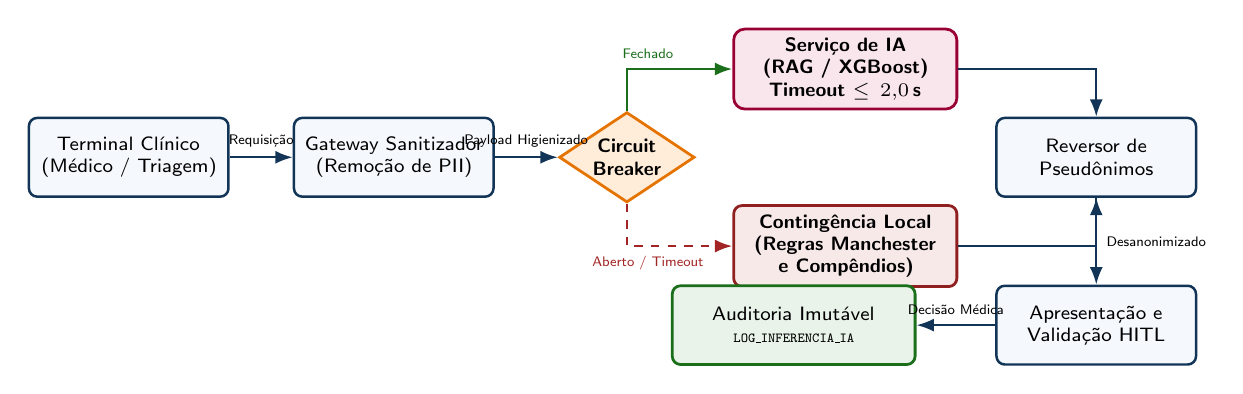
\begin{tikzpicture}[
        box/.style={rectangle, rounded corners=3pt, draw=vitalisdark, fill=vitalislight!40, align=center, minimum height=1.0cm, text width=2.3cm, font=\scriptsize\sffamily, line width=0.9pt},
        aicloud/.style={rectangle, rounded corners=4pt, draw=purple!80!black, fill=purple!10, align=center, minimum height=1.0cm, text width=2.6cm, font=\scriptsize\sffamily\bfseries, line width=1pt},
        breaker/.style={diamond, aspect=1.5, draw=orange!90!black, fill=orange!15, align=center, font=\scriptsize\sffamily\bfseries, line width=1pt, inner sep=1pt},
        fallback/.style={rectangle, rounded corners=3pt, draw=vitalisred!80!black, fill=vitalisred!10, align=center, minimum height=1.0cm, text width=2.6cm, font=\scriptsize\sffamily\bfseries, line width=1pt},
        audit/.style={rectangle, rounded corners=3pt, draw=vitalisgreen!80!black, fill=vitalisgreen!10, align=center, minimum height=1.0cm, text width=2.85cm, font=\scriptsize\sffamily, line width=1pt},
        arrow/.style={-{Latex[length=2.2mm]}, draw=vitalisdark, line width=0.8pt},
        redarrow/.style={-{Latex[length=2.2mm]}, draw=vitalisred!90!black, line width=0.9pt, dashed},
        greenarrow/.style={-{Latex[length=2.2mm]}, draw=vitalisgreen!80!black, line width=0.9pt}
    ]

        % Linha superior: Ingestão e Decisão
        \node (ui) [box] {Terminal Clínico\\(Médico / Triagem)};
        \node (gateway) [box, right=0.8cm of ui] {Gateway Sanitizador\\(Remoção de PII)};
        \node (circuit) [breaker, right=0.8cm of gateway] {Circuit\\Breaker};

        % Bifurcação: IA Externa vs Motor Determinístico
        \node (llm) [aicloud, above right=0.3cm and 0.9cm of circuit] {Serviço de IA\\(RAG / XGBoost)\\Timeout $\le 2{,}0\,\text{s}$};
        \node (determ) [fallback, below right=0.3cm and 0.9cm of circuit] {Contingência Local\\(Regras Manchester\\e Compêndios)};

        % Linha inferior / Saída
        \node (revert) [box, right=3.8cm of circuit] {Reversor de\\Pseudônimos};
        \node (resp) [box, below=1.1cm of revert] {Apresentação e\\Validação HITL};
        \node (log) [audit, left=1.0cm of resp] {Auditoria Imutável\\{\tiny\texttt{LOG\_INFERENCIA\_IA}}};

        % Conexões
        \draw [arrow] (ui) -- node[above, font=\tiny\sffamily] {Requisição} (gateway);
        \draw [arrow] (gateway) -- node[above, font=\tiny\sffamily] {Payload Higienizado} (circuit);
        
        \draw [greenarrow] (circuit.north) |- node[pos=0.6, above, font=\tiny\sffamily, color=vitalisgreen!80!black] {Fechado} (llm.west);
        \draw [redarrow] (circuit.south) |- node[pos=0.6, below, font=\tiny\sffamily, color=vitalisred!90!black] {Aberto / Timeout} (determ.west);
        
        \draw [arrow] (llm.east) -| (revert.north);
        \draw [arrow] (determ.east) -| (revert.south);
        \draw [arrow] (revert) -- node[right, font=\tiny\sffamily] {Desanonimizado} (resp);
        \draw [arrow] (resp) -- node[above, font=\tiny\sffamily] {Decisão Médica} (log);

    \end{tikzpicture}
    \caption{Fluxo de inferência clínica com higienização de dados, resiliência por Circuit Breaker e contingência determinística.}
    \label{fig:fluxo_ia_resiliencia}
\end{figure}

% ==============================================================================
\subsection{Auditoria e Explicabilidade: Tabela \texttt{LOG\_INFERENCIA\_IA}}
\label{subsec:ia_auditoria}

A rastreabilidade integral das operações de inteligência artificial é garantida pela persistência relacional imutável de cada ciclo de inferência na tabela \texttt{LOG\_INFERENCIA\_IA} (requisito \textbf{RF-019}). Essa estrutura fornece respaldo médico-legal, viabiliza auditorias de conformidade com a LGPD e permite a avaliação contínua de degradação (\textit{model drift}) ou viés algorítmico.

\subsubsection{Modelo de Dados Relacional e Trilha Imutável}
Cada registro gerado reflete uma interação individual de suporte clínico, armazenando métricas de desempenho técnico, a resposta textual/estruturada gerada e a deliberação soberana do profissional de saúde. A Listagem~\ref{lst:ddl_log_inferencia} apresenta o esquema DDL em PostgreSQL com restrições de integridade e regras de imutabilidade.

\begin{lstlisting}[language=SQL, caption={Definição DDL da tabela imutável \texttt{LOG\_INFERENCIA\_IA}}, label={lst:ddl_log_inferencia}]
-- Tabela imutavel para auditoria de inferencias clinicas de IA
CREATE TABLE log_inferencia_ia (
    id UUID PRIMARY KEY DEFAULT gen_random_uuid(),
    atendimento_id UUID NOT NULL,
    usuario_id UUID NOT NULL,
    modulo_ia VARCHAR(40) NOT NULL, -- 'COPILOTO_PRESCRICAO', 'SEPSE_PREDICAO'
    modelo_ia_versao VARCHAR(60) NOT NULL, -- ex: 'vitalis-rag-med-v2.1', 'xgb-sepsis-v1.4'
    prompt_sanitizado_hash CHAR(64) NOT NULL, -- Hash SHA-256 do payload enviado
    tokens_prompt INTEGER NOT NULL DEFAULT 0,
    tokens_resposta INTEGER NOT NULL DEFAULT 0,
    latencia_ms INTEGER NOT NULL, -- Tempo de resposta em milissegundos
    score_confianca NUMERIC(4,3) CHECK (score_confianca >= 0.0 AND score_confianca <= 1.0),
    modo_contingencia_ativo BOOLEAN NOT NULL DEFAULT FALSE,
    resposta_ia JSONB NOT NULL,
    decisao_medica VARCHAR(20) NOT NULL, -- 'ACEITA', 'MODIFICADA', 'REJEITADA'
    justificativa_humana TEXT, -- Obrigatorio para decisoes 'MODIFICADA' ou 'REJEITADA'
    criado_em TIMESTAMP WITH TIME ZONE NOT NULL DEFAULT CURRENT_TIMESTAMP,
    decidido_em TIMESTAMP WITH TIME ZONE,
    
    CONSTRAINT fk_log_atendimento FOREIGN KEY (atendimento_id) REFERENCES atendimento(id),
    CONSTRAINT fk_log_usuario FOREIGN KEY (usuario_id) REFERENCES usuario(id),
    CONSTRAINT chk_justificativa_obrigatoria CHECK (
        (decisao_medica IN ('MODIFICADA', 'REJEITADA') AND justificativa_humana IS NOT NULL AND LENGTH(TRIM(justificativa_humana)) >= 10)
        OR (decisao_medica = 'ACEITA')
    )
);

-- Indices otimizados para investigacao clinica e relatorios de governanca
CREATE INDEX idx_log_ia_atendimento ON log_inferencia_ia (atendimento_id);
CREATE INDEX idx_log_ia_modulo_criacao ON log_inferencia_ia (modulo_ia, criado_em);
CREATE INDEX idx_log_ia_decisao ON log_inferencia_ia (decisao_medica);

-- Gatilho de seguranca para impedir remocao ou alteracao (imutabilidade estrita)
CREATE OR REPLACE FUNCTION trg_impedir_mutacao_log_ia()
RETURNS TRIGGER AS $$
BEGIN
    RAISE EXCEPTION 'Operacao negada: registros de LOG_INFERENCIA_IA sao estritamente imutaveis (WORM).';
END;
$$ LANGUAGE plpgsql;

CREATE TRIGGER trg_bloqueio_modificacao_log_ia
BEFORE UPDATE OR DELETE ON log_inferencia_ia
FOR EACH ROW EXECUTE FUNCTION trg_impedir_mutacao_log_ia();
\end{lstlisting}

\subsubsection{Governança de IA e Monitoramento Pós-Implantação}
A estrutura de dados da tabela \texttt{LOG\_INFERENCIA\_IA} viabiliza a geração de painéis analíticos contínuos para o Comitê de Ética Médica e a Governança de TI do hospital:
\begin{itemize}
    \item \textbf{Taxa de Aderência Clínica (\textit{Acceptance Rate})}: Razão entre decisões aceitas e o total de inferências emitidas por especialidade e por modelo, permitindo identificar precocemente módulos com alta taxa de rejeição;
    \item \textbf{Análise de Justificativas de Rejeição}: Agrupamento semântico das motivações clínicas apresentadas por médicos ao descartar alertas, identificando hipóteses em que os protocolos institucionais divergem das bulas da ANVISA ou demandam recalibração do re-ranqueador;
    \item \textbf{Detecção de Desvio Conceitual (\textit{Model Drift})}: Monitoramento contínuo da distribuição estatística de latência, pontuações de confiança e frequência de acionamento do Circuit Breaker, sinalizando a necessidade de re-treinamento dos comitês de árvores do motor de sepse.
\end{itemize}

Dessa forma, o Vitalis v2.0 articula conformidade regulatória, integridade científica e segurança operacional no aproveitamento dos recursos de inteligência artificial em saúde humana.

\newpage

% ==============================================================================
% REFERÊNCIAS BIBLIOGRÁFICAS
% ==============================================================================
\bibliographystyle{plain}
\bibliography{referencias}

\end{document}
